\documentclass[11pt,a4paper]{article}
\usepackage[T1]{fontenc}
\usepackage[utf8]{inputenc}
\usepackage{lmodern}
\usepackage[margin=2.4cm]{geometry}
\usepackage{booktabs}
\usepackage{array}
\usepackage{tabularx}
\usepackage{longtable}
\usepackage{xcolor}
\usepackage{amsmath,amssymb}
\usepackage{pgfplots}
\usepackage{pgfplotstable}
\usepackage{caption}
\usepackage{enumitem}
\usepackage{listings}
\usepackage[colorlinks=true,linkcolor=blue!50!black,urlcolor=blue!50!black]{hyperref}
\pgfplotsset{compat=1.17}
\usepgfplotslibrary{groupplots}
\usetikzlibrary{positioning,arrows.meta,shapes.misc,fit,calc}
\captionsetup{font=small,labelfont=bf}
\setlist{nosep,leftmargin=1.4em}
\setlength{\parindent}{0pt}
\setlength{\emergencystretch}{3em}
\renewcommand{\_}{\textunderscore\hspace{0pt}}
\setlength{\parskip}{0.45em}
\renewcommand{\arraystretch}{1.08}
\usepackage[compact]{titlesec}
\titlespacing*{\section}{0pt}{1.4em}{0.5em}
\titlespacing*{\subsection}{0pt}{1.0em}{0.35em}
\setcounter{tocdepth}{2}
\renewcommand{\floatpagefraction}{0.8}
\renewcommand{\topfraction}{0.9}
\renewcommand{\textfraction}{0.1}

\lstset{basicstyle=\ttfamily\small,columns=fullflexible,breaklines=true,frame=single,framerule=0.3pt,rulecolor=\color{gray!60},xleftmargin=0.5em,xrightmargin=0.5em}

% open items are shown in red
\newcommand{\todo}[1]{\textcolor{red}{\textbf{[TODO: #1]}}}
\newcommand{\file}[1]{\texttt{\small #1}}
\newcommand{\env}[1]{\texttt{#1}}
\newcommand{\code}[1]{\texttt{#1}}
\newcommand{\sweep}{s\,/\,sweep}
\newcommand{\dis}[1]{\par\smallskip\noindent\fbox{\parbox{\dimexpr\linewidth-2\fboxsep-2\fboxrule}{\small\textbf{Code and documents disagree.} #1}}\par\smallskip}
\newcommand{\Ndim}{N}
\newcommand{\Lt}{L_{\rm trot}}
\newcommand{\NFL}{N_{\rm FL}}
\newcommand{\Nd}{N_{\rm d}}
\newcommand{\Op}{\mathrm{Op}}
\newcommand{\dt}{\Delta\tau}

% plot styles (colour-blind safe, also distinguishable by marker); same as the short report
\definecolor{cA30}{HTML}{1B9E77}
\definecolor{cH100}{HTML}{D95F02}
\definecolor{cMAX}{HTML}{7570B3}
\definecolor{cMI}{HTML}{E7298A}
\definecolor{cCPU}{HTML}{666666}
\pgfplotsset{
  every axis/.append style={
    grid=major, grid style={gray!25}, tick label style={font=\small},
    label style={font=\small}, legend style={font=\scriptsize, fill=white, fill opacity=0.85, text opacity=1, draw=gray!50},
    unbounded coords=jump,
  },
  a30/.style={color=cA30, mark=square*, thick},
  h100/.style={color=cH100, mark=triangle*, thick},
  max/.style={color=cMAX, mark=diamond*, thick},
  mi/.style={color=cMI, mark=*, thick},
  cpu/.style={color=cCPU, mark=x, thick},
  mybars/.style={ybar, bar width=9pt},
}
\tikzset{
  box/.style={draw, rounded corners=2pt, align=center, font=\small, inner sep=4pt},
  hostbox/.style={box, fill=gray!12},
  devbox/.style={box, fill=cA30!15},
  arr/.style={-{Stealth[length=2mm]}, thick},
}

\title{How ALF was ported to GPUs\\[0.3em]
\large The implementation of the auxiliary-field QMC sweep on NVIDIA, Intel and AMD accelerators\\[0.2em]
\normalsize Branch \texttt{gpu-port-unified}, state of 2026-11-13}
\author{[author]}
\date{2026-11-13}

\begin{document}
\maketitle
\tableofcontents
\newpage

\section{Reader's guide and summary}
\label{sec:guide}

\subsection{What this document is}

This document describes how the finite-temperature sweep of ALF was moved onto graphics processors (GPUs). It is written for a reader who knows the auxiliary-field QMC algorithm and the CPU code of ALF well, but who has not programmed a GPU. It complements the shorter report \file{docs/gpu/report/gpu\_port\_report.tex}, which summarises status, speed and open items. That report is not repeated here. This document explains the implementation: which data live where, which mathematics each device routine evaluates, why the code is organised the way it is, and what each design choice cost or gained.

The ground truth is the source code of the branch \texttt{gpu-port-unified} as of 2026-11-13. File and line references are given as \file{file:line}. The Markdown notes in \file{docs/gpu/} are used for history, measurements and decisions. Every number taken from a note carries a \LaTeX{} comment with the source file next to it. Where the code and a note disagree, the text follows the code and a framed box records the disagreement. Items that could not be determined are marked \todo{like this}.

\subsection{How to read it}

\begin{itemize}
\item Section~\ref{sec:cpu} restates the CPU sweep in the notation of the ALF documentation and gives the measured CPU cost of each part. It says which operations had to move and why.
\item Section~\ref{sec:design} gives the design decisions: the programming model, the library layer \texttt{alf\_la} with a table of every routine and its implementation per vendor, and the principle of a device-resident Green function.
\item Section~\ref{sec:data} lists every device array, its size as a function of $N$, $\Lt$, $\NFL$ and \texttt{Nwrap}, and every transfer between host and device in one sweep.
\item Sections~\ref{sec:wrap} to~\ref{sec:obs} are the core: propagation, stabilisation, local updates and measurements on the device, each with the formulas as coded.
\item Section~\ref{sec:mpi} covers MPI, parameter-parallel runs and sharing a GPU between ranks.
\item Section~\ref{sec:backends} describes the three vendor backends, the problems met and their solutions.
\item Sections~\ref{sec:verif} and~\ref{sec:perf} give verification and performance.
\item Sections~\ref{sec:notported} and~\ref{sec:lessons} say what is not ported, what it would take, and what we learned for a port of the whole of ALF.
\item The appendix has a glossary of GPU terms (Appendix~\ref{app:glossary}); readers new to GPUs may want to read it first. It also has a file-by-file guide to the GPU source and the build lines.
\end{itemize}

\subsection{Summary of the implementation}

\paragraph{What runs where.} In a GPU build the following parts of the sweep run on the accelerator (the \emph{device}); the CPU is called the \emph{host}.
\begin{itemize}
\item The Green function $G$ of every flavour lives on the device for the whole sweep. The host copy is updated only when host code needs it (ticket 208-1, \file{gpu\_update\_mod.F90:52-53}).
\item Propagation $G\to B G B^{-1}$ by the hopping and the interaction vertices: own kernels for checkerboard groups and vertices, vendor matrix products for dense hopping.
\item Stabilisation: the $UDV$ stacks, the QR decompositions, the assembly of $G$ from the left and right decompositions (\texttt{CGR}), the precision check and the phase of the determinant.
\item Local updates: the gathers of matrix elements and the flushes of the delayed and submatrix schemes. The proposal, the ratio arithmetic on small matrices, the Metropolis decision and the random numbers stay on the host, so that the GPU run follows the same Markov chain as the CPU run with the same seed.
\item Equal-time observables of the Hubbard model (including the point-defect observables) and the time-displaced pass with its observables.
\end{itemize}

\paragraph{How.} Own kernels are written as OpenMP \texttt{target} regions in the existing Fortran files. All dense linear algebra goes through one new module, \texttt{alf\_la}, whose routines call cuBLAS/cuSOLVER (NVIDIA), oneMKL (Intel) or hipBLAS/hipSOLVER and own HIP kernels (AMD), or plain BLAS/LAPACK in a CPU build. The backend is selected by \texttt{configure.sh GPU=none|nvidia|intel|amd}. A build with \texttt{GPU=none} is bitwise identical to upstream ALF (with \texttt{LOBS\_ST=1}; \file{CONSOLIDATION.md}). The GPU code is in seven new modules \file{Prog/gpu\_*.F90} (about 12\,500 lines) plus the library layer (about 5\,900 lines of Fortran, C++, SYCL and HIP). The CPU code is touched only by guarded early branches.

\paragraph{The four ideas that made it fast.}
\begin{enumerate}
\item \textbf{Keep $G$ and the stacks on the device.} Moving an $N\times N$ complex matrix across PCIe costs more than most operations on it. Only scalars, short vectors and small blocks cross the bus during a sweep (Section~\ref{sec:data}).
\item \textbf{Replace the rank-one update by the submatrix update in block mode.} One sequential rank-one update per site is bound by the latency of the device (about 10 to 30~$\mu$s per operation), not by its arithmetic. The block mode moves all per-site work to a small host matrix and leaves the device two matrix products per block (Section~\ref{sec:updates}). On the A30 this is 2.4 to 5 times faster than the standard update.
\item \textbf{Replace pivoted QR by pre-pivoted QR.} No GPU library has a fast QR with column pivoting. Sorting the columns by their norms once and then doing an unpivoted QR gives the same precision for the default stabilisation (Section~\ref{sec:stab}).
\item \textbf{Write own kernels where the vendor library is weak.} oneMKL's QR runs its panels on the host, rocSOLVER's QR launches thousands of tiny kernels, and the OpenMP runtime of GCC for AMD costs 150~$\mu$s per launch. Own QR kernels in SYCL and HIP, HIP kernels for the small operations, an asynchronous SYCL path for the update blocks, and a patched GCC plugin removed these bottlenecks (Section~\ref{sec:backends}).
\end{enumerate}

\paragraph{Results.} For the production model (Hubbard model with a space-time point defect, $\beta=L$, $\dt=0.1$, $N=L^2$) one sweep at $L=24$ takes 3.5 to 5.3~s on one GPU (H100 3.51, Max~1550 tile 4.04 to 4.96, MI210 4.41, A30 5.25). % helma_h100.md 4.1; SPEEDUPS.md; amd_mi210/README.md; TUNING_DEFECT.md
On one CPU thread the same build takes 148.6~s (A30 host, \file{TUNING\_DEFECT.md}). % TUNING_DEFECT.md
One chain does not fill a GPU; with several chains per GPU (MPS on NVIDIA, CCS on Intel) the throughput per GPU rises by a factor 2 to 4 (Section~\ref{sec:mpi}). The GPU runs reproduce the CPU runs of the same compiler and seed to $10^{-13}$ to $10^{-15}$ in the observables for \texttt{Mz=.F.} (Section~\ref{sec:verif}).

\paragraph{Limits.} The port covers one model family: Hubbard-type models with diagonal single-site vertices and discrete fields, finite temperature, sequential local updates. Everything else is refused at setup and runs on the CPU (Section~\ref{sec:notported}).

\subsection{How the port came about}

The chronology matters for reading the code, because several comments still describe intermediate states.
\begin{itemize}
\item \textbf{Phase 0 and 1} (to 2026-10-27): CPU profile and baseline, kernel micro-benchmarks on the A30, prototypes of OpenMP and OpenACC launch costs; ADR-001 (programming model) and ADR-002 (\texttt{alf\_la} and data model) accepted at the Phase~1 gate on 2026-10-27 (\file{PLAN.md}, section 5).
\item \textbf{Phase 2, tickets 201 to 208} (2026-10-27 to 2026-11-03): the NVIDIA minimum viable product. 201--206: \texttt{alf\_la}, the mirror, wraps, rank-one update, stabilisation; 207: the $\tau$ pass; 208-1: $G$ device-authoritative; 208-2 and 208-3: equal-time and $\tau$ observables on the device. Ticket 212 made all reductions deterministic. This phase was slowed by the verification process described in Section~\ref{sec:verif}, until the owner's decision 41 of 2026-11-02.
\item \textbf{After 2026-11-02} (about seven days, \file{EVAL\_ORIGINAL\_GPU\_BRANCH.md}): CPU delayed and submatrix updates taken into the branch and ported to the device with block mode; time-dependent hopping for the point defect; MPI and parameter-parallel runs; H100 on Helma; Max~1550 production on SuperMUC-NG Phase~2 with the staging buffer, the asynchronous block path and the own SYCL QR; the AMD backend with HIP kernels and own HIP QR.
\item \textbf{2026-11-13}: the vendor lines were merged with \texttt{--no-ff} into \texttt{gpu-port-unified} (\file{CONSOLIDATION.md}): first the parameter-parallel and optimisation lines of the NVIDIA work, then the Intel production and team lines, then AMD. Conflicts were in \file{alf\_la\_mod.F90}, \file{gpu\_lowrank\_mod.F90}, \file{gpu\_obs\_mod.F90}, \file{configure.sh} and job files. In \file{gpu\_lowrank\_mod.F90} the Intel kernels are the base and the HIP calls are applied under \texttt{ALF\_LA\_HIP}; in \file{gpu\_obs\_mod.F90} the summation order of NVIDIA and Intel was kept and AMD uses its HIP kernels. The LU-free phase was added the same day.
\end{itemize}


\subsection{Notation}

\begin{tabular}{@{}lp{11.5cm}@{}}
$N$ & number of orbitals, \texttt{Ndim}; $N=L^2$ for the square lattice of side $L$\\
$\Lt$ & number of time slices, $\beta/\dt$\\
$\NFL$ & number of flavours; $N_{\rm FL,eff}$ the number actually computed (\texttt{Calc\_Fl})\\
$\Nd$ & \texttt{N\_delay}, the maximal rank of a pending low-rank correction\\
$N_{\rm ST}$ & number of stabilisation points, \texttt{NSTM}, about $\Lt/\texttt{Nwrap}$\\
$B_\tau$ & propagator of slice $\tau$, $B_\tau = e^{-\dt K}\,\prod_n e^{V_n(\sigma_{n,\tau})}$ (order as in ALF)\\
$B(\tau_2,\tau_1)$ & $B_{\tau_2}\cdots B_{\tau_1+1}$\\
$G(\tau)$ & equal-time Green function $\langle c_i c_j^\dagger\rangle$ at slice $\tau$, $[1+B(\tau,0)B(\beta,\tau)]^{-1}$\\
D$\to$H, H$\to$D & copy from device to host, from host to device\\
\end{tabular}

\section{The sweep as ALF does it on the CPU}
\label{sec:cpu}

This section restates the finite-temperature sweep of \file{Prog/main.F90} in the notation of the ALF documentation. Its purpose is to name every operation that the GPU code replaces, with its cost, so that the later sections can refer to it.

\subsection{Propagators and the Green function}

For a given configuration of the auxiliary fields $\sigma_{n,\tau}$ the fermion weight is $\prod_{f}\det[1+B_f(\beta,0)]^{N_{\rm SUN}}$, with one propagator per flavour $f$,
\begin{equation}
B(\tau_2,\tau_1) = \prod_{\tau=\tau_1+1}^{\tau_2} B_\tau ,\qquad
B_\tau = e^{-\dt T}\prod_{n} e^{\,g_n\,\eta(\sigma_{n,\tau})\,V_n}\,,
\end{equation}
where the order of the factors is that of \texttt{Op\_T} and \texttt{Op\_V} in the Hamiltonian. The hopping exponential $e^{-\dt T}$ is either one dense matrix or a product of \emph{checkerboard} factors, one per element of \texttt{Op\_T}, each acting on a few sites (\texttt{Hop\_mod.F90}). With \texttt{Symm=.T.} the hopping is split symmetrically, $e^{-\dt T/2}\,V\,e^{-\dt T/2}$, and observables are measured on the transformed Green function $e^{\dt T/2}\,G\,e^{-\dt T/2}$ (\texttt{Hop\_mod\_Symm}).

For the Hubbard model each vertex $\Op_V(n)$ acts on one site $p_n$ with $N_{\rm non\text{-}zero}=1$, so $e^{V_n}$ is the identity except for one diagonal element $e^{\alpha\,\sigma}$. The equal-time Green function at slice $\tau$ is
\begin{equation}
G(\tau) = \left[1 + B(\tau,0)\,B(\beta,\tau)\right]^{-1}.
\end{equation}

\subsection{Wrapping}

Between stabilisations, $G$ is moved from slice $\tau$ to $\tau+1$ by a similarity transformation,
\begin{equation}
G(\tau+1) = B_{\tau+1}\,G(\tau)\,B_{\tau+1}^{-1},
\end{equation}
and in the downward direction by the inverse. In ALF this is \texttt{WRAPGRUP} and \texttt{WRAPGRDO} (\file{Wrapgr\_mod.F90}). They are interleaved with the local updates: on the way up, the hopping is applied (\texttt{Hop\_mod\_mmthr}, \texttt{Hop\_mod\_mmthl\_m1}), then for every vertex $n$ in order the vertex factor of the old field is wrapped in (\texttt{Op\_Wrapup}) and the field on that vertex is updated. On the way down the order is reversed. The wrap of one vertex is a scaling of row $p$ by $z_a$ and column $p$ by $z_b=1/z_a$:
\begin{equation}
G_{rj}\to z_a G_{rj},\quad G_{jr}\to z_b G_{jr}\qquad (r=p_n).
\end{equation}
The hopping part costs two $N^3$ products per slice with dense hopping, or $O(N^2)$ with checkerboard factors.

\subsection{Stabilisation with $UDV$ stacks}

Products of many $B_\tau$ are ill conditioned: their singular values span many orders of magnitude. ALF therefore keeps the products in factorised form,
\begin{equation}
B(\tau,0) = U_R D_R V_R ,\qquad B(\beta,\tau) = V_L^{\dagger} D_L U_L^{\dagger},
\end{equation}
with $U$ unitary, $D$ diagonal with the scales, and $V$ well conditioned (upper triangular times a permutation). Every \texttt{Nwrap} slices, \texttt{WRAPUR} (or \texttt{WRAPUL}) multiplies the next \texttt{Nwrap} propagators onto $U D$ and re-factorises with a QR decomposition with column pivoting (\texttt{UDV\_mod}, \texttt{QDRP\_decompose}, LAPACK \texttt{ZGEQP3}):
\begin{equation}
B(\tau_2,\tau_1)\,U D = Q R P^{T},\qquad U\leftarrow Q,\; D\leftarrow |{\rm diag}\,R|,\; V\leftarrow D^{-1}R P^{T} V .
\end{equation}
The decompositions at the stabilisation points are kept in a stack \texttt{udvst}($N_{\rm ST}$ slots per flavour). On the upward pass the right decompositions are built and the left ones read from the stack; on the downward pass the reverse. With \texttt{STABLOG} the scales are kept as logarithms.

At each stabilisation point $G$ is computed afresh from the two decompositions (\texttt{CGR}, \file{cgr1\_mod.F90}):
\begin{equation}
\label{eq:cgr}
G = \left[1 + U_R D_R V_R V_L D_L U_L^\dagger\right]^{-1}
  = U_L\left[\,U_R^\dagger U_L + D_R V_R V_L D_L\,\right]^{-1} U_R^\dagger .
\end{equation}
The bracket is formed with the scales applied on the outside and is again inverted by a pivoted QR. The phase of $\det G$ is tracked from the same factors. \texttt{Control\_PrecisionG} compares the fresh $G$ with the wrapped one and stops the run when the difference exceeds a threshold.

\subsection{Local updates}

For a proposed change of the field on vertex $n$ at slice $\tau$, with $\Delta = e^{\,g\,(\eta_{\rm new}-\eta_{\rm old})\,V}-1$ on site $p$, the ratio of weights is
\begin{equation}
R = \prod_f\left[1+\Delta_f\,(1-G_{pp})\right]^{N_{\rm SUN}}\,\frac{\gamma_{\rm new}}{\gamma_{\rm old}}\,e^{\ldots},
\end{equation}
and on acceptance (\texttt{Upgrade2}, Sherman--Morrison)
\begin{equation}
\label{eq:rank1}
G' = G - \frac{\Delta}{1+\Delta(1-G_{pp})}\;G_{:,p}\,\bigl(e_p^T - G_{p,:}\bigr).
\end{equation}
This is one \texttt{ZGERU} of size $N\times N$, $8N^2$ flops and $32N^2$ bytes of memory traffic per accepted flip, and there are $2\,N\,\Lt$ proposals per sweep (each vertex on the way up and on the way down). The branch also contains CPU versions of the \emph{delayed} and \emph{submatrix} schemes (\file{Lowrank\_update\_mod.F90}, parameter \texttt{Sequential\_scheme}; ported on 2026-11-06 from the fork branch \texttt{feature/delayed-submatrix-clean}, commit \texttt{80c1c80d}, and listed in \file{GPU\_PLAN\_V2.md} as a prerequisite of an upstream merge), which collect up to $\Nd$ accepted flips and apply them as one matrix product (Section~\ref{sec:updates}).

\subsection{Measurements}

Equal-time observables are measured on every slice from $G(\tau)$ by the Hamiltonian's \texttt{Obser} routine. For the Hubbard model these are the kinetic, potential and total energy, the density, and the equal-time correlation functions (Green, spin, density) accumulated as functions of the distance $i-j$ on the lattice. With \texttt{Ltau=1}, a second pass after the sweep computes $G(\tau,0)$, $G(0,\tau)$ and $G(\tau,\tau)$ for all $\tau$ and calls \texttt{ObserT}. That pass has its own stabilisation, \texttt{CGR2\_2}, which inverts a $2N\times 2N$ block matrix with a pivoted QR.

\subsection{Measured CPU cost per part}

Table~\ref{tab:cpuprof} shows where one CPU core spends its time. The numbers are from stack sampling of upstream ALF (GNU 13.3, OpenBLAS, one rank, one thread) for the plain Hubbard model ($U=4$, $\beta=4$, $\dt=0.1$, \texttt{Nwrap}=10, \texttt{Ltau=1}) on three lattices with checkerboard (cb) and dense hopping (\file{PROFILE.md}). They are for the reference model of the profile, not for the point-defect model.

\begin{table}[h]
\centering
\caption{Share of wall time in percent per routine on one CPU core (\file{PROFILE.md}, section ``Result''). $N=144, 400, 1024$.}
\label{tab:cpuprof}
\small
\begin{tabular}{@{}lrrrrrr@{}}
\toprule
 & \multicolumn{3}{c}{checkerboard} & \multicolumn{3}{c}{dense} \\
\cmidrule(lr){2-4}\cmidrule(lr){5-7}
Routine & $12^2$ & $20^2$ & $32^2$ & $12^2$ & $20^2$ & $32^2$ \\
\midrule
\texttt{CGR2\_2} ($\tau$ pass, $2N\times2N$) & 27.7 & 29.4 & 23.6 & 19.1 & 16.5 & 14.4 \\ % PROFILE.md
\texttt{CGR} & 12.7 & 15.0 & 11.2 & 7.4 & 8.8 & 7.1 \\ % PROFILE.md
UDV decompose & 6.6 & 11.0 & 7.5 & 5.5 & 6.7 & 4.9 \\ % PROFILE.md
\texttt{Upgrade2} rank-1 (\texttt{ZGERU}) & 17.2 & 23.5 & 33.3 & 9.7 & 15.2 & 20.1 \\ % PROFILE.md
\texttt{Upgrade2} ratio & 3.2 & 1.0 & 0.4 & 1.7 & 0.6 & 0.3 \\ % PROFILE.md
\texttt{Op\_Wrapup/do} & 2.1 & 0.8 & 1.2 & 1.4 & 0.4 & 0.6 \\ % PROFILE.md
\texttt{WRAPUR/UL} $B$ products & 4.5 & 2.0 & 5.8 & 14.7 & 12.0 & 13.4 \\ % PROFILE.md
\texttt{PROPR/PROPRM1} & 4.6 & 2.0 & 4.7 & 12.4 & 13.6 & 14.3 \\ % PROFILE.md
Hopping in \texttt{WRAPGR} & 3.0 & 1.6 & 2.8 & 14.5 & 16.8 & 14.3 \\ % PROFILE.md
\texttt{ObserT} & 5.0 & 3.9 & 1.9 & 4.3 & 2.2 & 1.2 \\ % PROFILE.md
\texttt{Obser} & 11.9 & 7.6 & 6.2 & 7.4 & 4.1 & 3.9 \\ % PROFILE.md
\midrule
Stabilisation (sum) & 47.0 & 55.4 & 42.3 & 32.0 & 32.0 & 26.4 \\ % PROFILE.md aggregates
Local updates (sum) & 22.5 & 25.3 & 34.9 & 12.8 & 16.2 & 21.0 \\ % PROFILE.md
$B$ products (sum) & 12.1 & 5.6 & 13.3 & 41.6 & 42.4 & 42.0 \\ % PROFILE.md
Measurements (sum) & 16.9 & 11.5 & 8.1 & 11.7 & 6.3 & 5.1 \\ % PROFILE.md
Whole $\tau$ pass & 41.3 & 40.2 & 34.3 & 40.8 & 36.5 & 35.3 \\ % PROFILE.md
\midrule
Wall time per sweep (s) & 0.60 & 8.0 & 193 & 0.80 & 13.7 & 294 \\ % PROFILE.md
\bottomrule
\end{tabular}
\end{table}

The call counts per sweep at $12^2$ with checkerboard are: \texttt{upgrade2} 11\,520, \texttt{op\_wrap} 46\,080, \texttt{cgr} 16, \texttt{cgr2\_2} 8, \texttt{decompose} 24, \texttt{obser} 79, \texttt{obsert} 41 (\file{PROFILE.md}). % PROFILE.md
By kind of leaf routine, 23\,\% of the time is BLAS-3, 35\,\% BLAS-1/2 and 31\,\% plain Fortran loops of ALF (\file{PROFILE.md}, $12^2$ cb). % PROFILE.md

\subsection{The production model}

The port was driven by one model: the Hubbard model on the square lattice with $\pi$ flux and a space-time point defect (\file{point\_defect\_math.tex}; the predefined \texttt{Hamiltonian\_Hubbard} with \texttt{ham\_h0}$\ne0$):
\begin{equation}
H = -t\sum_{\langle ij\rangle\sigma}\bigl(e^{iA_{ij}}c^\dagger_{i\sigma}c_{j\sigma}+{\rm h.c.}\bigr) + U\sum_i\bigl(n_{i\uparrow}-\tfrac12\bigr)\bigl(n_{i\downarrow}-\tfrac12\bigr),
\end{equation}
with $N=L^2$ sites and discrete Ising auxiliary fields; the production parameter file has $\NFL=2$ and $N_{\rm SUN}=2$ (\file{TUNING\_DEFECT.md}), and the pinning field requires $\NFL=2$. The defect is a pinning field on one site at one time slice. In the code (\file{Hamiltonian\_Hubbard\_smod.F90:495-525}) it is a second hopping element per flavour, \texttt{Op\_T(2,nf)}, diagonal with $\mp h_0$ on the pin site $N/2-L/2$, with a time-dependent coupling $g_t(\tau)$ that is $-1$ on the first slice and 0 elsewhere. So the propagator of slice 1 carries the extra factor $e^{\pm h_0 n_{p\sigma}}$, a pulse of strength $h_0$ in $S^z_p$ at $\tau=0$. The static hopping \texttt{Op\_T(1,nf)} is a dense $N\times N$ matrix; the \texttt{Checkerboard} flag is ignored when the pin is on. The production parameters are \texttt{Mz=.F.}, $U=5$ (and a scan 5.15 to 5.425), $h_0=1$, \texttt{Symm=.T.}, $\dt=0.1$, $\beta=L$ (so $\Lt=10L$), \texttt{Ltau=0}, \texttt{Nwrap}=10 (\file{TUNING\_DEFECT.md}; \file{DECISIONS.md}, item 47). The new observables are \texttt{SpinZ\_local} and \texttt{SpinZ\_localtau}, the response $\langle S^z_j(\tau)\rangle$ to the pulse.

For the GPU the model has three consequences: the hopping is dense, so the wraps are matrix products (good for a GPU); the defect is a time-dependent hopping element, which needed its own device path (Section~\ref{sec:wrap}); and the vertices are single-site and diagonal, which makes the submatrix update in block mode possible (Section~\ref{sec:updates}).

\dis{\file{point\_defect\_math.tex} places the pulse on the two slices $\Lt/2$ and $\Lt/2+1$ with $g_t=-\tfrac12$ each, and recommends the projector code and \texttt{Mz=.T.}. The code puts the pulse on slice 1 with $g_t=-1$ (after the merge of 2026-11-09), \texttt{Ham\_Set} refuses the pin with the projector, and production uses finite temperature with \texttt{Mz=.F.}.}


\subsection{What this means for a GPU}

A GPU is fast for large dense matrix products and for simple loops over many independent elements, and slow for anything sequential or small (Appendix~\ref{app:glossary}). Read with that in mind, the profile says:

\begin{itemize}
\item \textbf{Stabilisation} is the largest group (26 to 55\,\%). It consists of QR factorisations, triangular solves and matrix products of size $N$ or $2N$. These map well to vendor libraries, except that \emph{pivoted} QR (\texttt{ZGEQP3}) does not exist on GPUs (Section~\ref{sec:stab}).
\item \textbf{Local updates} grow with $N$ (17 to 33\,\% for the rank-one update alone). A rank-one update is memory bound and strictly sequential: each proposal needs $G_{pp}$ after the previous acceptance. On a GPU each step costs at least one kernel launch and one transfer of $G_{pp}$ to the host, 10 to 30~$\mu$s, while a CPU core does the whole update at $N=144$ in about 7~$\mu$s (\file{BENCHMARKS.md}, Phase 1: rank-1 update 4.7~$\mu$s device and 6.8~$\mu$s host at $N=144$). % BENCHMARKS.md
This is the hardest part of the port (Section~\ref{sec:updates}).
\item \textbf{$B$ products} (wraps) are 6 to 42\,\%: large with dense hopping, small with checkerboard. Dense hopping is a matrix product and maps to the library. Checkerboard needs own kernels (Section~\ref{sec:wrap}).
\item \textbf{Measurements} are 5 to 17\,\%. They read $G$ on every slice. If they stayed on the host, $G$ would have to cross the bus $2\Lt$ times per sweep, which at $N=576$ is about 5~MB per copy and flavour. They had to move too (Section~\ref{sec:obs}).
\end{itemize}

So no single part dominates: a port that moves only the matrix products to the GPU gains little, and every part had to move. That is why the port keeps all large data on the device (Section~\ref{sec:data}).

For the production model the hopping is a dense matrix (the \texttt{Checkerboard} flag is ignored when the pinning field is on, \file{TUNING\_DEFECT.md}), so the CPU sweep is dominated by $N^3$ matrix products. One CPU thread needs 1.68, 12.7 and 148.6~s per sweep at $L=12$, 16 and 24 with $\beta=L$ (nvfortran, submatrix $\Nd=8$, \file{TUNING\_DEFECT.md}). % TUNING_DEFECT.md
A fit gives $t\propto L^{6.44}$ (\file{report/sections/s6\_performance.tex}): $N^3$ per operation times $\Lt\propto L$. % s6_performance.tex tab:fits

\section{Design decisions and why}
\label{sec:design}

\subsection{Constraints}

The brief of the port fixed four constraints (\file{ADR-001-programming-model.md}, ``Context''; \file{CLAUDE.md}):
\begin{enumerate}
\item One Fortran source tree for NVIDIA and Intel GPUs (AMD was added later). The backend is chosen when the code is configured.
\item A build with \texttt{GPU=none} must behave exactly like upstream ALF and must not become slower.
\item No polymorphism or deep copies of derived types on the device; data stay on the device across the sweep; every host--device transfer is documented.
\item The default and the \texttt{STABLOG} stabilisation are the targets.
\end{enumerate}
The compilers set the second boundary. nvfortran (NVIDIA HPC SDK) supports OpenMP offload, OpenACC, CUDA Fortran and offload of \texttt{do concurrent}. ifx (Intel) supports OpenMP offload but not OpenACC. gfortran supports OpenMP offload to AMD GPUs (\file{ADR-001}).

\subsection{Programming model: OpenMP target offload plus vendor libraries}

The decision (ADR-001, accepted 2026-10-27 at the Phase~1 gate) has two parts. % ADR-001-programming-model.md
\begin{enumerate}
\item \textbf{Own kernels are OpenMP 5.x \texttt{target} regions}, written in the Fortran modules next to the data they touch. A conservative subset is used that both nvfortran and ifx compile correctly: \texttt{target enter/exit data}, \texttt{target update}, \texttt{target teams distribute parallel do} over explicit-shape arrays, \texttt{use\_device\_addr}, and \texttt{interop} only inside the library layer. Not used on the device: \texttt{declare mapper}, unified shared memory, the \texttt{loop} construct, polymorphism, allocation, type-bound procedures (\file{ADR-001}, ``Decision'', item 1).
\item \textbf{The cubic work goes to vendor libraries} behind one module, \texttt{alf\_la} (ADR-002): cuBLAS and cuSOLVER on NVIDIA, oneMKL on Intel, hipBLAS and hipSOLVER on AMD, plain BLAS and LAPACK in the CPU build.
\end{enumerate}

\paragraph{Why not the alternatives.} The ADR lists them with the reason for rejection (\file{ADR-001}, ``Alternatives considered''):
\begin{itemize}
\item \emph{OpenACC}: NVIDIA only in practice (ifx has none), so a second set of directives would be needed for Intel. A measurement on the A30 found one real advantage, the asynchronous launch: 2.7~$\mu$s for an empty asynchronous OpenACC kernel against 11.0~$\mu$s for OpenMP \texttt{nowait}. % BENCHMARKS.md ticket 102
For synchronous launches, library calls and a host decision there was no gain. Even with a device-side decision the single-site update would have stayed about two times slower than a 16-core node at $N=144$. The lever had to be algorithmic (delayed and submatrix updates), which works in either model (\file{ADR-001}, item 6).
\item \emph{CUDA Fortran}: NVIDIA only and more invasive than OpenACC.
\item \emph{\texttt{do concurrent} offload} (\texttt{-stdpar}): relies on unified memory, gives no control over residency and transfers, and the interplay with libraries was unclear.
\item \emph{A rewrite of the hot path in SYCL, C++ or Kokkos}: a large rewrite of Fortran code built on class-based Hamiltonians, against the spirit of one source tree. C++ is limited to small shims (SYCL for oneMKL, HIP for AMD).
\item \emph{MAGMA} for pivoted QR: NVIDIA and AMD only, and its \texttt{zgeqp3} is bound by matrix--vector work. Kept as an option, not used.
\end{itemize}

\paragraph{What the decision cost later.} OpenMP alone was not enough on two of the three vendors (\file{GPU\_PLAN\_V2.md}, section 2). ifx executes \texttt{nowait} target tasks undeferred (they cost 97 to 103\,\% of a synchronous launch, \file{p3/STATUS.md}), so asynchrony on Intel needed SYCL kernels on the interop queue (\file{libalfsb.so}, Section~\ref{sec:asyncblk}). % SYNC.md / p3 STATUS
The GCC runtime for AMD costs about 150~$\mu$s per target region with a parallel loop, against about 15~$\mu$s for a HIP launch; AMD needed HIP kernels for all small operations and a patched GCC plugin (Section~\ref{sec:amd}). % alf_hip_kernels.hip.cpp header; amd_mi210/README.md
The lesson recorded in \file{GPU\_PLAN\_V2.md}: OpenMP target offload is the portable base for bulk kernels, plus a small native kernel layer per vendor behind \texttt{alf\_la}.

\subsection{One source tree, backend by preprocessor}

\texttt{configure.sh} accepts \texttt{GPU=none|nvidia|intel|amd} (\file{configure.sh:5, 31-36}). For a GPU target it adds \texttt{-DALF\_GPU} and exactly one of \texttt{-DALF\_LA\_CUDA}, \texttt{-DALF\_LA\_ONEMKL}, \texttt{-DALF\_LA\_HIP}, plus the offload flags of the compiler (Appendix~\ref{app:build}). \file{Prog/Makefile:16-24} then adds the seven modules \file{gpu\_state}, \file{gpu\_wrap}, \file{gpu\_lowrank}, \file{gpu\_update}, \file{gpu\_stab}, \file{gpu\_tau}, \file{gpu\_obs}.

The CPU code is changed only by \emph{guarded early branches}: at the start of a CPU routine, inside \texttt{\#ifdef ALF\_GPU}, a test whether the device path is active, a call of the device routine and a \texttt{return}. Example, \file{Wrapgr\_mod.F90:141-149}:
\begin{lstlisting}
#ifdef ALF_GPU
    ! GPU port, ticket 205: device-resident G (INTERIM copies per call), host decision, same RNG order
    if (gpu_upd_enabled()) then
       if (gpu_upd_selftest_due()) call Wrapgr_gpu_selftest(GR,NTAU,PHASE,...)
       if (gpu_trace_on()) call gpu_trace_begin(NTAU+1)
       call gpu_wrapgrup(GR,NTAU,PHASE,Propose_S0,Nt_sequential_start, Nt_sequential_end, N_Global_tau)
       if (gpu_trace_on()) call gpu_trace_end('U',NTAU+1,PHASE)
       return
    endif
#endif
\end{lstlisting}
(The comment ``INTERIM copies per call'' is stale: since ticket 208-1 no copy of $G$ is made per call.) Hooks of this kind are in \file{main.F90}, \file{Wrapgr\_mod.F90}, \file{tau\_m\_mod.F90}, \file{Hamiltonian\_Hubbard\_smod.F90} (observables), and read-only accessors in \file{Hop\_mod.F90:301-392}, \file{Operator\_mod.F90:1180-1199} and \file{control\_mod.F90:457, 542}. With \texttt{GPU=none} none of this code is compiled; the consolidation check found the CPU build bitwise identical to upstream (\file{CONSOLIDATION.md}).

\dis{\file{RUNTIME\_SWITCHES.md} (line 53) names \file{upgrade\_mod.F90} as a hook location; it contains no GPU code. The hooks are in the files listed above.}

\subsection{Device-resident Green function and stacks}

The central decision of the data model (ADR-002, ticket 208-1): the Green function, the $UDV$ stacks and all work arrays live on the device for the whole run. The host keeps a \emph{shadow} copy of $G$ that is brought up to date only when host code reads it (a host observable, the $\tau$ pass of the CPU, output). Two logical flags per flavour, \texttt{g\_dev\_ok} and \texttt{g\_host\_ok} (\file{gpu\_state\_mod.F90:161-164}), say which copy is current. \texttt{g\_in} uploads only stale flavours, \texttt{g\_out} only marks the host copy stale, and \texttt{gpu\_g\_host} downloads on demand (\file{gpu\_update\_mod.F90:240-248}).

\dis{ADR-002 still states ``host objects stay the source of truth''. Since ticket 208-1 the device copy of $G$ is authoritative and the host copy is lazily stale.}

\subsection{Plain arrays instead of ALF's derived types}

ALF describes the model through derived types: \texttt{Op\_T} and \texttt{Op\_V} arrays of \texttt{type(Operator)} with allocatable components, a polymorphic hopping class in \file{Hop\_mod}, and \texttt{class(ham\_base)} for the Hamiltonian. Such objects cannot be used inside device kernels with the compilers in use: a deep copy of nested allocatables to the device is not portable, polymorphic calls do not exist in device code, and allocation inside kernels is forbidden by the subset.

The port therefore builds, once at setup, a \emph{flat mirror}: integer index arrays and real or complex value arrays that contain everything the kernels need (\file{gpu\_state\_mod.F90}, \texttt{build\_hopping}, \texttt{build\_groups}, \texttt{build\_V}, \texttt{build\_vrows}; Section~\ref{sec:data}). Hamiltonian objects are read only through accessor routines. Anything that cannot be expressed in the mirror is refused at setup by \texttt{gpu\_supported}, and the run continues on the CPU (Section~\ref{sec:notported}).

\subsection{What ``host-assisted'' means}

Some steps stay on the host on purpose, even in a GPU build (\file{GPU\_PLAN\_V2.md}, architecture item A6):
\begin{itemize}
\item \textbf{The random numbers, the proposal and the Metropolis decision.} The host draws the same random numbers in the same order as the CPU code, so a GPU run follows the same Markov chain as a CPU run of the same compiler and seed. This is the basis of the verification (Section~\ref{sec:verif}). The cost is a transfer of a few numbers per proposal or per block.
\item \textbf{The sort of the column norms} in the pre-pivoted QR: $N$ numbers go D$\to$H, a permutation of $N$ integers goes back.
\item \textbf{\texttt{ZGEQP3} under \texttt{STABLOG}}: no device QR with column pivoting exists, so the matrix goes to the host and back (Section~\ref{sec:stab}).
\item \textbf{Inside oneMKL}: the default \texttt{geqrf} of oneMKL factorises its panels on the host CPU (``hybrid''), and its \texttt{getrf} on Intel was measured at 13~ms at $N=1024$ (\file{SPEEDUPS.md}, section 4). % SPEEDUPS.md
\item \textbf{Small dense algebra}: in the submatrix update the $k\times k$ matrix $M$ ($k\le\Nd$) and the block $G_0(B,B)$ live on the host (Section~\ref{sec:updates}).
\item \textbf{Bookkeeping}: counters, binning, MPI reductions and output.
\end{itemize}

\subsection{The library layer \texttt{alf\_la}}

\texttt{alf\_la} (\file{Libraries/Modules/alf\_la\_mod.F90}, 2115 lines) is the only place where vendor libraries are called. Its interface follows LAPACK conventions: explicit-shape arrays with leading dimensions, \texttt{complex(8)} throughout, 32-bit pivots, work space owned and grown by the module (\file{alf\_la\_mod.F90:38-46}). Arguments are host arrays that have been mapped to the device; inside, each routine obtains the device address with \texttt{!\$omp target data use\_device\_addr(...)} and passes \texttt{c\_loc} of it to a \texttt{bind(C)} interface of the library. The module is not thread safe.

The file contains two modules: \texttt{alf\_la\_om\_mod} for oneMKL (lines 125-978) and the public \texttt{alf\_la\_mod} (lines 980-2115) with the host and CUDA code inline. For Intel and AMD it forwards to routines named \texttt{om\_*}; the AMD module \texttt{alf\_la\_hip\_mod} exports the same names, so both share one interface (\texttt{ALF\_LA\_OM} is defined for both, lines 104-114). A guard macro, \texttt{LA\_GUARD}, stops the run if a host code path is reached in a GPU build, so host BLAS can never touch device addresses (lines 117-123).

Table~\ref{tab:la} lists every public routine and its implementation per backend.

\begin{footnotesize}\setlength{\tabcolsep}{3pt}
\begin{longtable}{@{}>{\raggedright}p{2.5cm}>{\raggedright}p{2.5cm}>{\raggedright}p{2.1cm}>{\raggedright}p{2.8cm}>{\raggedright}p{2.8cm}>{\raggedright\arraybackslash}p{2.6cm}@{}}
\caption{The public routines of \texttt{alf\_la} (\file{alf\_la\_mod.F90:999-1004}) and their implementation. H: \texttt{GPU=none}; N: NVIDIA; I: Intel; A: AMD. ``dispatch'' means \texttt{!\$omp dispatch} on a oneMKL BLAS routine, which ifx replaces by the device variant.}\label{tab:la}\\
\toprule
Routine & Purpose & H & N & I & A \\
\midrule\endfirsthead
\toprule
Routine & Purpose & H & N & I & A \\
\midrule\endhead
\texttt{la\_init} & handles, stream, info slots & no-op & cuBLAS/cuSOLVER handles on the OpenACC sync stream; deterministic mode & interop SYCL queue, \texttt{alfsh\_init}, device identity check & \texttt{hipSetDevice}, hipBLAS/hipSOLVER handles \\
\texttt{la\_finalize} & free & -- & destroy handles & destroy interop & \texttt{alfhp\_finalize} \\
\texttt{la\_sync} & wait, check info & no-op & stream synchronise + slot read & \texttt{wait\_and\_throw} + slot check & presync + \texttt{hipDeviceSynchronize} \\
\texttt{la\_backend\_name} & string & host & cuda & onemkl & hip \\
\texttt{la\_reserve\_work} & grow work & host & host + device & device & device \\
\texttt{la\_gemm} & ZGEMM & \texttt{zgemm} & \texttt{cublasZgemm\_v2} & dispatch \texttt{zgemm} & \texttt{hipblasZgemm} \\
\texttt{la\_gemm\_cr} & complex$\times$real as DGEMM on interleaved view & \texttt{dgemm} & \texttt{cublasDgemm\_v2} & dispatch \texttt{dgemm} & \texttt{hipblasDgemm} \\
\texttt{la\_gemm\_batched} & strided batch & loop & cuBLAS strided batched & dispatch \texttt{zgemm\_batch\_strided} & hipBLAS strided batched \\
\texttt{la\_geru} & rank-1 & \texttt{zgeru} & \texttt{cublasZgeru\_v2} & dispatch \texttt{zgeru} & \texttt{hipblasZgeru} \\
\texttt{la\_trsm} & triangular solve & \texttt{ztrsm} & \texttt{cublasZtrsm\_v2} & dispatch \texttt{ztrsm} & \texttt{hipblasZtrsm} \\
\texttt{la\_geqrf(\_lwork)} & QR, no pivoting & \texttt{zgeqrf} & \texttt{cusolverDnZgeqrf} & oneMKL \texttt{geqrf} via SYCL shim (hybrid); own device QR with \texttt{ALFSH\_DEVQR} & own HIP QR ($m\le2304$), else hipSOLVER \\
\texttt{la\_ungqr(\_lwork)} & form $Q$ & \texttt{zungqr} & \texttt{cusolverDnZungqr} & oneMKL \texttt{ungqr} & hipSOLVER \\
\texttt{la\_ormqr(\_lwork)} & apply $Q$ & \texttt{zunmqr} & \texttt{cusolverDnZunmqr} & oneMKL \texttt{unmqr}; own kernel with \texttt{ALFSH\_DEVUNMQR=1} & own HIP kernel ($n\le2304$, not \texttt{C}), else hipSOLVER \\
\texttt{la\_getrf(\_lwork)} & LU & \texttt{zgetrf} & \texttt{cusolverDnZgetrf} & oneMKL \texttt{getrf}, 64-bit pivots converted on device & \texttt{hipsolverZgetrf} \\
\texttt{la\_getrs} & LU solve & \texttt{zgetrs} & \texttt{cusolverDnZgetrs} & oneMKL \texttt{getrs} & \texttt{hipsolverZgetrs} \\
\texttt{la\_qrpp} & column-norm pre-pivot + \texttt{la\_geqrf} & host norms, sort & device norms (\texttt{k\_colnorms}), host sort, device permute & same, OpenMP kernels & same, HIP kernels \\
\texttt{la\_geqp3\_host} & QR with column pivoting (\texttt{STABLOG}) & \texttt{zgeqp3} & D$\to$H, host \texttt{zgeqp3}, H$\to$D & same & same \\
\texttt{la\_debug\_poison\_last\_info} & test hook & stop & poison device slot & host slot & host slot \\
\bottomrule
\end{longtable}
\end{footnotesize}

\paragraph{Error handling without synchronisation.} cuSOLVER returns its \texttt{info} value in device memory. Reading it after every call would force a synchronisation. \texttt{alf\_la} therefore gives each solver call its own slot in a device array of 4096 integers and reads all slots back in \texttt{la\_sync}, or when the slots run out (\file{alf\_la\_mod.F90:997-998, 1398-1415}). A non-zero \texttt{info} then stops the run. \texttt{la\_getrf} tolerates \texttt{info}$>0$ (exactly singular matrix), as the CPU code does.

\paragraph{Ordering of library calls and kernels.} A library call and an OpenMP kernel are executed in order only if they are submitted to the same \emph{stream} (Appendix~\ref{app:glossary}). nvfortran does not implement \texttt{!\$omp interop}, so the stream of the OpenMP runtime is obtained through the OpenACC runtime, \texttt{acc\_get\_cuda\_stream(acc\_async\_sync)}, which returned \texttt{cudaStreamPerThread} with nvfortran 26.9 (\file{alf\_la\_mod.F90:48-61}). A separately created stream, the legacy null stream and the stream of \texttt{nowait} regions all failed the ordering test \texttt{t\_order}. Consequently no \texttt{nowait} region is used around \texttt{alf\_la} calls on NVIDIA. On Intel the SYCL queue of the OpenMP runtime is obtained with \texttt{!\$omp interop init(prefer\_type("sycl"), targetsync: iop)}, and the shim waits after every LAPACK call. On AMD the HIP libraries run on the default stream and synchronise per call, unless the patched GCC plugin defers the synchronisation (Section~\ref{sec:amd}).

\paragraph{Reproducibility.} Ticket 212 made every reduction in the port run in a fixed order, so that two GPU runs with the same input are bitwise identical. OpenMP device reductions combine partial sums in an unspecified order and had made near-tied pivots flip from run to run (\file{alf\_la\_mod.F90:1449-1450}). The column norms are therefore computed by one thread per column with a serial loop; cuSOLVER is put into deterministic mode (\texttt{cusolverDnSetDeterministicMode}) and cuBLAS atomics are switched off (lines 1212-1217).

\dis{ADR-002 lists only the backends HOST, CUDA and ONEMKL, still names a routine \texttt{la\_gemm\_rc} that does not exist, says that \texttt{la\_sync} is the only blocking call (the oneMKL shim and every hipSOLVER call block), and does not mention the own QR kernels, \file{libalfsb.so} or \file{alf\_hipk\_mod}. The AMD backend also needed HIP kernels outside \texttt{alf\_la}, contrary to ``adding a backend means implementing \texttt{alf\_la} only''.}

\subsection{What device code looks like}

Two short routines from the code show the style. The first is the wrap of a single-site vertex (\file{gpu\_update\_mod.F90:280-298}), the device version of \texttt{Op\_Wrapup}/\texttt{Op\_Wrapdo} for $N_{\rm non\text{-}zero}=1$:
\begin{lstlisting}
  Subroutine k_site_wrap(G, ld, nd, n, t, dir, r, eo, nt)
    Integer, intent(in) :: ld, nd, n, t, dir, r, eo, nt
    Complex (Kind=Kind(0.d0)), intent(inout) :: G(ld,1)
    Integer :: j, sp
    Complex (Kind=Kind(0.d0)) :: za, zb
    !$omp target teams distribute parallel do private(sp, za, zb)
    do j = 1, nd
       sp = nint(real(nsigma_d(n,t)))
       za = V_exp(eo + 1 + (dir*sp + nt))
       zb = V_exp(eo + 1 + (-dir*sp + nt))
       if (j == r) then
          G(r,r) = zb * ( za * G(r,r) )
       else
          G(r,j) = za * G(r,j)
          G(j,r) = zb * G(j,r)
       endif
    enddo
  end subroutine k_site_wrap
\end{lstlisting}
The directive turns the loop into a kernel: the $N$ iterations are distributed over teams and threads of the device, each thread handling one $j$, i.e.\ one element of row $r$ and one of column $r$. \texttt{G} is a dummy argument; the caller passes \texttt{G\_d(1,1,nf)}, which is present on the device, so no data move. The field and the exponential table are read from the device mirror (\texttt{nsigma\_d}, \texttt{V\_exp}). The work is $2N$ complex multiplications, which takes the device well under a microsecond; the launch costs several microseconds (Table~\ref{tab:latency}). That ratio is the problem the update schemes of Section~\ref{sec:updates} solve.

The second is \texttt{la\_gemm} (\file{alf\_la\_mod.F90:1505-1533}), shown for the CUDA and host branches:
\begin{lstlisting}
  subroutine la_gemm(opa, opb, m, n, k, alpha, A, lda, B, ldb, beta, C, ldc)
    integer, intent(in) :: opa, opb, m, n, k, lda, ldb, ldc
    complex(8), intent(in) :: alpha, beta
    complex(8), target :: A(lda,*), B(ldb,*), C(ldc,*)
    if (m <= 0 .or. n <= 0) return
#if defined(ALF_LA_OM)
    call om_gemm(opa, opb, m, n, k, alpha, A, lda, B, ldb, beta, C, ldc)
#elif defined(ALF_LA_CUDA)
    cab(1) = alpha; cab(2) = beta
    call pre_lib()
    !$omp target data use_device_addr(A, B, C)
    call chk(cublasZgemm_v2(hblas, opa, opb, m, n, k, c_loc(cab(1)), c_loc(A(1,1)), lda, &
         c_loc(B(1,1)), ldb, c_loc(cab(2)), c_loc(C(1,1)), ldc), 'zgemm')
    !$omp end target data
    call post_lib()
#else
    LA_GUARD
    call zgemm(opc(opa), opc(opb), m, n, k, alpha, A, lda, B, ldb, beta, C, ldc)
#endif
  end subroutine la_gemm
\end{lstlisting}
(Simplified from the source, which nests the \texttt{\#if} blocks and contains \texttt{\#line} directives.) \texttt{use\_device\_addr} replaces, inside the block, the host addresses of \texttt{A}, \texttt{B}, \texttt{C} by their device addresses, which \texttt{c\_loc} passes to cuBLAS. \texttt{cab} is a 16-byte aligned module array for $\alpha$ and $\beta$ (cuBLAS crashed with 8-byte alignment). \texttt{pre\_lib}/\texttt{post\_lib} are empty unless \texttt{ALF\_LA\_SYNC\_ALWAYS} is set. The call returns before the product is finished; ordering with later OpenMP kernels comes from the shared stream.


\section{Data model}
\label{sec:data}

\subsection{The sweep on the device: who does what}

Table~\ref{tab:map} maps each step of the CPU sweep of \file{main.F90} to its device replacement, and Figure~\ref{fig:flow} shows where the data live.

\begin{small}
\begin{longtable}{@{}p{3.3cm}p{3.5cm}p{3.3cm}p{4.3cm}@{}}
\caption{CPU routines and their device replacements in one sweep (production path).}\label{tab:map}\\
\toprule
CPU (upstream) & Device routine & Module & Host part \\
\midrule\endfirsthead
\toprule CPU (upstream) & Device routine & Module & Host part \\ \midrule\endhead
initial \texttt{WRAPUL} + \texttt{udvst} & \texttt{gpu\_stab\_wrapul}, \texttt{gpu\_stab\_store\_l} & \file{gpu\_stab\_mod} & column-norm sort \\
initial \texttt{CGR} & \texttt{gpu\_stab\_cgr} (lazy) & \file{gpu\_stab\_mod} & sort, phase scalar \\
\texttt{WRAPGRUP} & \texttt{gpu\_wrapgrup} & \file{gpu\_update\_mod}, \file{gpu\_lowrank\_mod} & proposals, ratios, decisions, $M$, RNG \\
\texttt{Hop\_mod\_mmthr}, \texttt{mmthl\_m1} & \texttt{gpu\_mmthr}, \texttt{gpu\_mmthl\_m1} & \file{gpu\_wrap\_mod} & -- \\
\texttt{Op\_Wrapup} & block scalings in \texttt{blk\_end} & \file{gpu\_lowrank\_mod} & factors recorded on host \\
\texttt{Upgrade2} / low-rank update & block mode & \file{gpu\_lowrank\_mod} & all per-proposal work \\
\texttt{WRAPUR} & \texttt{gpu\_stab\_wrapur} & \file{gpu\_stab\_mod} & sort \\
\texttt{udvl=udvst}, \texttt{udvst=udvr} & \texttt{gpu\_stab\_exchange} & \file{gpu\_stab\_mod} & -- \\
\texttt{CGR}, \texttt{Control\_PrecisionG} & \texttt{gpu\_stab\_cgr} & \file{gpu\_stab\_mod} & sort, threshold test, phase product \\
\texttt{Hop\_mod\_Symm} + \texttt{Obser} & \texttt{gpu\_obs\_measure} & \file{gpu\_obs\_mod} & counters, scalar accumulation \\
\texttt{WRAPGRDO} & \texttt{gpu\_wrapgrdo} & \file{gpu\_update\_mod}, \file{gpu\_lowrank\_mod} & as \texttt{WRAPGRUP} \\
\texttt{WRAPUL} & \texttt{gpu\_stab\_wrapul} & \file{gpu\_stab\_mod} & sort \\
\texttt{TAU\_M} (\texttt{Ltau=1}) & \texttt{gpu\_tau\_pass} & \file{gpu\_tau\_mod}, \file{gpu\_obs\_mod} & scalars \\
\texttt{Pr\_obs} per bin & \texttt{gpu\_obs\_flush}, then \texttt{Pr\_obs} & \file{gpu\_obs\_mod} & binning, MPI, I/O \\
\bottomrule
\end{longtable}
\end{small}

\begin{figure}[h]
\centering
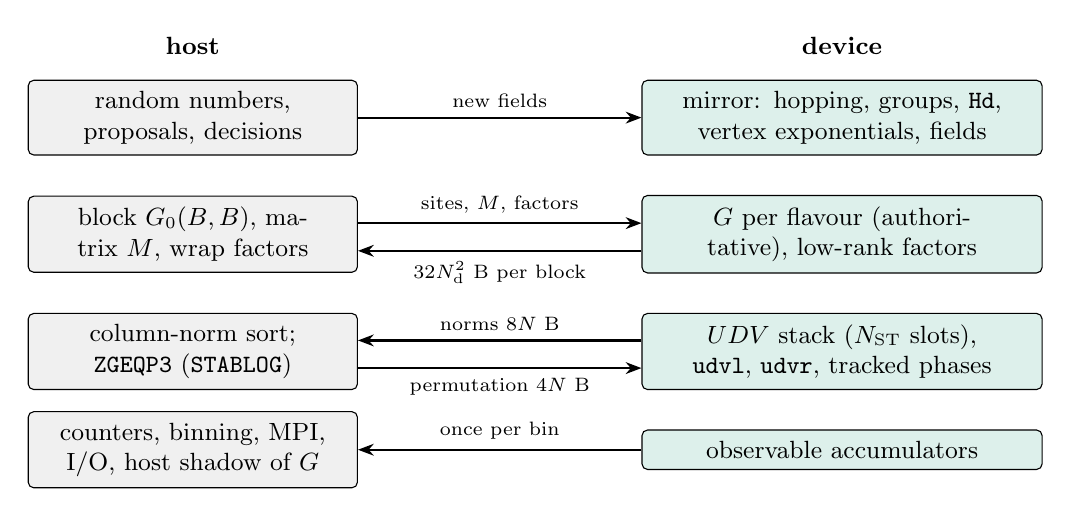
\begin{tikzpicture}[node distance=0.5cm and 0.6cm]
\node[devbox, text width=4.8cm] (mir) {mirror: hopping, groups, \texttt{Hd}, vertex exponentials, fields};
\node[devbox, text width=4.8cm, below=of mir] (g) {$G$ per flavour (authoritative), low-rank factors};
\node[devbox, text width=4.8cm, below=of g] (st) {$UDV$ stack ($N_{\rm ST}$ slots), \texttt{udvl}, \texttt{udvr}, tracked phases};
\node[devbox, text width=4.8cm, below=of st] (acc) {observable accumulators};
\node[hostbox, text width=3.9cm, left=3.6cm of mir] (rng) {random numbers, proposals, decisions};
\node[hostbox, text width=3.9cm, left=3.6cm of g] (blk) {block $G_0(B,B)$, matrix $M$, wrap factors};
\node[hostbox, text width=3.9cm, left=3.6cm of st] (sort) {column-norm sort; \texttt{ZGEQP3} (\texttt{STABLOG})};
\node[hostbox, text width=3.9cm, left=3.6cm of acc] (obs) {counters, binning, MPI, I/O, host shadow of $G$};
\node[above=0.2cm of rng, font=\small\bfseries] {host};
\node[above=0.2cm of mir, font=\small\bfseries] {device};
\draw[arr] ([yshift=4pt]blk.east) -- node[above, font=\scriptsize]{sites, $M$, factors} ([yshift=4pt]g.west);
\draw[arr] ([yshift=-6pt]g.west) -- node[below, font=\scriptsize]{$32\Nd^2$ B per block} ([yshift=-6pt]blk.east);
\draw[arr] ([yshift=4pt]st.west) -- node[above, font=\scriptsize]{norms $8N$ B} ([yshift=4pt]sort.east);
\draw[arr] ([yshift=-6pt]sort.east) -- node[below, font=\scriptsize]{permutation $4N$ B} ([yshift=-6pt]st.west);
\draw[arr] (acc.west) -- node[above, font=\scriptsize]{once per bin} (obs.east);
\draw[arr] (rng.east) -- node[above, font=\scriptsize]{new fields} (mir.west);
\end{tikzpicture}
\caption{Where the data live during a sweep, and what crosses the bus (production path). Grey: host; green: device.}
\label{fig:flow}
\end{figure}


\subsection{How residency is expressed}

All device data are Fortran module allocatables with a host twin of the same name. Residency is expressed with OpenMP data directives only (\file{gpu\_state\_mod.F90:1165-1206}):
\begin{itemize}
\item \texttt{!\$omp target enter data map(to: ...)} once at setup for the constant mirror (the model), which copies the host values to newly allocated device memory;
\item \texttt{!\$omp target enter data map(alloc: ...)} for work arrays, which allocates device memory without a copy;
\item \texttt{!\$omp target update to(...)} and \texttt{from(...)}, often on array sections, for the transfers during the run;
\item \texttt{!\$omp target exit data map(delete: ...)} at the end.
\end{itemize}
Kernels are \texttt{!\$omp target teams distribute parallel do} loops over these arrays; the OpenMP runtime finds the device copy because the array is present. \texttt{alf\_la} obtains device addresses with \texttt{use\_device\_addr}. There is no \texttt{is\_device\_ptr}, \texttt{omp\_target\_alloc} or unified memory anywhere in \file{Prog/gpu\_*.F90}. Arrays are passed to kernels as explicit-shape dummy arguments: ifx copies the descriptors of module allocatables that are referenced inside a target region at every launch (16.0 against 10.7~$\mu$s per launch, \file{gpu\_lowrank\_mod.F90:1364-1366}). % gpu_lowrank_mod.F90 comment

\subsection{The constant mirror of the model}

Built on the host in \texttt{gpu\_state\_setup} (\file{gpu\_state\_mod.F90:620-703}) and uploaded once. Table~\ref{tab:mirror} lists it.

\begin{small}
\begin{longtable}{@{}p{2.9cm}p{3.6cm}p{8.4cm}@{}}
\caption{The constant device mirror (\file{gpu\_state\_mod.F90:40-97, 146-172}). $n_{\rm el}$: number of active hopping elements; $n_d$: number of sites of an element; $N_{\rm op}$: number of vertices per slice.}\label{tab:mirror}\\
\toprule
Array & Shape, type & Content \\
\midrule\endfirsthead
\toprule Array & Shape, type & Content \\ \midrule\endhead
\texttt{hop\_start} & $\NFL+1$, int & first element of each flavour \\
\texttt{hop\_meta} & $(4,n_{\rm el})$, int & kind (1 real, 2 complex), $n_d$, offset into site list, offset into matrices \\
\texttt{hop\_P} & $\sum n_d$, int & site list $P$ of each element \\
\texttt{hop\_Rval} & $\sum 4n_d^2$, real(8) & for real elements: $e^{-\dt T_e}$, its inverse, and the half steps for \texttt{Symm} (\texttt{mat}, \texttt{invmat}, \texttt{mat\_1D2}, \texttt{invmat\_1D2}) \\
\texttt{hop\_Cval} & $\sum 4n_d^2$ + td part, complex & the same for complex elements, followed by one matrix per (time-dependent element, slice, kind) \\
\texttt{hop\_gptr} & $n_{\rm groups}+1+n_{\rm td}$, int & checkerboard groups: start of each group in the element list \\
\texttt{hop\_aux} & $(2,n_{\rm el})$, int & offset into the dense copies, flag ``$P$ is the identity'' \\
\texttt{hop\_At}, \texttt{hop\_Ac} & $4n_d^2$ per dense element & transposed real and complex copies of dense ($n_d>8$) elements, for the left-multiply variants \\
\texttt{V\_meta} & $(4,N_{\rm op},\NFL)$, int & $N$ of the vertex, offset into sites, offset into exponentials, skip flag ($|g|<\epsilon$) \\
\texttt{V\_type} & $N_{\rm op}$, int & field type (1 Ising, 2 four-valued) \\
\texttt{V\_P} & $\sum N$, int & sites of each vertex \\
\texttt{V\_exp} & $\sum N(2t+1)$, complex & the table \texttt{E\_exp}$(i,s)$, $s=-t\ldots t$, of the exponentials $e^{g\eta(s)V}$ \\
\texttt{vr\_ptr}, \texttt{vr\_ent} & $(N+1,\NFL)$, $(2,\cdot)$ & for each site $r$, the list of (vertex, position) pairs in ALF's operator order; used by the fused slice kernels \\
\texttt{nsigma\_d} & $(N_{\rm op},\Lt)$, complex & the auxiliary field; kept current during the sweep \\
\texttt{nsigma\_t} & $N_{\rm op}$, int & field type per vertex \\
\bottomrule
\end{longtable}
\end{small}

Three details matter for exact agreement with the CPU:
\begin{itemize}
\item For real elements the lower triangle is filled from the upper one, as ALF's symmetric multiply routines read only the upper triangle; real elements with $n_d>8$ keep the full stored matrix, because ALF's \texttt{ZLARCM} uses all of it (\file{gpu\_state\_mod.F90:765-778}).
\item For complex elements with $n_d>8$ the imaginary part of the diagonal is set to zero, as \texttt{ZHEMM} ignores it (lines 779-786).
\item Inactive elements ($|g|^2\le$ \texttt{Zero}) are not stored, as the host skips them.
\end{itemize}
Host-only tables: \texttt{hop\_gstart}, \texttt{hop\_big} and, for time-dependent hopping, \texttt{td\_grp}$(\Lt,2,n_{\rm td,max},\NFL)$ and \texttt{td\_n}. These select which group a kernel launch processes and need not be on the device.

\dis{ADR-002 (section 2) describes arrays \texttt{cb\_idx}, \texttt{cb\_exp} (bond pairs and $2\times2$ exponentials), \texttt{T\_exp}$(N,N,F,4)$, \texttt{V\_site} and \texttt{rnd\_d}. None exists. The code uses a general element list with blocks of any size $n_d$, checkerboard groups and dense copies, and time-dependent hopping, which the ADR does not cover.}

\subsection{Work arrays}

\begin{small}
\begin{longtable}{@{}p{3.3cm}p{4.0cm}p{7.6cm}@{}}
\caption{Device work arrays. $N_{\rm ST}$: stabilisation slots (\texttt{NSTM}); $F$: $\NFL$; $F_e$: $N_{\rm FL,eff}$. All mapped with \texttt{map(alloc:)}.}\label{tab:work}\\
\toprule
Array (module) & Shape & Mirrors / role \\
\midrule\endfirsthead
\toprule Array (module) & Shape & Mirrors / role \\ \midrule\endhead
\texttt{G\_d} (state) & $(N,N,F)$ & \texttt{GR}; authoritative copy of $G$ \\
\texttt{udv\_U}, \texttt{udv\_V} (state) & $(N,N,N_{\rm ST},F_e)$ & the stack \texttt{udvst}: $U$ and $V$ of each stabilisation point \\
\texttt{udv\_D} / \texttt{udv\_L} & $(N,N_{\rm ST},F_e)$ & scales: complex $D$ (default) or real $\log D$ (\texttt{STABLOG}); the other is a $1\times1\times1$ dummy \\
\texttt{udw\_U}, \texttt{udw\_V} & $(N,N,2,F_e)$ & slot 1 = \texttt{udvl}, slot 2 = \texttt{udvr} \\
\texttt{udw\_D} / \texttt{udw\_L} & $(N,2,F_e)$ & their scales \\
\texttt{GT0\_d}, \texttt{G0T\_d}, \texttt{GTT\_d} & $(N,N,F)$ & only with \texttt{Ltau=1}: $G(\tau,0)$, $G(0,\tau)$, $G(\tau,\tau)$ \\
\texttt{scr\_c}, \texttt{scr\_vec}, \texttt{scr\_r}, \texttt{scr\_ipiv}, \texttt{scr\_work} & $(N,N,2)$, $(N,4)$, $(N,2)$, $N$, $64N+64$ & scratch; \texttt{scr\_vec(:,1:2)} holds the rank-one vectors \\
\texttt{Hd} (wrap) & $(N,N,F,4)$ & precomputed dense hopping products, only for $N\le800$ (Section~\ref{sec:wrap}) \\
\texttt{sA}, \texttt{sB}, \texttt{sC}, \texttt{st\_Gn}, \texttt{st\_Gt} (stab) & $(N,N)$ each & stabilisation scratch, new and wrapped $G$ \\
\texttt{st\_tau}, \texttt{st\_Dl}, \texttt{st\_nrm}, \texttt{st\_ipvt}, \ldots & $N$ & Householder scalars, scales, norms, pivots \\
\texttt{st\_dw}, \texttt{st\_dv} & $(2,F_e)$, $(N_{\rm ST},F_e)$ & tracked phases $\det U/|\det U|$ of the work slots and the stack \\
\texttt{t\_H1}, \texttt{t\_H2}, \texttt{t\_Q}, \texttt{t\_A}, \texttt{t\_B} (tau) & $(2N,2N)$ & \texttt{CGR2\_2} work; $Q$, $A$, $B$ only with the Newton--Schulz step \\
\texttt{G00\_d}, \texttt{t\_GR}, \texttt{t\_old}, \texttt{t\_S} (tau) & $(N,N,F)$, $(N,N,F)$, $(N,N,3)$, $(N,N,4)$ & $G(0,0)$, reference copy, previous values for the precision check \\
\texttt{X\_d}, \texttt{Y\_d} (lowrank) & $(N,\Nd,F)$ & low-rank factors; \texttt{Y\_d} only for the delayed scheme \\
\texttt{gbd}, \texttt{cbuf}, \texttt{bsd}, \texttt{bS\_d} (lowrank) & $(\Nd,\Nd,2)$, $(2\Nd+\Nd^2)\cdot 2$, \ldots & block-mode buffers (Section~\ref{sec:updates}) \\
\texttt{acc}, \texttt{acc0}, \texttt{tacc}, \texttt{tacc0}, \texttt{lacc1}, \texttt{lacc2} (obs) & per observable & accumulators of the device observables \\
\bottomrule
\end{longtable}
\end{small}

\subsection{Memory footprint}

Summing the shapes (complex numbers are 16 bytes) gives, per run,
\begin{equation}
M \approx 16N^2\Bigl[\underbrace{4N_{\rm ST}}_{\text{stack }U,V\;(F_e=2)} + \underbrace{2}_{G} + \underbrace{8}_{\rm udw} + \underbrace{2}_{\rm scr} + \underbrace{5}_{\rm stab} + \underbrace{16}_{\text{dense hop}} + \underbrace{8}_{\texttt{Hd}} \Bigr] + O(N N_{\rm ST}) .
\end{equation}
The dense hopping term is $\texttt{hop\_Rval}+\texttt{hop\_At}+\texttt{hop\_Ac}$, about $128N^2$ bytes per flavour. The bracket without the stack is 41, which agrees with the empirical rule of \file{TUNING\_DEFECT.md}, % TUNING_DEFECT.md "Memory"
\begin{equation}
M_{\rm peak} \approx (4N_{\rm ST}+40)\cdot16N^2\ \text{bytes} + 0.3~\text{GB (CUDA context)},
\end{equation}
which was checked at $L=48$, $\beta=48$ (19.7~GB predicted, 19.6~GB measured) and $L=32$ (2.8 predicted, 3.1 measured). % TUNING_DEFECT.md
With \texttt{Ltau=1} the $\tau$ pass adds about $480N^2+32N^2F$ bytes. The stack dominates: it grows as $N^2\Lt/\texttt{Nwrap}\propto L^5/\texttt{Nwrap}$ at $\beta\propto L$. This is why \texttt{Nwrap}=5 costs 45\,\% more memory than \texttt{Nwrap}=10 at $L=24$ (1553 against 1069 MiB, \file{TUNING\_DEFECT.md}). % TUNING_DEFECT.md Nwrap table
The host does not mirror the stack; the resident set of the host process at $L=36$ was 1.9~GB while the device held 5.2~GB (\file{TUNING\_DEFECT.md}). % TUNING_DEFECT.md

The code prints the size of every \texttt{gpu\_state} array and their total into the \texttt{info} file (\texttt{report\_layout}, \file{gpu\_state\_mod.F90:1223-1271}). That total does not include the arrays of the other modules.

\subsection{All host--device transfers in one sweep}

Table~\ref{tab:transfers} is the complete list for the production path (device updates in submatrix block mode, device stabilisation, device observables, \texttt{Ltau=0}), assembled from the code. Sizes are in bytes.

\begin{small}
\begin{longtable}{@{}p{3.6cm}p{2.9cm}p{3.4cm}p{4.9cm}@{}}
\caption{Host--device transfers per sweep, production path. $b\le\Nd$: vertices in a block; $k$: pending sites at a flush.}\label{tab:transfers}\\
\toprule
When & Direction & Size & What and where \\
\midrule\endfirsthead
\toprule When & Direction & Size & What and where \\ \midrule\endhead
per proposal & -- & 0 & nothing; decided from the host block (\file{gpu\_lowrank\_mod.F90:1693-1720}) \\
per block, begin & H$\to$D & $8\Nd$ & block sites \texttt{bsd} \\
per block, begin & D$\to$H & $32\Nd^2$ & block $G_0(B,B)$ for 2 flavours, \texttt{gbd}; 32~KB at $\Nd=32$ \\
per block, end & H$\to$D & $32(2\Nd+\Nd^2)$ & \texttt{cbuf}: wrap factors and packed $M$; 34.8~KB at $\Nd=32$ \\
per block, end & H$\to$D & $8\Nd$, $16b$ & pending sites \texttt{bS\_d}; new fields \texttt{nsigma\_d(vmin:vmax,t)} \\
per slice & -- & 0 & $G$ is not moved (\texttt{g\_in} is a no-op, \texttt{g\_out} sets a flag) \\
per decompose (each flavour) & D$\to$H, H$\to$D & $8N$, $4N$ & column norms, permutation (\texttt{la\_qrpp}) \\
per decompose & D$\to$H & 24 & scale test (\texttt{dev\_testscale}) \\
per \texttt{CGR} & D$\to$H, H$\to$D & $8N$, $4N$ & \texttt{la\_qrpp} of the middle matrix \\
per \texttt{CGR} & D$\to$H & 16 + 32 & phase; precision numbers (max, sum, two NaN counts) \\
per \texttt{CGR} (\texttt{STABLOG}) & D$\to$H, H$\to$D & $16N^2$, $16N^2+20N$ & \texttt{la\_geqp3\_host} \\
per measurement & D$\to$H & 3 reductions & kinetic, potential energy, density \\
per bin & D$\to$H, H$\to$D & size of accumulators & \texttt{gpu\_obs\_flush}: download, zero, upload \\
amortised & D$\to$H & $4\times$ slots & \texttt{info} slots of \texttt{alf\_la} \\
\bottomrule
\end{longtable}
\end{small}

At $L=24$ and $\Nd=32$ there are 8\,640 blocks per sweep (18 per slice $\times$ 480 slices) and 43\,200 copies, four H$\to$D and one D$\to$H per block (\file{p7/NOTES.md}, line 94). % p7/NOTES.md
Before block mode, the per-proposal transfers dominated: on the A30 at $N=400$ there were 432\,000 stream synchronisations and 46\,000 small D$\to$H copies per run of six sweeps, and the kernels ran only 1.4~s out of 24~s (\file{DELAYED\_SUBMATRIX.md}). % DELAYED_SUBMATRIX.md lines 45-46

Other paths add transfers: a host observable needs $16N^2$ per flavour and measured slice (\texttt{gpu\_g\_host}); the standard rank-one update needs 16 bytes of $G_{pp}$ per proposal and flavour and 16 bytes of field per acceptance; the $\tau$ pass with host observables needs $3\cdot16N^2$ per slice and flavour. With \texttt{Ltau=1}, \file{main.F90:1301} downloads $G$ once before every $\tau$ pass even when the pass runs entirely on the device.

\dis{The info line of \file{gpu\_update\_mod.F90:109} still says ``INTERIM per-slice G copies''; lines 52-53 of the same file and the code say that $G$ is device-authoritative and never copied per slice.}

\section{Propagation on the device}
\label{sec:wrap}

The propagation routines are in \file{Prog/gpu\_wrap\_mod.F90} (2660 lines). They reproduce the routines of \file{Hop\_mod.F90} and \file{Operator\_mod.F90} on device matrices, in the same order of factors, so that the device result agrees with the CPU to rounding.

\subsection{Hopping: five routines, three code paths}

ALF applies $e^{\pm\dt T}$ through five routines that differ in side (left or right multiplication), matrix (exponential or inverse) and the order of the elements. The device versions are listed in Table~\ref{tab:hop}.

\begin{table}[h]
\centering\small
\caption{Device hopping routines (\file{gpu\_wrap\_mod.F90:117-173}). ``left'' acts on the rows of $M$, ``right'' on its columns. Matrix index $k$: 1 $e^{-\dt T}$, 2 inverse, 3 and 4 half steps for \texttt{Symm}.}
\label{tab:hop}
\begin{tabular}{@{}lllll@{}}
\toprule
Device routine & ALF routine & Side & $k$ & Element order \\
\midrule
\texttt{gpu\_mmthr} & \texttt{Hop\_mod\_mmthr} & left & 1 & descending \\
\texttt{gpu\_mmthr\_m1} & \texttt{Hop\_mod\_mmthr\_m1} & left & 2 & ascending \\
\texttt{gpu\_mmthl} & \texttt{Hop\_mod\_mmthl} & right & 1 & ascending \\
\texttt{gpu\_mmthlc} & \texttt{Hop\_mod\_mmthlc} & left & 1 & ascending \\
\texttt{gpu\_mmthl\_m1} & \texttt{Hop\_mod\_mmthl\_m1} & right & 2 & descending \\
\bottomrule
\end{tabular}
\end{table}

\paragraph{(a) Dense precomputed product (\texttt{Hd}).} For $N\le\texttt{HOPD\_NMAX}=800$ (\file{gpu\_wrap\_mod.F90:104}) each of the four hopping sequences used in the sweep is applied once at setup to the identity. The result is a dense $N\times N$ matrix per flavour and sequence, \texttt{Hd}$(N,N,\NFL,4)$ (\texttt{hopd\_build}, lines 262-285). Applying a sequence is then one \texttt{la\_gemm} into scratch plus a copy kernel (lines 287-303). The comment at lines 252-254: ``applying one is a GEMM plus a copy instead of one launch per checkerboard group. Used for Ndim $\le$ HOPD\_NMAX; above that the group kernels are cheaper.'' This path is used regardless of the \texttt{Checkerboard} flag. For the production model the static hopping is dense anyway. \texttt{gpu\_mmthlc} has no \texttt{Hd} variant, so \texttt{WRAPUL} uses the group kernels.

Mathematically $\texttt{Hd}=\prod_e B_e$ is the same matrix as the product of the elements; numerically it differs from applying the elements one by one in the rounding of the product, at the level of $10^{-16}$ relative per application.

\paragraph{(b) Checkerboard groups.} When all elements have $n_d\le8$ sites, consecutive elements whose site lists are pairwise disjoint are combined into a \emph{group} (\file{gpu\_state\_mod.F90:66-73}). Elements of a group commute, so one kernel launch can apply all of them in parallel. For the square lattice with nearest-neighbour hopping there are four groups, so one $B_T$ costs four launches. The kernels are \texttt{k\_cb\_left\_g} and \texttt{k\_cb\_right\_g} (lines 638-669):
\begin{itemize}
\item \texttt{k\_cb\_left\_g}: \texttt{target teams distribute parallel do collapse(2)} over (column tile, element). Each thread handles \texttt{gpu\_tl} consecutive columns (default 1) and computes, for its element $e$ and column $j$, the $n_d$ new values $M_{P_e(i),j}\leftarrow\sum_l (B_e)_{il}M_{P_e(l),j}$.
\item \texttt{k\_cb\_right\_g}: the same over (element, row tile), \texttt{gpu\_tr}=2 rows per thread by default, ``tuned on the A30''.
\end{itemize}
The inner sums are written out by hand for $n_d=1$ (a scale), $n_d=2$ (an explicit $2\times2$) and general $n_d\le8$ (the element is gathered into a local array \texttt{w(8)}), in the order $l=1\ldots n_d$ of ALF's \texttt{ZDSLSYMM} and \texttt{ZSLHEMM} (\texttt{el\_left\_d}, \texttt{el\_right\_d}, lines 479-633). Real elements are applied with real arithmetic on the real and imaginary parts of $M$ separately, as ALF does.

A variant that applied all groups in one launch with a barrier between groups was removed in ticket 205: ``slower on the A30 and wrong on the Arc B580'' (lines 47-51).

\paragraph{(c) Dense elements ($n_d>8$).} If the site list is not the identity, the rows (or columns) are gathered into scratch, multiplied, and scattered back (\texttt{dense\_left}, \texttt{dense\_right}, lines 674-741). Complex elements use \texttt{la\_gemm}. For a real element times a complex matrix ALF uses \texttt{ZLARCM}; the device uses \texttt{la\_gemm\_cr}, which views the complex matrix as a real matrix of twice the height and calls one DGEMM:
\begin{equation}
M B \;\text{with $B$ real}:\quad \begin{pmatrix}\Re M\\ \Im M\end{pmatrix}_{\text{interleaved}} B ,
\end{equation}
which costs half the flops of a ZGEMM. For a left multiplication $BM$ the interleaving does not work directly. Two modes exist (\texttt{gpu\_dense\_left\_mode}, line 95; automatic: mode 1 for $n_d\le400$, mode 2 above, line 687): mode 1 multiplies with a complex copy \texttt{hop\_Ac} (four times the flops), mode 2 transposes, uses $(BM)^T=M^TB^T$ with \texttt{hop\_At} and \texttt{la\_gemm\_cr}, and transposes back.

\subsection{Time-dependent hopping (the point defect)}

The point defect is a hopping element whose coupling depends on the slice, $g_t(\tau)$ (\file{TIMEDEP\_HOPPING.md}). The element is $A(g)=U e^{gE}U^\dagger$. Instead of uploading a new matrix per slice, setup appends ordinary complex elements to the mirror, one per active slice and kind (\file{gpu\_wrap\_mod.F90:117-120, 176-212}):
\begin{itemize}
\item propagation: $A(g_t)$ as $k=1$ and $A(-g_t)$ as $k=2$;
\item \texttt{Symm}: $A(\bar g/2)$ and $A(-\bar g/2)$ as $k=3,4$, with $\bar g$ the average of $g_t(\tau)$ and $g_t(\tau-1)$.
\end{itemize}
Each sits in a group of its own. The host table \texttt{td\_grp}$(\tau,\text{kind},j,f)$ names the group to launch, 0 meaning inactive. Since $E$ has a single non-zero eigenvalue for the defect, the support reduction \texttt{td\_reduce} stores only the rows where eigenvectors with $E_k\ne0$ are non-zero (relative threshold $10^{-13}$): one site. Without it the set of matrices at $L=32$ would need more than 2~GB; \texttt{gpu\_supported} refuses sets above 2~GB (\file{gpu\_state\_mod.F90:601-602}).

Because time-dependent elements are the last of their flavour (\texttt{gpu\_supported} requires this), they are applied first in the descending routines and last in the ascending ones, around the static \texttt{Hd} product.

\subsection{Interaction vertices}

Each vertex $\Op_V(n)$ of the Hubbard model acts on one site $p_n$. Its exponential for field value $s$ is the diagonal factor \texttt{E\_exp}$(1,s)$, stored in \texttt{V\_exp}. The field is read on the device as $s=\mathrm{nint}(\Re\,\texttt{nsigma\_d}(n,\tau))$.

\begin{itemize}
\item \texttt{gpu\_Vop\_R}, \texttt{gpu\_Vop\_L} (lines 856-917): \texttt{Op\_mmultR} and \texttt{Op\_mmultL} for one vertex: scale rows (or columns) $P(i)$.
\item \texttt{gpu\_Vop\_wrap} (lines 921-963): \texttt{Op\_Wrapup}/\texttt{Op\_Wrapdo}: rows by $E(i,\pm s)$, then columns by $E(i,\mp s)$.
\item \texttt{k\_vslice\_R}, \texttt{k\_vslice\_L} (lines 980-1124): all vertices of a slice in one launch. Threads run over (column block of \texttt{gpu\_vb}=8 columns, row $r$). For row $r$ all vertices containing $r$ are applied in ALF's order through \texttt{vr\_ptr}/\texttt{vr\_ent}. Up to four factors per row are precomputed per thread. ``the same product sequence as the loop of calls'' (lines 966-968).
\item \texttt{k\_vwrap\_all} (lines 1137-1190): the whole-slice wrap in one launch; row and column factors are merged in operator order.
\item \texttt{k\_site\_wrap} (\file{gpu\_update\_mod.F90:280-298}): the single-site wrap used inside the update loop:
\begin{equation}
G_{rj}\leftarrow z_a G_{rj},\; G_{jr}\leftarrow z_b G_{jr}\;(j\ne r),\qquad G_{rr}\leftarrow z_b(z_a G_{rr}),
\end{equation}
with $z_a=$ \texttt{V\_exp}$(\cdot,\,{\rm dir}\cdot s)$ and $z_b=$ \texttt{V\_exp}$(\cdot,-{\rm dir}\cdot s)$. The diagonal is scaled row first, then column, ``ALF's \texttt{ZSCAL} order''.
\end{itemize}
In the sweep the wrap of $G$ cannot use the fused slice kernels: wraps and updates alternate vertex by vertex. In the delayed and submatrix schemes the per-vertex wrap is not applied to the device $G$ at all but folded into the low-rank representation (Section~\ref{sec:updates}).

\subsection{Composite operations}

\begin{itemize}
\item In the sweep (\file{gpu\_update\_mod.F90:470-629}): \texttt{gpu\_wrapgrup} applies \texttt{gpu\_mmthr} and \texttt{gpu\_mmthl\_m1} to $G$, i.e.\ $G\leftarrow e^{-\dt T}Ge^{\dt T}$, then loops over the vertices with wrap and update. \texttt{gpu\_wrapgrdo} does the updates first, then \texttt{gpu\_mmthl} and \texttt{gpu\_mmthr\_m1}.
\item For the stabilisation (\file{gpu\_wrap\_mod.F90:1196-1217}): \texttt{gpu\_wrapur\_slices} applies, for $\tau=\tau_1+1\ldots\tau_2$, \texttt{gpu\_mmthr} then \texttt{gpu\_Vslice\_R}, i.e.\ $U\leftarrow B_\tau U$. \texttt{gpu\_wrapul\_slices} applies the conjugate factors in reverse order for the left side.
\item \texttt{Symm} (\texttt{gpu\_symm}, lines 217-249): groups in descending order, half steps $k=3$ from the left and $k=4$ from the right. For the measurements \texttt{gpu\_symm\_build} (lines 360-390) forms the static matrices $A$ and $B$ once, so that $\mathrm{Symm}(G)=AGB$ is two GEMMs; \texttt{gpu\_symm\_td} adds the time-dependent half steps, $A(A_{td}GB_{td})B$.
\end{itemize}
The flavour loop is on the host: \texttt{do nfe=1,N\_FL\_eff; nf=Calc\_Fl\_map(nfe)}. There is no batching over flavours.

\dis{The header of \file{gpu\_wrap\_mod.F90} (line 37) says ``Nothing in the sweep calls these yet''; the routines are called by the update, stabilisation, $\tau$ and observable modules. \file{HARD.md} plans ``one kernel per checkerboard family'' and ``both flavours per launch''; the code launches per group, loops over flavours on the host, and uses the dense \texttt{Hd} product for $N\le800$ even with checkerboard hopping.}

\subsection{Operation counts}

The following counts are derived from the code, not measured. Per slice and flavour:
\begin{itemize}
\item \texttt{Hd} path, $G\leftarrow BGB^{-1}$: 2 ZGEMMs of size $N$, $2\times8N^3$ real flops, plus two copies of $N^2$. At $N=576$ this is 3.1~GFlop per slice and flavour, or about 2.9~TFlop per sweep ($2\Lt=480$ slices, 2 flavours). At the FP64 peak of an A30 (about 10~TFlop/s with tensor cores according to the vendor data sheet, not measured here) that alone is at least 0.3~s of the 5.25~s sweep.
\item Checkerboard path, square lattice: about $2N$ bonds, each $2\times2$ on $N$ columns, about $24N^2$ flops per $B_T$ in four launches.
\item Vertex wraps: $N_{\rm op}=N$ single-site launches of $2N$ complex multiplications each, i.e.\ $O(N^2)$ work in $N$ launches. These launches are the reason for the block mode of Section~\ref{sec:updates}.
\item \texttt{WRAPUR} per slice: 1 ZGEMM (or 4 group launches) plus 1 fused vertex launch.
\end{itemize}
The kernel benchmark of Phase~1 on the A30 gives the scale (\file{BENCHMARKS.md}): a dense $B_T$ product takes 53, 172 and 2757~$\mu$s at $N=144$, 400, 1024 on the device against 1095, 22\,941 and 388\,561~$\mu$s on one host core; the vertex wrap with one launch per site took 1621~$\mu$s at $N=144$ (host 199~$\mu$s), and fused into one launch 13~$\mu$s (host 36~$\mu$s). % BENCHMARKS.md Phase 1
The last pair shows the problem of launch latency in one number: a fused kernel is 125 times faster than one launch per site.

\section{Stabilisation on the device}
\label{sec:stab}

The stabilisation is in \file{Prog/gpu\_stab\_mod.F90} (2118 lines). It replaces \texttt{WRAPUR}, \texttt{WRAPUL}, the stack handling of \file{main.F90}, \texttt{CGR} and \texttt{Control\_PrecisionG}. On the device the full sequence runs without moving any $N\times N$ matrix to the host (in the default stabilisation).

\subsection{Stacks and slots}

The stack \texttt{udvst} of ALF becomes \texttt{udv\_U}, \texttt{udv\_V}, \texttt{udv\_D} (or \texttt{udv\_L} for \texttt{STABLOG}) with one slot per stabilisation point and flavour. The two working decompositions \texttt{udvl} and \texttt{udvr} are slots 1 and 2 of \texttt{udw\_*}. The exchanges of \file{main.F90} (``\texttt{udvl = udvst(NST)}; \texttt{udvst(NST) = udvr}'' on the way up, the mirror image on the way down) are device-to-device copies (\texttt{gpu\_stab\_exchange}, \file{gpu\_stab\_mod.F90:350-414}). The tracked phases of $\det U$ (\texttt{st\_dw}, \texttt{st\_dv}) travel with the slots. Only the CPU $\tau$ pass needs the stack on the host; then \texttt{udvst} is downloaded on the way down.

The calls in \file{main.F90} (lines 706-1294) follow the CPU code one to one: \texttt{gpu\_stab\_wrapul} with \texttt{gpu\_stab\_store\_l} builds the initial left stack, \texttt{gpu\_stab\_cgr} computes the initial $G$, and in the sweep \texttt{gpu\_stab\_wrapur}/\texttt{wrapul}, \texttt{gpu\_stab\_exchange} and \texttt{gpu\_stab\_cgr} replace their CPU counterparts at each stabilisation point. \texttt{Op\_phase}, the phase product and \texttt{Control\_PrecisionP} stay on the host; they need only scalars.

\subsection{The QR decomposition with pre-pivoting}
\label{sec:qrpp}

\paragraph{The problem.} ALF factorises with \texttt{ZGEQP3}, the QR decomposition with column pivoting. At step $j$ it chooses, among the remaining columns, the one with the largest norm \emph{of its component orthogonal to the columns already chosen}, and updates those partial norms after each step. That makes every step depend on the previous one and on a global maximum: it is a sequence of matrix--vector operations and cannot be blocked into matrix products. No GPU library offers it: cuSOLVER and oneMKL have none, and MAGMA's \texttt{zgeqp3} is bound by matrix--vector work and runs only on NVIDIA and AMD (\file{HARD.md}, section 2). Running \texttt{ZGEQP3} on the host would cost a transfer of the matrix both ways and the host time: about 5.7~s per \texttt{CGR2\_2} at $N=1024$, and 14~ms at $N=400$ and 186~ms at $N=1024$ for one \texttt{ZGEQP3} on one core (\file{HARD.md}; \file{ADR-001}, item 4). % HARD.md section 2; ADR-001 item 4

\paragraph{The solution: pre-pivoting.} \texttt{la\_qrpp} (\file{alf\_la\_mod.F90:1974-2065}) sorts the columns once, by their initial norms, in descending order, and then calls the unpivoted, blocked \texttt{la\_geqrf}:
\begin{enumerate}
\item \texttt{k\_colnorms}: the scaled 2-norm of every column, one device thread per column with a serial loop (fixed summation order, ticket 212);
\item D$\to$H of the $N$ norms; check for NaN or Inf;
\item on the host, a stable insertion sort in descending order, giving a permutation with the semantics of \texttt{ZGEQP3}'s \texttt{jpvt};
\item H$\to$D of the permutation; \texttt{k\_permute\_cols};
\item \texttt{la\_geqrf}.
\end{enumerate}
Why this suffices for ALF: before the decomposition the columns of $B\,U$ are multiplied by the scales $D$ of the previous decomposition (\texttt{k\_scale\_cols}). These scales span many orders of magnitude, so the initial column norms are already strongly graded, and the order that \texttt{ZGEQP3} would choose differs from the order of the initial norms only among columns of similar size. The scales $|R_{ii}|$ then come out in nearly descending order, which is what the stabilisation needs.

\paragraph{The comparison test.} Ticket 104 compared, on the CPU, ALF with \texttt{ZGEQP3} and ALF with pre-pivoting plus \texttt{ZGEQRF}, at the same seeds. For the default stabilisation the mean precision of $G$ stayed within $\pm5\,\%$ and the Monte Carlo trajectories were identical (\file{HARD.md}, section 2). For \texttt{STABLOG} the maximum deviation of $G$ became up to 14 times larger ($4.4\times10^{-6}\to6.2\times10^{-5}$ at $L=8$, $\beta=20$, $U=4$), with more ``Unstable matrix'' aborts at $U=8$. Ticket 108 tried a two-pass sort and a blocked re-ranking; both failed (outliers up to 4.6 times in the maximum and about 1.4 times higher means). Therefore \texttt{STABLOG} keeps the host \texttt{ZGEQP3} in \texttt{CGR} (\texttt{la\_geqp3\_host}). % HARD.md, ADR-001 item 4, ticket 108
The unit test \texttt{t\_qrpp} compares \texttt{la\_qrpp} with \texttt{QDRP\_decompose} called with all columns fixed after the same sort; the device and host norms can differ in the last bit, so columns with tied norms may be ordered differently, ``an equally valid pivot order'' (\file{alf\_la\_mod.F90:1980}). The CPU build (\texttt{GPU=none}) keeps \texttt{ZGEQP3} (owner decision at the Phase~1 gate, \file{PLAN.md}, section 5).

\subsection{Decompose (default stabilisation)}

\texttt{dev\_decompose} (\file{gpu\_stab\_mod.F90:489-583}) computes $U D V$ from $\tilde U = B(\tau_2,\tau_1)U_{\rm old}$ (already propagated) in these steps:
\begin{enumerate}
\item \texttt{k\_scale\_cols}: $\tilde U_{:,j}\leftarrow \tilde U_{:,j}\,D_j$.
\item \texttt{la\_qrpp}: $\tilde U P = QR$, Householder scalars $\tau_i$ in \texttt{st\_tau}.
\item \texttt{k\_diagabs}, \texttt{k\_divrows}: $D_i=|R_{ii}|$, $R_{ij}\leftarrow R_{ij}/|R_{ii}|$ for $j\ge i$ (so $R=D\tilde R$).
\item \texttt{Pivot\_phase} on the host: the sign of the permutation (from the pivot vector, no transfer of matrices).
\item \texttt{k\_phase}: one serial device loop computing the phase of $\prod_i \tilde R_{ii}$, and the phase of $\det Q$ from the $\tau_i$ (see below).
\item \texttt{k\_scale\_row1}: the first row of $\tilde R$ is divided by that phase; ``to set Det(R)=1 [=Det(V)]'' as the CPU code says (\file{udv\_state\_mod.F90:527}); step 10 multiplies the first column of $U$ by it, as the CPU does with \texttt{ZSCAL} (line 614).
\item Permute the old $V$ with the pivot vector (\texttt{ZLAPMR}/\texttt{ZLAPMT} equivalents), and form $V\leftarrow\tilde R\,V$ (right side) or $V\leftarrow V\tilde R^\dagger$ (left side) with \texttt{la\_gemm}; the triangular factor is multiplied as a full matrix.
\item Form $Q$ by applying it to the identity with \texttt{la\_ormqr} (not \texttt{la\_ungqr}, see below), copy to $U$.
\item Newton--Schulz step on $U$ (below).
\item \texttt{k\_scale\_col1}: $U_{:,1}\leftarrow U_{:,1}\cdot{\rm phase}$.
\item \texttt{dev\_testscale}: one D$\to$H of three numbers; a NaN scale is an error (``Switch to LOG is required''), $D_1>0.1\,\texttt{huge}$ or $D_N<10\,\texttt{tiny}$ gives a warning.
\end{enumerate}
The cost is about $37N^3$ real flops per decompose (\texttt{geqrf} $\tfrac{16}{3}N^3$, \texttt{ormqr} on $I$ $8N^3$, $\tilde RV$ $8N^3$, Newton--Schulz $16N^3$; derived from the code).

\paragraph{Why \texttt{ormqr} on the identity and a Newton--Schulz step.} With \texttt{la\_ungqr} the precision of $G$ in the sweep was 4 times (mean) and 11 times (max) worse than on the CPU at $N=36$; applying $Q$ to $I$ with \texttt{ZUNMQR} restored the CPU level at $N=36$, ``at N = 144 the Newton--Schulz step below is needed in addition'' (\file{gpu\_stab\_mod.F90:559-568}). The cause is that cuSOLVER's $Q$ is less orthogonal than LAPACK's: $\|Q^\dagger Q-I\|$ about $1.6\times10^{-14}$ against $3.3\times10^{-15}$ at $N=400$ (\file{DISCREPANCIES.md}). % DISCREPANCIES.md
One Newton--Schulz step,
\begin{equation}
Q \leftarrow Q\,\tfrac12\bigl(3I - Q^\dagger Q\bigr),
\end{equation}
reduces the orthogonality defect quadratically: with $Q^\dagger Q = I+\Delta$, the new $Q$ has $Q^\dagger Q = (I-\tfrac12\Delta)(I+\Delta)(I-\tfrac12\Delta) = I-\tfrac34\Delta^2+O(\Delta^3)$. It costs two GEMMs (\texttt{sA}$=U^\dagger U$, kernel \texttt{k\_ns} forming $-\tfrac12$\texttt{sA}$+\tfrac32I$, \texttt{sB}$=U\,$\texttt{sA}). Measured in ticket 206 ($12\times12$, $\beta=4$, same seeds): without the step, precision of $G$ mean $9.7\times10^{-11}$ and max $1.2\times10^{-6}$; with it $5.4\times10^{-11}$ and $3.8\times10^{-7}$; CPU $4.1\times10^{-11}$ and $7.2\times10^{-7}$ (\file{gpu\_stab\_mod.F90:565-568}). The step is on by default for all backends; \texttt{ALF\_GPU\_NS=0} switches it off (debug only). oneMKL's $Q$ does not need it, but it was kept for uniformity (\file{DECISIONS.md}, item 26).

\subsection{Decompose with \texttt{STABLOG}}

With \texttt{STABLOG} the scales are kept as $\log D$ (\file{gpu\_stab\_mod.F90:515-544}). \texttt{k\_lognorm} computes $\log\|\tilde U_{:,j}\|_2+L_j$ for every column, the host sorts with the CPU's selection sort (\texttt{sort\_stablog}, the same one-sided swap \texttt{tn(pvt)=tn(i)} as the CPU code), the permutation goes back, $U$, $V$ and $L$ are permuted on the device, and an unpivoted \texttt{la\_geqrf} follows. \texttt{k\_stablog\_scale} then applies $U_{ij}\leftarrow U_{ij}\,e^{L_j-L_i}$ for $j>i$ and $L_i\leftarrow\log|R_{ii}|+L_i$. Large and small scales exist only in logarithmic form.

\subsection{Assembling $G$ on the device (\texttt{CGR})}

\texttt{dev\_cgr} and \texttt{cgr\_solve} (\file{gpu\_stab\_mod.F90:869-958}) evaluate Eq.~\eqref{eq:cgr}:
\begin{align}
\texttt{sA} &= U_R^\dagger U_L, \qquad \texttt{sB} = V_R V_L,\\
T &= D_R\,(V_RV_L)\,D_L + U_R^\dagger U_L \qquad(\texttt{k\_tpup}: T_{ij}=D_{R,i}T_{ij}D_{L,j}+\texttt{sA}_{ij}),\\
G &= U_L\,T^{-1}\,U_R^\dagger .
\end{align}
With \texttt{STABLOG}, \texttt{k\_tpup\_log} implements the four sign cases of \file{cgr1\_mod.F90}, so that no exponential overflows; for example $T_{ij}=\texttt{sA}_{ij}+e^{L_{R,i}+L_{L,j}}T_{ij}$ when both logarithms are $\le0$ and $T_{ij}=e^{-L_{R,i}-L_{L,j}}\texttt{sA}_{ij}+T_{ij}$ when both are positive.

$T^{-1}$ is applied through a QR of $T$ with pre-pivoting, $TP=QR=QD\tilde R$, so $T^{-1}=P\tilde R^{-1}D^{-1}Q^\dagger$. For \texttt{NVAR=1}:
\begin{enumerate}
\item \texttt{sA}$\leftarrow U_R^\dagger$ (\texttt{k\_ct}); with \texttt{STABLOG} rows are scaled by $e^{-L}$ where $L>0$;
\item \texttt{la\_ormqr('L','C')}: $Q^\dagger\,\texttt{sA}$;
\item \texttt{k\_rowdiv}: divide row $i$ by $D_i$ (Smith's complex division in the HIP kernel);
\item \texttt{la\_trsm('L','U','N','N')} with $\tilde R$;
\item \texttt{k\_iperm\_rows}: undo $P$ (\texttt{ZLAPMR} backward);
\item $G = U_L\cdot(\ldots)$ with \texttt{la\_gemm}.
\end{enumerate}
\texttt{NVAR=2} works on $T^\dagger$ with right-side operations. The cost is about $41N^3$ flops per \texttt{CGR} (derived). The result \texttt{st\_Gn} is copied device-to-device into \texttt{G\_d}; in the ``lazy'' mode (ticket 208-1) the host $G$ is not written.

\subsection{Precision monitoring}

\texttt{Control\_PrecisionG} compares the wrapped $G$ with the fresh one. On the device (\texttt{dev\_prec}, \texttt{k\_prec}, \file{gpu\_stab\_mod.F90:743-754, 1524-1567}) one kernel computes
\begin{equation}
x_{\max}=\max_{ij}|G^{\rm wrap}_{ij}-G^{\rm new}_{ij}|,\quad x_{\rm sum}=\sum_{ij}|G^{\rm wrap}_{ij}-G^{\rm new}_{ij}|,
\end{equation}
and the number of NaN entries in each matrix (by a bit test, so that a NaN cannot hide in a comparison). The sum is in fixed order: one thread per column writes its column sum, then one thread adds the column sums. Four numbers go to the host, where \texttt{Control\_PrecisionG\_vals} (\file{control\_mod.F90:463-526}) does what the CPU routine does: abort on NaN, abort if $x_{\max}$ exceeds the threshold (default 10, settable with \texttt{ALF\_UNSTABLE\_THRESHOLD}), otherwise accumulate mean and maximum.

The production threshold was lowered to $10^{-4}$ after a faulty GPU tile produced corrupted Green functions with deviations of 10 to 28, while healthy runs stay between $10^{-10}$ and $3\times10^{-8}$ up to $L=44$ (\file{DECISIONS.md}, item 46). % DECISIONS.md 46
The run then restarts from the last configuration within the job (at most 10 times).

\subsection{The phase of the determinant}

The phase of the fermion determinant is tracked as in \file{cgr1\_mod.F90}. ALF computes it from two parts: the phase of $\det(U_R^\dagger U_L)$, obtained with an LU decomposition (\texttt{PHASE = CONJG(DET\_C(RHS))}, \file{cgr1\_mod.F90:303}), and the phase of $\det T$ from its QR factors.

\paragraph{Phase of $\det T$ from Householder scalars.} LAPACK represents $Q=H_1H_2\cdots H_n$ with $H_i=I-\tau_iv_iv_i^\dagger$, $v_i(i)=1$. By the matrix determinant lemma
\begin{equation}
\det H_i = 1-\tau_i\,v_i^\dagger v_i .
\end{equation}
$H_i$ is unitary: $H_i^\dagger H_i = I-(\tau_i+\bar\tau_i)v_iv_i^\dagger+|\tau_i|^2(v_i^\dagger v_i)\,v_iv_i^\dagger = I$, which requires $|\tau_i|^2\,v_i^\dagger v_i = 2\,\Re\tau_i$. Inserting,
\begin{equation}
\det H_i = 1-\frac{2\tau_i\Re\tau_i}{|\tau_i|^2} = \frac{|\tau_i|^2-2\tau_i\Re\tau_i}{|\tau_i|^2}.
\end{equation}
With $\tau_i=a+ib$ the numerator is $a^2+b^2-2a^2-2iab=-(a+ib)^2=-\tau_i^2$, so
\begin{equation}
\label{eq:dethi}
\det H_i = -\frac{\tau_i^2}{|\tau_i|^2} = -\frac{\tau_i}{\bar\tau_i}\qquad(\tau_i\ne0),\qquad \det H_i=1\quad(\tau_i=0).
\end{equation}
It has modulus one and does not depend on the normalisation of $v_i$; only the unitarity of $H_i$ is used. The same formula is in upstream \file{cgr1\_mod.F90:532-536}. The device kernel \texttt{k\_cgr\_phase} (\file{gpu\_stab\_mod.F90:1420-1452}) multiplies the phase by $R_{ii}/|R_{ii}|$ and by Eq.~\eqref{eq:dethi} for every $i$, and by the sign of the permutation. In code: \texttt{z = 1 - 2*(z/|z|)*(Re z/|z|)}, which is Eq.~\eqref{eq:dethi}.

\paragraph{The LU-free phase of $\det(U_R^\dagger U_L)$ (2026-11-13).} On the CPU, and still on NVIDIA and AMD, the device computes $\det(U_R^\dagger U_L)$ with \texttt{la\_getrf} on the product and \texttt{k\_det\_phase} (product of the diagonal, sign flip for each row interchange). That is an extra $N^3$ factorisation per \texttt{CGR}, and on Intel oneMKL's \texttt{getrf} is slow (13~ms at $N=1024$, \file{SPEEDUPS.md}). % SPEEDUPS.md section 4
Since $\det(U_R^\dagger U_L)=\overline{\det U_R}\,\det U_L$, it suffices to track the phase of $\det U$ for every stored $U$. Every $U$ is produced by a decompose, where $U = Q_{\rm ns}\,\mathrm{diag}(\phi,1,\ldots,1)$ and $Q_{\rm ns}=Q\cdot\tfrac12(3I-Q^\dagger Q)$. The Newton--Schulz factor is Hermitian positive definite, so its determinant is real and positive and does not change the phase. Hence
\begin{equation}
\frac{\det U}{|\det U|} = \phi\prod_i\Bigl(-\frac{\tau_i}{\bar\tau_i}\Bigr)\Big/\Bigl|\ldots\Bigr|,
\end{equation}
which \texttt{k\_phase} computes during the decompose at no extra cost (\file{gpu\_stab\_mod.F90:1024-1054}; line 1044 reads \texttt{if (a2 > 0) dq = dq*(1 - 2*z*(real(z)/a2))} with \texttt{a2}$=|z|^2$). The value is stored with the slot (\texttt{st\_dw}, \texttt{st\_dv}) and copied with it. In \texttt{CGR}, \texttt{k\_det\_phase\_u} forms $\det=\overline{d_R}\,d_L$ and the phase $\bar d/|d|$, replacing the LU (lines 1076-1086). Reset slots have $\det=1$. If a slot was loaded from the host (no tracked phase), the LU is used as fallback.

This path is enabled only with oneMKL (\texttt{\#if defined(ALF\_LA\_ONEMKL)}, lines 471-477). The comment in the code: ``enabled where it has been measured and verified: oneMKL (Max 1550, 2026-11-13: 4.45 $\to$ 4.04 s per sweep at L=24, phase equal to the LU phase to 6e-15). HIP: \texttt{hk\_phase} does not track det(U). CUDA: not yet run.'' \file{SPEEDUPS.md} gives $5.8\times10^{-15}$ and also 10.06$\to$9.59~s with default switches. % SPEEDUPS.md section 2
\texttt{ALF\_GPU\_CGR\_LU=2} runs both routes and reports the largest difference.

One caveat follows from the derivation: Eq.~\eqref{eq:dethi} holds for the LAPACK representation. If the own device QR (Section~\ref{sec:ownqr}) is used on Intel together with the LU-free phase, it must produce LAPACK-convention $\tau_i$; the own kernels do follow \texttt{ZLARFG} conventions (\file{alf\_la\_sycl\_devqr.hpp}), and the V7 measurements of 2026-11-13 used both together. \todo{a dedicated test of the LU-free phase with ALFSH\_DEVQR=2 is not documented separately from the V7 run}

\dis{The header of \file{gpu\_stab\_mod.F90} (lines 46-49) says that the phase comes ``from the determinant phases of the two U factors \ldots la\_getrf only as fallback''. In the code only the oneMKL backend tracks $\det U$; CUDA and HIP always use \texttt{la\_getrf}.}

\subsection{Vendor QR and own device QR}
\label{sec:ownqr}

\texttt{la\_geqrf} and \texttt{la\_ormqr} are the most frequent large operations: at $L=24$ about 217 calls per sweep (\file{alf\_hip\_qr.hip.cpp:3-4}). Their quality differs strongly between vendors:
\begin{itemize}
\item \textbf{cuSOLVER} is adequate: at $n=1024$ \texttt{geqrf} 7.8~ms, \texttt{ormqr} 2.2~ms, \texttt{getrf} 4.1~ms, together about 8\,\% of a sweep; a CUDA port of the own QR was therefore not made (\file{SPEEDUPS.md}, section 3). % SPEEDUPS.md
\item \textbf{oneMKL} \texttt{geqrf} is hybrid: it factorises each panel on the host CPU and updates the trailing matrix on the device. At $L=24$ this cost 2.4~s per sweep (\file{GPU\_PLAN\_V2.md}, section 2). % GPU_PLAN_V2 sec 2
\item \textbf{rocSOLVER} \texttt{zgeqrf}/\texttt{zunmqr} at $n=576$ launch about 2300 tiny kernels each, 8.8~ms per call, about 0.12~TFlop/s on an MI210; QR was 93\,\% of all kernel dispatches and about 44\,\% of the sweep (\file{alf\_hip\_qr.hip.cpp:3-4}; \file{GPU\_PLAN\_V2.md}). % alf_hip_qr.hip.cpp header
\end{itemize}

\paragraph{The own HIP QR} (\file{alf\_hip\_qr.hip.cpp}, 347 lines) is a blocked right-looking Householder QR in LAPACK conventions (\texttt{ZLARFG} reflectors, $R$ in the upper triangle, $v$ below with implied unit diagonal, $\tau$), so all consumers use its output unchanged.
\begin{itemize}
\item Panel kernel \texttt{k\_qr\_panel<NB,T,R>}: one work-group factorises the whole panel with the panel held in registers; row $i$ lives in thread $i \bmod T$. $NB=16$, $T=256$ threads for $m\le1024$; $NB=8$, $T=512$ for $m\le2304$. Per column: the norm by a wave-level sum plus one exchange through local memory, \texttt{ZLARFG}, then the dot products with the remaining panel columns (three barriers per column). No $T$ factor is formed.
\item Apply kernel \texttt{k\_apply\_left<Q,NV>}: one 64-lane wave owns $NV$ columns and applies the reflectors one after another (a dot product and a rank-one update per reflector). It does the trailing update of each panel in one launch and also implements \texttt{unmqr}. No compact-WY form and no GEMM.
\item Right-side \texttt{unmqr} is computed as $(Q^\dagger C^\dagger)^\dagger$ through a transpose kernel.
\item Limits: $m\le2304$; otherwise hipSOLVER.
\end{itemize}
Measured at $n=576$: \texttt{geqrf} 8.8$\to$4.4~ms, \texttt{unmqr} 8.5$\to$1.7~ms (\file{amd\_mi210/README.md}). % amd_mi210/README.md
After this change the profile at $L=24$ is: QR panel 35.9\,\%, rocBLAS GEMM 23.0\,\%, QR apply 18.8\,\%, \texttt{trsm} 8.6\,\% of 4.71~s kernel time with 118\,303 dispatches per sweep (\file{amd\_mi210/profile\_L24\_counters.txt}). % profile_L24_counters.txt
The panel is the bottleneck: it runs on one compute unit of 104 while the others wait.

\paragraph{The own SYCL QR} (Intel; \file{alf\_la\_sycl\_devqr.hpp}, \file{alf\_la\_sycl\_qr2.hpp}, loaded at run time from \file{libalfdevqr.so}) has two levels.
\begin{itemize}
\item \texttt{ALFSH\_DEVQR=1}: the reference algorithm of \texttt{ZGEQRF}. The panel (\texttt{ZGEQR2} plus \texttt{ZLARFT}, compact-WY $T$ factor) runs in one work-group with one 16-lane sub-group per panel column, the column held in registers. The owner of the next column computes \texttt{ZLARFG} from a norm published one step earlier (look-ahead). The trailing update is \texttt{ZLARFB} as three oneMKL GEMMs: $W=V^\dagger C$, $W_2=T^\dagger W$, $C\leftarrow C-VW_2$. Panel width 32 by default (\texttt{ALFSH\_QRNB}, at most 48: 64 needs 1024 work-items, which fail to launch on the Max 1550). Larger matrices than $M=1536$ go to oneMKL.
\item \texttt{ALFSH\_DEVQR=2} (``phase 5'', modelled on the HIP version): the panel without $T$ (\texttt{panel2\_t}), and an apply kernel (\texttt{apply2\_t}) that applies a range of reflectors to independent columns, staging chunks of reflectors in shared local memory, double-buffered. One launch per panel for the trailing update. With \texttt{ALFSH\_DEVUNMQR=1} the same kernel implements \texttt{unmqr}. Panel width 16 (32 for $M\le256$).
\end{itemize}
Where the time goes, according to the comments: the level-1 panel kernel is bound by instruction issue on the single Xe core it runs on; without the column in registers, global memory latency (about 1~$\mu$s per dependent load) would dominate. Most of the 7~$\mu$s per column step of an earlier version went into the $T$ recurrence ($O(i)$ dependent loads) and the dot products; dropping $T$ (level 2) removed it. The apply kernels are bound by the bandwidth of local memory and by global latency (\file{alf\_la\_sycl\_qr2.hpp:5-6, 238-241}).

Measured inside ALF at $L=24$ on the Max~1550, per call: \texttt{geqrf} 5.48$\to$3.91~ms and \texttt{unmqr} 2.4$\to$1.37~ms with level 2; the sweep went from 6.53--6.59~s (V2) to 6.12--6.18~s (level 1, V4) and 4.95--4.97~s (level 2 plus device \texttt{unmqr}, V7) (\file{ISSUE\_INTEL\_VS\_A30.md}, section 2). % ISSUE_INTEL_VS_A30.md
The own QR is not yet in production on Intel: \file{RUNTIME\_SWITCHES.md} (line 124) lists it as ``not yet''; the $L=6$, \texttt{Mz=.T.} test with V7 gives $1.36\times10^{-10}$ against a tolerance of $10^{-10}$ (\file{CONSOLIDATION.md}). % CONSOLIDATION.md
On AMD the own QR is the default.

\subsection{Transfers of the stabilisation}

Per decompose and flavour: $8N$ bytes of norms D$\to$H, $4N$ bytes of permutation H$\to$D, 24 bytes of scale test. Per \texttt{CGR}: the same for the QR of $T$, 16 bytes of phase and 32 bytes of precision numbers. With \texttt{STABLOG}, \texttt{la\_geqp3\_host} adds $16N^2$ bytes each way per \texttt{CGR} (\file{gpu\_stab\_mod.F90:59-67}).

\section{Local updates}
\label{sec:updates}

The local updates are in \file{Prog/gpu\_update\_mod.F90} (633 lines: the loop over vertices, the ratio, the rank-one path) and \file{Prog/gpu\_lowrank\_mod.F90} (1723 lines: delayed and submatrix schemes, block mode, the asynchronous Intel path). This was the hardest part of the port and the part where the algorithm, not the kernel, decided the speed.

\subsection{Why the rank-one update is slow on a GPU}

Each proposal needs $G_{pp}$ of the current $G$, which depends on all earlier acceptances. A device implementation of Eq.~\eqref{eq:rank1} must, per proposal, (i) copy $G_{pp}$ to the host (or decide on the device), (ii) let the host decide, (iii) launch the update kernel. Each of these is a synchronous operation with a fixed cost (\emph{latency}) of several microseconds, independent of $N$. Measured costs:

\begin{table}[h]
\centering\footnotesize
\caption{Measured cost of single device operations.}
\label{tab:latency}
\begin{tabular}{@{}llr@{}}
\toprule
Platform, operation & Source & $\mu$s \\
\midrule
A30, empty OpenMP target region, synchronous & \file{BENCHMARKS.md}, ticket 102 & 12.4 \\ % BENCHMARKS.md
A30, empty OpenMP target, \texttt{nowait} & same & 11.0 \\
A30, empty OpenACC kernel, \texttt{async} & same & 2.7 \\
A30, one proposal with host decision & same & 15.2 \\
A30, D$\to$H$\to$D round trip, $N\le400$ & \file{ADR-001} & 28--34 \\ % ADR-001 context
A30, rank-1 update $N=144/400/1024$ (device) & \file{BENCHMARKS.md} & 4.7 / 6.6 / 31.6 \\
A30, rank-$k$ ($k=128$) per update, same $N$ & same & 0.21 / 0.37 / 1.25 \\
Max 1550, empty synchronous target & \file{SYNC.md} & 6.1 \\ % SYNC.md
Max 1550, small kernel & same & 9--12 \\
Max 1550, ZGEMM $1024\times32\times32$ / $1024\times1024\times32$ & same & 17.7 / 55 \\
Max 1550, D$\to$H 16~B / 512~KB & same & 2.8 / 350 \\
Max 1550, SYCL submit, asynchronous & \file{p3/STATUS.md} & 4.3 \\ % p3 STATUS phase 3b
MI210, GCC (libgomp) target region with parallel loop & \file{alf\_hip\_kernels.hip.cpp:2} & $\approx$150 \\
MI210, HIP launch plus synchronisation & same & $\approx$15 \\
\bottomrule
\end{tabular}
\end{table}

With $2N\Lt$ proposals per sweep and about 30~$\mu$s per proposal, a sweep at $L=24$ ($N=576$, $\Lt=240$) would spend $2\cdot576\cdot240\cdot30~\mu{\rm s}\approx8$~s in latency alone, before any arithmetic. The rank-$k$ row of Table~\ref{tab:latency} shows the way out: applying $k=128$ updates as one matrix product costs 25 to 40 times less per update. Two schemes that collect updates, the delayed and the submatrix update, exist as CPU code in \file{Lowrank\_update\_mod.F90} (taken into the branch on 2026-11-06 from a fork branch; the upstream master \texttt{521ddfca} has no such module). The port implements both on the device; the submatrix scheme in \emph{block mode} is the production path.

\subsection{Common part: the ratio and the decision}

For all schemes the host does the same arithmetic as \texttt{Upgrade2} (\file{gpu\_update\_mod.F90:361-465}). Only single-site diagonal vertices are supported ($N_{\rm non\text{-}zero}\le1$). With $z_1=g\,(\eta_{\rm new}-\eta_{\rm old})$, the vertex value $E_1$ and $\alpha$:
\begin{align}
\Delta &= e^{z_1E_1}-1, \qquad d = 1+\Delta\,(1-G_{pp}),\\
R_f &= d\;e^{z_1\alpha},\qquad R = \Bigl(\prod_f R_f\Bigr)^{N_{\rm SUN}}\frac{\gamma_{\rm new}}{\gamma_{\rm old}},\\
W &= S_0\,T_0\,\left|\Re(\Phi R)/\Re\Phi\right|,\qquad\text{accept if } W>\texttt{ranf\_wrap()}.
\end{align}
The random numbers are drawn on the host in the same order as on the CPU (the $T_0$ test draw, then the Metropolis draw). The only input that depends on the scheme is $G_{pp}$. On acceptance the update of $G$ uses $z=\Delta/d$.

\subsection{Standard (rank-one) update}

$G_{pp}$ is copied D$\to$H (16 bytes). On acceptance two kernels run per flavour: \texttt{k\_upd\_prep} sets $x=G_{:,p}$ and $y=-G_{p,:}$ with $y_p=1-G_{pp}$, and \texttt{k\_upd\_geru} performs $G_{ij}\leftarrow G_{ij}-z\,x_iy_j$, which is Eq.~\eqref{eq:rank1} (\file{gpu\_update\_mod.F90:301-334}). The new field is written into \texttt{nsigma\_d} by a 16-byte H$\to$D. The complex scalar $z$ is passed as two reals: nvfortran 26.9 dropped the imaginary part of a complex scalar argument inside a target region, which gave errors of $10^{-3}$ to 1 in $G$ (\file{DISCREPANCIES.md}). % DISCREPANCIES.md

\subsection{Delayed update}

\paragraph{Representation.} Per flavour $G = G_0 - XY^T$ with $G_0=$ \texttt{G\_d} and $X,Y\in\mathbb{C}^{N\times\Nd}$ on the device; $j$ columns are in use (\file{gpu\_lowrank\_mod.F90:39-45}).
\paragraph{Proposal.} $G_{pp}=(G_0)_{pp}-\sum_{l\le j}X_{pl}Y_{pl}$, computed by a single-thread kernel; two reals go D$\to$H.
\paragraph{Accept.} One kernel computes the current column and row of $G$ and appends them:
\begin{align}
c &= G_0(:,p) - X\,Y(p,:)^T = G(:,p),\qquad r = G_0(p,:) - X(p,:)\,Y^T = G(p,:),\\
X(:,j{+}1) &= z\,c,\qquad Y(:,j{+}1) = e_p - r^T .
\end{align}
Then $G_0-XY^T$ after the append equals $G - z\,G(:,p)\,(e_p^T-G(p,:))$, which is Eq.~\eqref{eq:rank1}. By induction, after $j$ acceptances $G_0-XY^T$ equals $j$ sequential rank-one updates; only the summation order differs.
\paragraph{Wrap.} The vertex wrap $G\to LGR$ with diagonal $L$, $R$ that differ from the identity only at site $r$ is applied to $G_0$ (row $r$ times $z_a$, column $r$ times $z_b$) and to the factors, $X(r,:)\leftarrow z_aX(r,:)$, $Y(r,:)\leftarrow z_bY(r,:)$. This is exact: $LGR=LG_0R-(LX)(RY)^T$.
\paragraph{Flush.} $G_0\leftarrow G_0-X(:,1{:}j)\,Y(:,1{:}j)^T$, one \texttt{la\_gemm} of size $N\times N\times j$, when $j=\Nd$, before a vertex with $N>1$ and at the end of every \texttt{WRAPGRUP}/\texttt{WRAPGRDO}. The hopping wraps, stabilisation and measurements always see a flushed $G$.

The delayed scheme removes the $N^2$ work per acceptance but still needs one round trip per proposal. A ``fast'' variant handles both flavours in one launch per site and defers the field write and the next wrap into the arguments of the next launch (\file{gpu\_lowrank\_mod.F90:699-733, 909-1055}).

\subsection{Submatrix update}

\paragraph{Representation.} Per flavour, with the set $S=\{s_1,\ldots,s_k\}$ of distinct pending sites ($k\le\Nd$) and a small matrix $M\in\mathbb{C}^{k\times k}$ kept on the \emph{host} (\file{gpu\_lowrank\_mod.F90:46-51}):
\begin{equation}
\label{eq:subrep}
G = G_0 - G_0(:,S)\;M\;\bigl(E_S^T-G_0(S,:)\bigr),
\end{equation}
where $E_S$ is the $N\times k$ matrix of unit columns $e_{s_m}$. Between flushes $G_0$ is not changed by updates.

\paragraph{Proposal.} Let $J=e_{{\rm slot}(p)}\in\mathbb{C}^k$ if $p\in S$ and $J=0$ otherwise. From Eq.~\eqref{eq:subrep}, since $(E_S^T-G_0(S,:))(:,p)=J-G_0(S,p)$,
\begin{equation}
G(:,p) = G_0(:,p) - G_0(:,S)\,w,\qquad w = M\,\bigl(J-G_0(S,p)\bigr),\qquad G_{pp} = (G_0)_{pp}-G_0(p,S)\,w .
\end{equation}
This needs only $(G_0)_{pp}$, $G_0(S,p)$ and $G_0(p,S)$: $2k+1$ numbers. The code (\texttt{gpu\_lr\_gpp}) computes $w$ and $G_{pp}$ on the host in $O(k^2)$ and caches $w$ and $G_0(p,S)$ for the accept.

\paragraph{Accept (host only).} If $p\notin S$, $S$ is padded with $p$ and $M$ with a zero row and column ($k'=k+1$, slot $i=k'$); otherwise $i={\rm slot}(p)$ and $k'=k$. Define
\begin{equation}
a = e_i - \begin{pmatrix} w\\0\end{pmatrix},\qquad b^T = e_i^T + \bigl(G_0(p,S)\,M,\;0\bigr),\qquad M\leftarrow M + z\,a\,b^T .
\end{equation}
No device work at all (\file{gpu\_lowrank\_mod.F90:649-696}).

\paragraph{Equivalence with the rank-one update.} With the padded set $S'$ and $C=G_0(:,S')$, $Q=E_{S'}^T-G_0(S',:)$: since $p\in S'$, $G_0(:,p)=Ce_i$, hence $G(:,p)=C(e_i-[w;0])=Ca$. Further $e_p^T-G_0(p,:)$ is row $i$ of $Q$, and $G_0(p,S)MQ_S = [G_0(p,S)M,0]\,Q$, hence $e_p^T-G(p,:)=b^TQ$. The Sherman--Morrison step becomes
\begin{equation}
G' = G - z\,G(:,p)\bigl(e_p^T-G(p,:)\bigr) = G_0 - C\,(M+z\,ab^T)\,Q ,
\end{equation}
which is the update of $M$ above. The formula covers new, repeated and overlapping sites in one expression, as on the CPU (\file{Lowrank\_update\_mod.F90:1187-1198}).

\paragraph{Wrap.} $G\to LGR$ with $L$, $R$ diagonal and different from $I$ only at site $r$: $G_0\leftarrow LG_0R$ on the device, and if $r\in S$, row ${\rm slot}(r)$ of $M$ times $z_a$ and column ${\rm slot}(r)$ times $z_b$ on the host. Writing $G_0'=LG_0R$ one finds $LG_0(:,S)=G_0'(:,S)R_S^{-1}$ and $(E_S^T-G_0(S,:))R=R_SE_S^T-L_S^{-1}G_0'(S,:)$. The representation is preserved with $M'=L_SMR_S$ exactly when $R_S=L_S^{-1}$, i.e.\ $z_az_b=1$. For the vertices supported this holds: $z_a=E(s)$ and $z_b=E(-s)$ with $\eta(-s)=-\eta(s)$. The code does not assert it.

\paragraph{Flush.} With $C=G_0(:,S)$ and $Q^T=E_S-G_0(S,:)^T$ gathered by one kernel into \texttt{X\_d} and scratch,
\begin{equation}
Y = Q^T M^T \;(N\times k\times k),\qquad G_0\leftarrow G_0 - C\,Y^T\;(N\times N\times k),
\end{equation}
two \texttt{la\_gemm} calls (\file{gpu\_lowrank\_mod.F90:480-497}). $C\,Y^T=CMQ$ is the correction of Eq.~\eqref{eq:subrep}.

\paragraph{$\Nd$.} If \texttt{N\_delay}$\ge1$ it is used as given; otherwise the static rule of the CPU (\texttt{Lowrank\_static\_N\_delay}) applies, and on the GPU the submatrix scheme additionally uses at least $\min(32,n_{\rm nz})$: ``larger blocks amortise the device round trips'' (\file{gpu\_lowrank\_mod.F90:253}). \texttt{N\_delay=-1} (automatic tuning on the CPU) is treated like 0 on the GPU.

\subsection{Block mode}

The submatrix scheme as described still needs one gather and one D$\to$H per proposal. Block mode removes them (\file{gpu\_lowrank\_mod.F90:1253-1260, 1431-1720}). It is active when the scheme is submatrix and the ``fast'' conditions hold: $N_{\rm FL,eff}\le2$, every vertex a single-site operator, and the sites of different vertices distinct (\texttt{fast\_check}).

\paragraph{Idea.} Between flushes $G_0$ changes only by the diagonal wrap scalings, and a proposal at $p$ needs only $(G_0)_{pp}$, $G_0(p,S)$, $G_0(S,p)$ with $S\subset B$, the sites of the block. So the host can copy the principal block $G_0(B,B)$ once, apply each wrap to its copy, and decide all proposals of the block without the device.

\paragraph{A block} is $b=\min(\Nd,\text{remaining vertices of the slice})$ consecutive vertices in sweep order (ascending in \texttt{WRAPGRUP}, descending in \texttt{WRAPGRDO}); blocks do not cross slices. Since the sites are distinct, $k\le b\le\Nd$, so no capacity flush can happen inside a block.

\paragraph{Sequence of one block.}
\begin{enumerate}
\item \texttt{blk\_begin}: the host builds the list of block sites; H$\to$D of the list; kernel \texttt{k\_blk\_gather} copies $G_0(B,B)$ of both flavours into \texttt{gbd}; D$\to$H of \texttt{gbd} ($32\Nd^2$ bytes).
\item For each vertex, on the host only: wrap of the host block (row $a$ times $z_a$, column $a$ times $z_b$; the factors are recorded) and of $M$; proposal from the host block by the formulas above; accept by the host update of $M$. On the way up the wrap precedes the proposal; on the way down it follows the update with the final field.
\item \texttt{blk\_end}: the host packs the recorded factors and $M$ into \texttt{cbuf}; H$\to$D of \texttt{cbuf} and of $S$; kernel \texttt{k\_blk\_scale} applies all row factors and then all column factors of the block sites to $G_0$ (both flavours, in the order of the two-kernel version); per flavour the flush (gather plus two GEMMs); H$\to$D of the new fields \texttt{nsigma\_d(vmin:vmax,t)}.
\end{enumerate}
A flush with $k=1$ is padded to $k=2$ with a duplicate site and a zero row and column of $M$ (\file{gpu\_lowrank\_mod.F90:1528-1532}); the extra site contributes nothing to $CMQ$ because its row and column of $M$ are zero, so the result is the same as a rank-one flush up to rounding. Neither the code nor the commit that introduced it (\texttt{e70a3061}) gives a reason \todo{reason for the k=1 to k=2 padding in blk\_end; possibly to avoid a library special case for $k=1$, not documented}.

At $L=24$, $\Nd=32$ one sweep has 8\,640 blocks (18 per slice $\times$ 480 slices) with 8\,640 gathers, 17\,280 flush gathers, 8\,640 scale kernels, 34\,560 GEMMs and 43\,200 copies (\file{p7/NOTES.md}, line 94). % p7/NOTES.md
The flush rank is small: $k$ of 10 to 14 on average (\file{p7/NOTES.md}, line 36). % p7 NOTES

\paragraph{Effect.} On the A30 at $N=400$ the per-proposal path cost 117~$\mu$s per proposal (5.0 of 7.9~s); block mode brought this part to 0.53~s, ten times less (\file{DELAYED\_SUBMATRIX.md}, line 52). % DELAYED_SUBMATRIX.md
The submatrix scheme with block mode is 2.4 to 5 times faster than the standard update and 1.4 to 2.1 times faster than the delayed scheme at the same $\Nd$ ($L=16$ to 32, A30, \file{TUNING\_DEFECT.md}). % TUNING_DEFECT.md

On nvfortran 26.9 the routine \texttt{blk\_end} is compiled with \texttt{!pgi\$r opt=1}: at \texttt{-O2}/\texttt{-O3} the compiler produced a wrong $G$ after the first stabilisation (\file{gpu\_lowrank\_mod.F90:1496-1499}).

\begin{figure}[h]
\centering
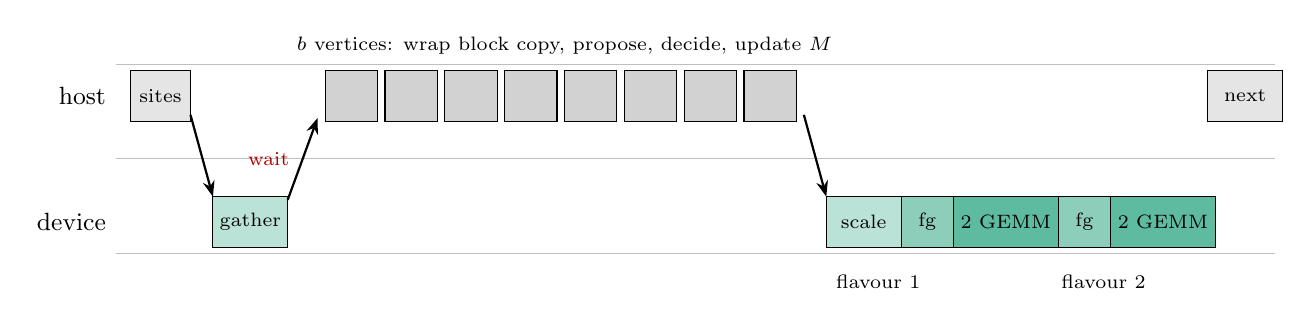
\begin{tikzpicture}[x=0.95cm,y=0.8cm]
\node[anchor=east,font=\small] at (0,2) {host};
\node[anchor=east,font=\small] at (0,0) {device};
\draw[gray!50] (0,2.5)--(15.5,2.5); \draw[gray!50] (0,1)--(15.5,1); \draw[gray!50] (0,-0.5)--(15.5,-0.5);
% block begin
\filldraw[fill=gray!20] (0.2,1.6) rectangle (1.0,2.4); \node[font=\scriptsize] at (0.6,2.0) {sites};
\draw[arr] (1.0,1.7) -- (1.3,0.4);
\filldraw[fill=cA30!30] (1.3,-0.4) rectangle (2.3,0.4); \node[font=\scriptsize] at (1.8,0) {gather};
\draw[arr] (2.3,0.35) -- (2.7,1.65); \node[font=\scriptsize,red!70!black,anchor=east] at (2.45,1.0) {wait};
% host proposals
\foreach \i in {0,...,7} { \filldraw[fill=gray!35] (2.8+\i*0.8,1.6) rectangle (3.5+\i*0.8,2.4); }
\node[font=\scriptsize,align=center] at (6.0,2.8) {$b$ vertices: wrap block copy, propose, decide, update $M$};
\draw[arr] (9.2,1.7) -- (9.5,0.4);
\filldraw[fill=cA30!30] (9.5,-0.4) rectangle (10.5,0.4); \node[font=\scriptsize] at (10.0,0) {scale};
\filldraw[fill=cA30!50] (10.5,-0.4) rectangle (11.2,0.4); \node[font=\scriptsize] at (10.85,0) {fg};
\filldraw[fill=cA30!70] (11.2,-0.4) rectangle (12.6,0.4); \node[font=\scriptsize] at (11.9,0) {2 GEMM};
\filldraw[fill=cA30!50] (12.6,-0.4) rectangle (13.3,0.4); \node[font=\scriptsize] at (12.95,0) {fg};
\filldraw[fill=cA30!70] (13.3,-0.4) rectangle (14.7,0.4); \node[font=\scriptsize] at (14.0,0) {2 GEMM};
\node[font=\scriptsize,align=left,anchor=west] at (9.5,-0.95) {flavour 1 \hspace{1.6cm} flavour 2};
\filldraw[fill=gray!20] (14.6,1.6) rectangle (15.6,2.4); \node[font=\scriptsize] at (15.1,2.0) {next};
\end{tikzpicture}
\caption{One block of the submatrix update in block mode (schematic, not to scale). Host work is grey, device work green; ``fg'' is the flush gather. The only unavoidable wait is the copy of $G_0(B,B)$ to the host at the beginning of the block, because the next gather depends on the previous flush. In the synchronous path every arrow is also a wait.}
\label{fig:block}
\end{figure}

\subsection{Synchronisation points per block}

In the synchronous OpenMP path every \texttt{target} region and every \texttt{target update} returns only when it is complete. In addition \texttt{alf\_la} calls run asynchronously on NVIDIA (cuBLAS returns before the GEMM is done), so two explicit \texttt{la\_sync} calls are needed. The sequence per block (\file{gpu\_lowrank\_mod.F90:1443-1592}):
\begin{enumerate}
\item \texttt{la\_sync} in \texttt{blk\_begin}: the previous flush (asynchronous library calls) must be complete before new uploads overwrite buffers it reads.
\item \texttt{target update to(bsd)}: the block sites.
\item \texttt{k\_blk\_gather}.
\item \texttt{target update from(gbd)}: the host needs $G_0(B,B)$ before it can decide anything. This is the one wait that cannot be removed.
\item \texttt{la\_sync} in \texttt{blk\_end}: ``the previous block's flush (cuBLAS) is asynchronous: it must be done before cbuf / bS\_d are overwritten''.
\item \texttt{target update to(cbuf, bS\_d)}.
\item \texttt{k\_blk\_scale}.
\item Per flavour: \texttt{k\_sub\_flush\_gather} and two \texttt{la\_gemm}. On Intel the dispatched GEMM includes an implicit wait (\file{SYNC.md}).
\item \texttt{target update to(nsigma\_d(vmin:vmax,t))}.
\end{enumerate}
On the A30 a profile of a production layout showed 72\,\% of host time in \texttt{cuStreamSynchronize}, with about 4\,300 blocks and 44\,000 synchronisations per sweep (\file{PP\_GPU.md}, $L=24$, 9 ranks). % PP_GPU.md
In the single-chain profile at $L=32$, 44\,\% of the kernel time was in 32\,338 small ZGEMM flushes of 52~$\mu$s each (\file{TUNING\_DEFECT.md}). % TUNING_DEFECT.md

\subsection{Launch-latency budget of a block}

The Intel team measured where the 167~$\mu$s of wall time of one block go at $L=24$ with V7 (\file{p7/NOTES.md}, line 97): % p7 NOTES
submission of the asynchronous operations 91~$\mu$s, the D$\to$H copy 22~$\mu$s (30 at $L=32$), the hopping 32~$\mu$s, host arithmetic about 20~$\mu$s; the device executes the block in about 65~$\mu$s. The update phase is therefore ``host-submission bound'': the cost of telling the device what to do exceeds the work it does. The per-operation submission costs were 4.4~$\mu$s (gather), 4.5 (flush gather), 4.4 (scale), 9.7 (GEMM) and 9.0 (copy), 0.88~s per sweep in total, 61\,\% of the update phase (\file{p7/NOTES.md}, lines 88-97).

Before the staging buffer setting the D$\to$H of the 32~KB block cost 380~$\mu$s on Intel; with \env{LIBOMPTARGET\_LEVEL\_ZERO\_STAGING\_BUFFER\_SIZE=1048576} it costs 22~$\mu$s, and the update phase went from 4.3 to 1.9~s per sweep (\file{p3/STATUS.md}; \file{ISSUE\_INTEL\_VS\_A30.md}, line 43). % p3 STATUS, ISSUE line 43
``One environment variable gained more than two code phases'' (\file{GPU\_PLAN\_V2.md}, section 2).

\subsection{The asynchronous block path on Intel}
\label{sec:asyncblk}

On NVIDIA, cuBLAS calls are asynchronous by default. On Intel, ifx executes OpenMP \texttt{nowait} target tasks undeferred (97 to 103\,\% of the synchronous cost, \file{p3/STATUS.md}), so OpenMP cannot overlap host and device. The asynchronous block path (\texttt{ALFSH\_ASYNCBLK=1}, \file{gpu\_lowrank\_mod.F90:1328-1347, 1605-1617}; \file{alf\_la\_sycl\_blk.cpp}) bypasses OpenMP for the block operations:
\begin{itemize}
\item It obtains the SYCL queue that the OpenMP runtime uses (\texttt{alfsh\_get\_queue}, through the interop object of \texttt{alf\_la}) and refuses it if it is not \emph{in-order}. ``The queue must be in-order: that, and nothing else, orders the calls'' (\file{alf\_la\_sycl\_blk.cpp:4}).
\item The gather, scale and flush-gather kernels are SYCL ports of the OpenMP kernels with the same expressions and order; the GEMM is oneMKL's \texttt{column\_major::gemm} with the same shapes and scalars; copies are \texttt{queue.memcpy}. All are submitted without waiting. The gathered block lands in host USM memory (memory that the device can write directly).
\item The only wait per block is \texttt{ab\_drain} in \texttt{blk\_begin} after the gather: ``the one unavoidable wait of a block: the host needs G0(B,B)''. \texttt{blk\_end} leaves the block pending; the next \texttt{blk\_begin}, the flush at the end of the slice, or any other device access drains it.
\item The SYCL code is built as a shared library (\file{libalfsb.so}) because SYCL kernels in an object linked by ifx are not found at run time (``No kernel named \ldots'').
\end{itemize}
Results are bitwise identical to the synchronous path. Planted tests: a missing wait gives an ``Unstable matrix'' abort; a missing drain at the end of the slice changes nothing, because the in-order queue orders the OpenMP kernels too (\file{p3/STATUS.md}). Measured effect: $L=24$ 7.05--7.08$\to$6.53--6.59~s per sweep, $L=32$ 23.2$\to$22.0--22.4~s, per card 0.568$\to$0.655--0.688 sweeps/s (\file{ISSUE\_INTEL\_VS\_A30.md}, section 2). % ISSUE section 2

\dis{The release status of \texttt{ALFSH\_ASYNCBLK} differs between notes: \file{RUNTIME\_SWITCHES.md} (line 123) lists it as production, \file{SPEEDUPS.md} (line 21) and \file{NOT\_IMPLEMENTED.md} (line 118) as not yet released. The measured gain is +3\,\% per node in \file{p3/STATUS.md} and +15 to 20\,\% per card in \file{ISSUE\_INTEL\_VS\_A30.md}; the jobs differ.}

\subsection{What remains: the flush}

In production layouts the flush GEMMs are 47\,\% of the kernel time (A30, 9 ranks, \file{PP\_GPU.md}). % PP_GPU.md
They are rank-$k$ updates with $k\approx10$ to 20, bound by memory bandwidth ($N^2$ elements read and written per flush for $2Nk$ new information). The ranked candidate is a two-level submatrix update: one flush per slice of rank about 190 instead of one per block (\file{SPEEDUPS.md}, section 4). It is estimated at weeks of work and not started.

\dis{The header of \file{gpu\_lowrank\_mod.F90} (lines 34, 52-53) calls the module a ``test branch'' where ``numerical agreement is not the goal''. It is the production path, and \file{DELAYED\_SUBMATRIX.md} reports bin-by-bin agreement. The header also describes only the per-proposal gather; block mode is documented only at line 1253.}

\section{Observables}
\label{sec:obs}

Measurements in ALF are model code: each Hamiltonian's \texttt{Obser} and \texttt{ObserT} read $G$ and accumulate into observable objects. A general port would need a device version of every model's measurement routine. The port does this for the predefined Hubbard model only (\file{Prog/gpu\_obs\_mod.F90}, 785 lines; time-displaced part in \file{gpu\_tau\_mod.F90}). For other models the GPU path downloads $G$ and the host measures.

\subsection{Hook-up and conditions}

\texttt{gpu\_obs\_setup} is called at the end of \texttt{Alloc\_obs} of \file{Hamiltonian\_Hubbard\_smod.F90} (lines 788-789) with the lattice, the hopping matrix and the parameters. \texttt{Obser} begins with
\begin{lstlisting}
if (gpu_obs_active()) then; call gpu_obs_measure(...); return
\end{lstlisting}
(lines 831-837). \texttt{gpu\_obs\_active} requires: setup done, the model checks passed, \texttt{ALF\_GPU\_NOOBS} not set, the GPU path and the device update active. The model checks (\file{gpu\_obs\_mod.F90:92-184}) are: no projector; $\NFL\in\{1,2\}$; the expected number of equal-time observables (5 for $\NFL=2$, else 3); $N=N_{\rm cell}N_{\rm orb}$; the displacement table \texttt{Latt\%imj} a bijection per site; with the pinning field ($h_0\ne0$) $\NFL=2$ and two local observables. If a check fails the run measures on the host; this is a silent fallback, not a refusal.

In \file{main.F90} (lines 1033, 1109) the download of $G$ before the measurement is skipped when the device measures, and \texttt{Hop\_mod\_Symm} is skipped when the device applies \texttt{Symm}.

\subsection{What is measured}

Let $\bar G_{ij}=\delta_{ij}-G_{ji}$ (\texttt{GRC} in ALF) and $w=Z_PZ_S$ the phase and sign weight, passed to the kernels as two reals.

\paragraph{Scalars} (\file{gpu\_obs\_mod.F90:300-341}):
\begin{align}
Z_{\rm kin} &= N_{\rm SUN}\sum_{k} h_k\,\bar G_{i_k j_k f_k}, \\
Z_{\rm pot} &= \sum_{I,o}U_o\,(1-G_{ii,\uparrow})(1-G_{ii,\downarrow}),\qquad
Z_\rho = N_{\rm SUN}\sum_{i,f}(1-G_{ii,f}),
\end{align}
and the total energy $Z_{\rm kin}+Z_{\rm pot}$. The kinetic energy is a sparse linear functional of $G$, built once on the host as a list of $(h_k,i_k,j_k,f_k)$ from the hopping matrix (a copy of \texttt{Predefined\_Hoppings\_Compute\_Kin}, without the pinning term).

\paragraph{Correlation functions} (\file{gpu\_obs\_mod.F90:404-525}). For $\NFL=2$ the kinds are Green, SpinZ, SpinXY, SpinT and Den; for $\NFL=1$ Green, SpinZ (SU($N$)) and Den. For each pair of sites $(i,j)$ with displacement $d=i-j$ and orbitals $(o,o')$ the kernel accumulates into $\texttt{acc}(d,o,o',\text{kind})$ the expressions of \texttt{Predefined\_Obs\_eq\_*\_measure}, for example
\begin{align}
\text{Green:}&\quad N_{\rm SUN}\sum_f\bar G_{ij,f},\qquad
\text{SpinSUN:}\quad N_{\rm SUN}\,\bar G_{ij}G_{ij},\\
\text{Den:}&\quad z_iz_j + N_{\rm SUN}\sum_f\bar G_{ij,f}G_{ij,f},\qquad z_i=N_{\rm SUN}\sum_f (1-G_{ii,f}),
\end{align}
and for $N_{\rm SUN}=1$ the $zz$, $xy$ and $T=(2xy+zz)/3$ spin correlations in one kernel.

\paragraph{The \texttt{acc0} terms.} ALF stores with each correlation function the one-site expectation per orbital, \texttt{Obs\_Latt0}, which the analysis subtracts to obtain connected correlations. The device keeps it in \texttt{acc0}$(N_{\rm orb},n_{\rm obs})$: for Den, $N_{\rm SUN}\sum_I\sum_f(1-G_{ii,f})\,w$; for SpinZ, $\sum_I[(1-G_{ii,2})-(1-G_{ii,1})]\,w$, and the same divided by $\sqrt3$ for SpinT; Green and SpinXY have none (\file{gpu\_obs\_mod.F90:471-523}; host: \file{Predefined\_Obs\_mod.F90:190-191, 322}). The \texttt{acc0} sum used to run serially on one GPU thread, 760~$\mu$s per call and 7\,\% of the kernel time at $L=24$; it is now one team per orbital with a parallel reduction (comment at lines 471-472). On NVIDIA this gave no measurable gain (88.9~s against 88.9~s, \file{PP\_GPU.md}); on Intel it gave 4.92--4.98$\to$4.42--4.48~s per sweep at $L=24$ (\file{SPEEDUPS.md}, section 1). % PP_GPU.md lines 41-42; SPEEDUPS.md sec 1
Results changed by at most $3.3\times10^{-16}$ (\file{CONSOLIDATION.md}).

\paragraph{Point-defect observables} (\file{gpu\_obs\_mod.F90:361-402}). Per site and orbital $d=(G_{ii,2}-G_{ii,1})\,w$ is accumulated into \texttt{lacc1} (\texttt{SpinZ\_local}) and into \texttt{lacc2}$(\cdot,\tau,\cdot)$ (\texttt{SpinZ\_localtau}) with index $\tau+1-T_{\rm htrot}$, weight 2 at the end points; the counter is incremented at $\tau=\Lt/2$. This mirrors \file{Hamiltonian\_Hubbard\_smod.F90:901-922}.

\subsection{How the reductions are organised}

A reduction (a sum of many numbers into one) is the operation where a GPU and a CPU differ most. A naive parallel sum with \emph{atomic} additions is non-deterministic: the order of additions, and so the rounding, changes from run to run. The port avoids atomics everywhere:
\begin{itemize}
\item \textbf{Scalars} (OpenMP path): one \texttt{target teams distribute parallel do reduction(+:...)} kernel per scalar.
\item \textbf{Correlations} (OpenMP path): one \emph{team} (a group of threads that can synchronise) per output element $m=(d,o,o')$, via \texttt{target teams distribute} over $N_{\rm cell}N_{\rm orb}^2$ elements; inside the team a \texttt{parallel do reduction(+:...)} over the $N$ sites; then one thread adds the result into \texttt{acc}. Each output element belongs to exactly one team, so there are no conflicts.
\item \textbf{HIP path} (AMD): \texttt{hk\_scalars} is one block of 128 threads with strided partial sums and a tree reduction in shared memory; six doubles come back in one copy. \texttt{hk\_corr} launches one block per output element plus $N_{\rm orb}$ blocks for the \texttt{acc0} sums, each with a tree reduction (\file{alf\_hip\_kernels.hip.cpp:157-262}).
\end{itemize}
The work per measurement is $O(N^2)$ per kind (all pairs $i,j$), the same as on the CPU.

\paragraph{Transfers.} $G$ is read from \texttt{G\_d} directly. The reduced scalars come back per measurement. The accumulators \texttt{acc}, \texttt{acc0}, \texttt{lacc1}, \texttt{lacc2}, \texttt{tacc}, \texttt{tacc0} are downloaded once per bin by \texttt{gpu\_obs\_flush} (called from \file{main.F90:1337} before \texttt{Pr\_obs}), zeroed and uploaded. Counters, the scalar accumulation into \texttt{Obs\_scal}, normalisation, binning, the MPI reduction and I/O stay on the host.

\paragraph{\texttt{Symm}.} With the symmetric Trotter decomposition, $G$ is saved, transformed in place by $A(A_{td}GB_{td})B$ (two to four GEMMs) and restored after the measurement (\file{gpu\_obs\_mod.F90:268-284, 354-358}).

\paragraph{Skipping.} \texttt{ALF\_GPU\_OBS\_SKIP} takes a list of kinds 1 to 4 (Green, SpinSUN, Den, SpinMz) that are not measured and stay zero. Skipping Green and Den saved 7\,\% under MPS (\file{PP\_GPU.md}). % PP_GPU.md
It is meant for production runs that do not need those observables.

\dis{The header of \file{gpu\_obs\_mod.F90} says the supported case needs ``$|h_0|<$ Eps\_small; no Symm'' (line 12), that the sum over $I$ is ``a sequential loop per output element'' (line 20), and that the scalars are ``one D$\to$H of three complex numbers per slice'' (line 16). The code supports the defect and \texttt{Symm}, sums with a parallel reduction inside each team, and on the OpenMP path returns three separate reduction results.}

\subsection{The time-displaced pass}

With \texttt{Ltau=1}, \file{tau\_m\_mod.F90:82-83} calls \texttt{gpu\_tau\_pass} when the device $\tau$ pass is on. Conditions (\file{gpu\_tau\_mod.F90:234-283}): device stabilisation on, \texttt{Ltau=1}, no projector, no weight reconstruction. Setup reserves all library work space and runs one $2N$ QR so that nothing is allocated during the sweep.

\paragraph{Algorithm.} \texttt{tau\_begin} sets on the device $G(0,0)=G(\tau,0)=G(\tau,\tau)=G$ and $G(0,\tau)=-(1-G)$, keeps a copy of $G$ as precision reference, and resets the right $UDV$ slot. For each slice (\texttt{tau\_slice}, lines 448-467):
\begin{align}
G(\tau{+}1,0) &= B_{\tau+1}\,G(\tau,0) \qquad(\texttt{gpu\_mmthr}, \texttt{gpu\_Vslice\_R}),\\
G(0,\tau{+}1) &= G(0,\tau)\,B_{\tau+1}^{-1}\qquad(\texttt{gpu\_mmthl\_m1}, \texttt{gpu\_Vslice\_L}),\\
G(\tau{+}1,\tau{+}1) &= B_{\tau+1}\,G(\tau,\tau)\,B_{\tau+1}^{-1}.
\end{align}
At every stabilisation point the right state is propagated and decomposed on the device, the left state is read in place from the stack slot (no copy), and \texttt{dev\_cgr22} recomputes the four Green functions from the $2N\times2N$ block matrix of \texttt{CGR2\_2}. The steps of \texttt{dev\_cgr22} (lines 574-678): the branch $D_1(1)>D_2(1)$ from two scalars D$\to$H; $V_1^{-1}$ by LU (\texttt{getrf} plus \texttt{getrs} on the identity, where the CPU uses \texttt{ZGETRI}); the scale splitting; the $2N\times2N$ matrix; QR with pre-pivoting (or host \texttt{ZGEQP3} with \texttt{STABLOG}); triangular solve and scaling; $QX$ through an explicit $Q$ with a Newton--Schulz step and a GEMM. With cuSOLVER's \texttt{ZUNMQR} applied directly the precision of the $\tau$ pass was 17\,\% worse on average and up to 2 times worse at the maximum than on the CPU; with the explicit $Q$ and the step it was $6.75\times10^{-12}$ against $7.36\times10^{-12}$ on the CPU (header lines 56-59). % gpu_tau_mod.F90 header
The four precision checks of \texttt{Control\_Precision\_tau} run as device reductions, four numbers each.

\paragraph{Observables.} If \texttt{gpu\_obs\_tau\_active()}, every slice calls \texttt{gpu\_obs\_tau\_measure} with the four device matrices. The kernel \texttt{tcorr} (\file{gpu\_obs\_mod.F90:648-783}) accumulates the same kinds as the equal-time measurement, resolved in $\tau$, into \texttt{tacc}$(N,N_\tau,N_{\rm orb},N_{\rm orb},n_{\rm obs})$, e.g.\ SpinSUN $-N_{\rm SUN}\,G(0,\tau)_{ji}\,G(\tau,0)_{ij}$. This removes a D$\to$H of $3N^2$ complex numbers per slice and flavour. The \texttt{tacc0} loops are still serial over $N$ per orbital; under HIP \texttt{tcorr} stays an OpenMP kernel with a serial inner sum, unlike the equal-time HIP kernels.

\paragraph{What is refused.} The device $\tau$ pass is off with \texttt{Ltau}$\ne1$, the projector, weight reconstruction or without device stabilisation; then the CPU pass runs on downloaded data. The device $\tau$ observables are off with the point defect; in practice this case cannot occur because \texttt{Ham\_Set} sets $h_0=0$ when \texttt{Ltau=1} (\file{Hamiltonian\_Hubbard\_smod.F90:247-259}). Debug and fault variables of the $\tau$ pass are refused in production runs.

\dis{The header of \file{gpu\_tau\_mod.F90} (line 46) and the info line printed at setup (line 275) still say ``observables on the host, interim''; since ticket 208-3 they are measured on the device. \file{TUNING\_DEFECT.md} also says ``host ObserT''. The device $\tau$ observables apply only the static \texttt{Symm} matrices, while the host path calls \texttt{Hop\_mod\_Symm} with the slice arguments; this matters only with time-dependent hopping, which is switched off for \texttt{Ltau=1}. \texttt{gpu\_obs\_tau\_active} does not test \texttt{gpu\_upd\_enabled}, while \texttt{gpu\_obs\_active} does: with \texttt{ALF\_GPU\_NOUPDATE=1} the equal-time observables move to the host and the $\tau$ observables stay on the device. \file{main.F90:1301} downloads $G$ before every $\tau$ pass although the device pass does not need it.}

\paragraph{Evidence.} \texttt{Ltau=1} has been run on NVIDIA; it has not been run on the Max~1550 or the MI210 according to \file{FEATURES.md} (lines 61, 97).

\section{MPI, parallel parameters and sharing a GPU}
\label{sec:mpi}

\subsection{What MPI does in a GPU run}

ALF's MPI parallelism is over independent Markov chains: each rank runs its own sweep, and only the observables are reduced at the end of a bin. The GPU port keeps this. Every rank builds its own device mirror and its own device $G$ and stacks, draws its own random numbers on the host, and talks to the other ranks only through the host-side observable reduction (\file{gpu\_state\_mod.F90:516-519}). No GPU-aware MPI is needed.

\paragraph{Rank-to-device binding.} The code sets the OpenMP default device to
\begin{lstlisting}
call omp_set_default_device(mod(env_rank, omp_get_num_devices()))
\end{lstlisting}
(\file{gpu\_state\_mod.F90:550-552}), where \texttt{env\_rank} is the rank in \texttt{MPI\_COMM\_WORLD}. In practice the job scripts restrict each rank to one device before the program starts, so the rule always yields device 0:
\begin{itemize}
\item NVIDIA (Helma): a wrapper sets \env{CUDA\_VISIBLE\_DEVICES} $=r/\text{ranks per GPU}$ from the Open MPI rank $r$, and with MPS the pipe and log directory of that GPU's MPS daemon (\file{docs/gpu/scripts/helma/rank\_wrap.sh}). The device used by the OpenACC stream query (Section~\ref{sec:design}) must be the OpenMP default device, which this binding guarantees.
\item Intel (SuperMUC-NG Phase 2): \env{ZE\_FLAT\_DEVICE\_HIERARCHY=FLAT} exposes the 8 tiles of a node's four Max~1550 cards as 8 devices, so rank $r$ uses tile $r\bmod8$; with fewer ranks \env{ZE\_AFFINITY\_MASK} binds them (\file{intel\_pvc\_supermuc\_ng2.md:26-27}).
\item AMD: no MPI run is documented (\file{FEATURES.md}, line 47).
\end{itemize}

\dis{The binding uses the global rank, not the node-local rank. On several nodes the mapping is right only if the ranks are placed in blocks and the number of ranks per node is a multiple of the number of devices. This is not documented; the job scripts avoid the issue by setting the visible devices per rank.}

\paragraph{Correctness.} One MPI rank reproduces the non-MPI run to $10^{-12}$ (energy $7\times10^{-12}$, \texttt{SpinZ\_localtau} $1.4\times10^{-12}$, \texttt{SpinZ\_local} $7\times10^{-15}$), and acceptance (0.3375) and precision ($10^{-14}$) do not depend on the number of ranks (\file{MPI\_GPU.md}). % MPI_GPU.md

\subsection{Parallel parameters and tempering}

With \texttt{TEMPERING} and \texttt{PARALLEL\_PARAMS} ALF runs groups of ranks with different parameter sets. Real parallel tempering (exchange of configurations between parameter sets) is refused on the GPU path. Parameter-parallel runs without exchange are allowed: the groups are independent, and \file{main.F90} skips \texttt{Exchange\_Step} (\file{PP\_GPU.md}). Build: \texttt{configure.sh PGI PP GPU=nvidia HDF5} with \texttt{PP = -DMPI -DTEMPERING -DPARALLEL\_PARAMS}.

\subsection{Several ranks on one GPU}

One chain does not fill a GPU: on the A30 one chain kept the GPU busy 58\,\% of the time, two chains 82\,\% (\file{MPI\_GPU.md}, \texttt{nvidia-smi dmon}); on the H100 at $L=32$ one chain used 55\,\% of the streaming multiprocessors (\file{helma\_h100.md}, section 4.2). % MPI_GPU.md; helma_h100.md 4.2
The reason is the structure of the work: most kernels are small (block gathers, rank-$k$ flushes, single-vertex wraps) and the host spends time between them. Running several chains per GPU fills the gaps. How well this works depends on how the GPU shares itself between processes.

\paragraph{NVIDIA: MPS.} Without help, processes on one NVIDIA GPU are \emph{time-sliced}: the GPU switches between their contexts, and kernels of different processes never run at the same time. The \emph{Multi-Process Service} (MPS) merges the processes into one context, so their kernels run concurrently. \env{CUDA\_MPS\_ACTIVE\_THREAD\_PERCENTAGE} limits the share of the GPU each client can use. Measured:
\begin{itemize}
\item Without MPS, two processes on the A30 ran 13 to 15 times slower each (\file{CLAUDE.md}); on the H100 two ranks were 6.5 times slower per chain at $L=24$ (29.5 against 4.54~s per sweep) and 2.6 times at $L=32$; four or eight ranks at $L=32$ did not finish six sweeps in 420~s (\file{helma\_h100.md}, section 4). % helma_h100.md
\item With MPS the throughput rises with the number of ranks. Table~\ref{tab:mps} gives the A30 at $L=16$.
\item A 25\,\% thread share was 12\,\% faster than no limit with 9 ranks at $L=24$ (86.9 against 98.3~s for 10 sweeps, \file{PP\_GPU.md}); 25\,\% and 50\,\% agree within 2\,\% on the H100. % PP_GPU.md; helma_h100.md
\end{itemize}

\begin{table}[h]
\centering\small
\caption{A30, $L=16$, submatrix $\Nd=32$, 30 sweeps, with MPS (\file{MPI\_GPU.md}).}
\label{tab:mps}
\begin{tabular}{@{}rlrrr@{}}
\toprule
Ranks & MPS share & Time per chain (s) & vs 1 rank & Sweeps/s per GPU \\
\midrule
1 & 100\,\% & 38.8 & -- & 0.73 \\ % MPI_GPU.md
2 & 50\,\% & 45.3 & +17\,\% & 1.25 \\
4 & 25\,\% & 54.6 & +41\,\% & 2.09 \\
8 & 13\,\% & 81.4 & +110\,\% & 2.83 \\
16 & default & 145.6 & +275\,\% & 3.18 \\
16 & 25\,\% & -- & -- & 4.68 \\
\bottomrule
\end{tabular}
\end{table}

On the H100 at $L=24$ one rank gives 0.285 sweeps per second, eight ranks with MPS at 25\,\% give 1.176, 4.1 times more, while each chain becomes 1.9 times slower (6.80 against 3.51~s per sweep). At $L=32$: 0.102 with one rank, 0.232 with eight and 0.250 with sixteen (\file{helma\_h100.md}, sections 4.1-4.2). % helma_h100.md
MPS does not change the results: two MPS clients produced output bit-identical to a solo run (\file{CLAUDE.md}).

\paragraph{Intel: CCS.} The Max~1550 has no MPS. Ranks sharing a tile are time-sliced by default. The compute command streamer setting \env{ZEX\_NUMBER\_OF\_CCS=0:4,\ldots,7:4} splits each tile into four hardware queues, so four processes can run concurrently on one tile. With the V7 switches at $L=24$ the throughput per card is 0.365, 0.458, 0.879 and 0.261 sweeps per second for 1, 2, 4 and 8 walkers per tile (\file{ISSUE\_INTEL\_VS\_A30.md}, section 7). % ISSUE section 7
Four walkers per tile (32 ranks per node) is the optimum.

\dis{\file{intel\_pvc\_supermuc\_ng2.md} (line 45, 2026-11-10) reports that CCS 4 gave ``no gain'' and recommends one rank per tile (line 47); \file{RUNTIME\_SWITCHES.md} (line 173) and the later session notes report CCS 4 with 32 ranks per node as the throughput optimum. The later measurement is the one used in production.}

\paragraph{AMD.} Four concurrent processes on the MI210 without any sharing service gave 1.95 times the throughput of one (\file{SPEEDUPS.md}, section 3); compute-unit masking (\env{HSA\_CU\_MASK}) gave nothing. % SPEEDUPS.md

\subsection{The production layout}

The production layout is a measured per-platform setting (\file{GPU\_PLAN\_V2.md}, section 2): on the H100, eight ranks per GPU with MPS at 25\,\%, $\Nd=64$ at $L=32$ (\file{helma\_h100.md}, section 7); on the Max~1550, four ranks per tile with CCS 4; on the A30 the owner decided on one rank per GPU (2026-11-08, \file{MPI\_GPU.md}). The choice of $\Nd$ interacts with the layout: with eight ranks on the H100 at $L=32$, $\Nd=32$ gave 66.5~s per sweep per chain and $\Nd=64$ gave 34.5~s (\file{helma\_h100.md}, section 4.2). % helma_h100.md

\section{The three backends in detail}
\label{sec:backends}

The physics code is the same for all three vendors. What differs is the compiler, the library behind \texttt{alf\_la}, and, on Intel and AMD, a layer of native kernels. Table~\ref{tab:backends} gives the overview; the subsections give the problems met and how they were solved.

\begin{table}[h]
\centering\small
\caption{Backends as built and run.}
\label{tab:backends}
\begin{tabularx}{\textwidth}{@{}lXXX@{}}
\toprule
 & NVIDIA & Intel & AMD \\
\midrule
Macro & \texttt{ALF\_LA\_CUDA} & \texttt{ALF\_LA\_ONEMKL} & \texttt{ALF\_LA\_HIP} \\
Hardware run & A30 (nividia), H100 (Helma) & Max 1550 (SuperMUC-NG Phase 2); Arc B580 for tests & MI210 \\
Compiler & nvfortran 26.9 (A30), nvhpc 25.7 (H100) & ifx 2025.1 (production), 2025.3 & gfortran 14 with amdgcn offload \\
Offload flags & \texttt{-mp=gpu -gpu=cc80|cc90} & \texttt{-fiopenmp -fopenmp-targets=spir64} & \texttt{-foffload=amdgcn-amdhsa} \\
BLAS/LAPACK & cuBLAS, cuSOLVER & oneMKL (OpenMP dispatch + SYCL shim) & hipBLAS, hipSOLVER, own HIP QR \\
Native kernels & none & SYCL: \file{libalfsb.so}, \file{libalfdevqr.so} & HIP: \file{alf\_hip\_kernels}, \file{alf\_hip\_qr} \\
Stream handling & \texttt{acc\_async\_sync} stream & interop in-order SYCL queue & default stream, deferred sync \\
\bottomrule
\end{tabularx}
\end{table}

\subsection{NVIDIA}

\paragraph{Toolchain.} On the development machine nividia (A30, 24~GB) nvfortran 26.9; on Helma (4$\times$H100 per node, 95.8~GB) nvhpc 25.7 with Open MPI 5.0.8 and \texttt{-gpu=cc90,cuda12.9} (\file{helma\_h100.md}, section 2). cuBLAS and cuSOLVER are linked with \texttt{-cudalib=cublas,cusolver}.

\paragraph{Problems and solutions.}
\begin{itemize}
\item \textbf{Complex scalar arguments in target regions.} nvfortran dropped the imaginary part of a complex scalar \texttt{intent(in)} dummy inside a target region; $G$ was wrong by $10^{-3}$ to 1. All complex scalars passed to kernels are now two reals (\file{DISCREPANCIES.md}; \file{gpu\_update\_mod.F90:316-317}, \file{gpu\_obs\_mod.F90:25}).
\item \textbf{Stream ordering.} A created CUDA stream did not order cuBLAS calls against OpenMP target regions. The fix is the stream \texttt{acc\_get\_cuda\_stream(acc\_async\_sync)}; the unit test \texttt{t\_order} detects a wrong choice (\file{alf\_la\_mod.F90:48-61}). nvfortran does not implement \texttt{!\$omp interop} (warning W-0287), hence the detour through the OpenACC runtime.
\item \textbf{Alignment.} cuBLAS crashed when complex \texttt{alpha}/\texttt{beta} were only 8-byte aligned; they are now held in a 16-byte aligned module array (ticket 101).
\item \textbf{Miscompilation of \texttt{blk\_end}.} At \texttt{-O2}/\texttt{-O3} nvfortran 26.9 produced a wrong $G$ after the first stabilisation; the routine is pinned to \texttt{-O1} (\texttt{!pgi\$r opt=1}).
\item \textbf{Stale \texttt{target update from}.} At \texttt{-fast} a \texttt{target update from} of a module allocatable returned stale data, and a fourth $N\times N\times\NFL$ array in \file{gpu\_state\_mod} crashed the compiler (heap corruption in \texttt{fort1}) when compiling \file{gpu\_stab\_mod}. Workaround: helper routines \texttt{upd\_*} and moving \texttt{G00\_d} to \file{gpu\_tau\_mod} (\file{gpu\_tau\_mod.F90:103, 141-144, 515}).
\item \textbf{\texttt{present} map modifier} is rejected by nvfortran 26.9; \texttt{map(alloc:)} is used.
\item \textbf{nvhpc 24.11} on Helma needs CUDA 12.6 (CUDA 11.8 lacks \texttt{cusolverDnSetDeterministicMode}) and then aborts at $L=8$ with ``la\_qrpp: NaN or Inf in the matrix''; 25.7 works (\file{helma\_h100.md}, section 2; \file{configure.sh:502-510}).
\item \textbf{Orthogonality of cuSOLVER's $Q$} needed the Newton--Schulz step (Section~\ref{sec:stab}).
\item \textbf{Processes without MPS} are time-sliced and very slow (Section~\ref{sec:mpi}).
\end{itemize}

\subsection{Intel}
\label{sec:intel}

\paragraph{Toolchain.} ifx with OpenMP offload to SPIR-V (\texttt{-fopenmp-targets=spir64}), oneMKL with its OpenMP offload interface for BLAS, and a C++/SYCL shim for LAPACK. On SuperMUC-NG Phase 2 only oneAPI 2025.1 works in production: 2025.3 compiles, but the OpenMP-to-SYCL interop crashes with the Level Zero V2 adapter (\file{intel\_pvc\_supermuc\_ng2.md}; \file{GPU\_PLAN\_V2.md}, section 2).

\dis{\file{CONSOLIDATION.md} records the verification of 2026-11-13 on the Max~1550 with ifx 2025.3, while the platform page says 2025.3 crashes at run time. \file{PLAN.md} and \file{DECISIONS.md} item 13 pin ifx 2026.2 for the test workstation. \file{NOT\_IMPLEMENTED.md} (line 95) lists the question as open.}

\paragraph{How BLAS and LAPACK reach the device.} BLAS calls are written as ordinary Fortran calls preceded by \texttt{!\$omp dispatch}; with \texttt{use onemkl\_blas\_omp\_offload\_lp64} ifx replaces the call by oneMKL's device variant when the arguments are mapped. LAPACK through \texttt{dispatch} would run partly on the host, so the factorisations go through a SYCL shim (\file{alf\_la\_sycl\_shim.cpp}): the Fortran side creates an OpenMP interop object of type SYCL, extracts the \texttt{sycl::queue*}, and passes it with device addresses to C++ routines that call \texttt{oneapi::mkl::lapack::*} on that queue and wait. A probe checks that the OpenMP default device is the queue's device.

\paragraph{Problems and solutions.}
\begin{itemize}
\item \textbf{Missing interop symbols.} ifx up to 2025.3 lacks \texttt{omp\_get\_interop\_int/ptr} and the \texttt{omp\_ipr\_*} constants in \texttt{omp\_lib}; they are declared with \texttt{bind(C)} and the OpenMP 5.1 values in \file{alf\_la\_mod.F90:142-145, 175-189}.
\item \textbf{SYCL kernels in ifx-linked objects} are not found at run time; the SYCL code is built into shared libraries (\file{libalfsb.so}, \file{libalfdevqr.so}).
\item \textbf{Unmapped arrays.} An unmapped array passed to the queue once hard-reset the Arc workstation; \texttt{need\_present} checks the first and last element with \texttt{omp\_target\_is\_present} before every queued call (\file{alf\_la\_mod.F90:290-306}).
\item \textbf{Descriptor copies.} ifx copies the descriptors of module allocatables referenced in target regions at every launch; explicit-shape dummies cut the first-private arrays from 168\,800 to 28\,544 and launches from about 75\,000 to 49\,530 per sweep, worth 0.4 to 1.2~s at $L=24$ (\file{report/sections/s6\_performance.tex}, from \file{ISSUE\_INTEL\_VS\_A30.md}). % ISSUE_INTEL_VS_A30.md
\item \textbf{Staging buffer.} The default Level Zero staging buffer made the 32~KB block copy cost 380~$\mu$s; a 1~MB buffer brings it to 22~$\mu$s (Section~\ref{sec:updates}).
\item \textbf{No asynchrony through OpenMP.} ifx runs \texttt{nowait} target tasks undeferred; asynchrony through SYCL on the interop queue (Section~\ref{sec:asyncblk}).
\item \textbf{Hybrid oneMKL QR and slow \texttt{getrf}.} Own device QR (Section~\ref{sec:ownqr}) and the LU-free phase (Section~\ref{sec:stab}). \texttt{getrf} uses 64-bit pivots; a target loop converts them to the 32-bit pivots of the interface.
\item \textbf{Ahead-of-time compilation.} A wrapper rewrites the target flag to \texttt{spir64\_gen -device pvc}; start-up falls from about 65~s (just-in-time compilation of the kernels) to 14~s (\file{intel\_pvc\_supermuc\_ng2.md}). % intel_pvc_supermuc_ng2.md
\item \textbf{Faulty hardware.} All seven ``Unstable matrix'' aborts of a production series came from tile 1 of one node; the node is excluded and the precision threshold lowered (\file{DECISIONS.md}, item 46).
\end{itemize}

\paragraph{The optimisation steps, measured.} Each step is a run-time switch of one binary, measured by alternating runs in one job (\file{ISSUE\_INTEL\_VS\_A30.md}, section 2). Table~\ref{tab:intelsteps}.

\begin{table}[h]
\centering\small
\caption{Max~1550, one chain per tile, seconds per sweep; per card with 4 ranks per tile and CCS 4. Mid-points of the measured ranges (\file{ISSUE\_INTEL\_VS\_A30.md}, section 2; \file{SPEEDUPS.md}).}
\label{tab:intelsteps}
\begin{tabular}{@{}llrrr@{}}
\toprule
Step & Switch & $L=24$ & $L=32$ & sweeps/s per card \\
\midrule
V0 & none & 10.6 & 31.0 & 0.549 \\ % ISSUE sec 2
V1 & staging buffer 1~MB & 7.07 & 23.2 & 0.568 \\
V2 & + \texttt{ALFSH\_ASYNCBLK=1} & 6.56 & 22.2 & 0.67 \\
V4 & + \texttt{ALFSH\_DEVQR=1} & 6.15 & 19.4 & 0.76 \\
V7 & + \texttt{DEVQR=2}, \texttt{DEVUNMQR=1} & 4.96 & 16.4 & 0.86 \\
& + parallel \texttt{acc0} & 4.42--4.48 & & \\ % SPEEDUPS.md sec 1
& + LU-free phase & 4.04 & & \\ % SPEEDUPS.md sec 2
\bottomrule
\end{tabular}
\end{table}

\subsection{AMD}
\label{sec:amd}

\paragraph{Toolchain.} gfortran 14 with offload to \texttt{amdgcn-amdhsa} (\texttt{-march=gfx90a}); hipBLAS and hipSOLVER through a small C++ shim compiled with g++; own kernels compiled with \texttt{hipcc}. \texttt{-ffast-math} is removed for \texttt{GPU=amd}: the $L=6$ test became unstable with it (\file{configure.sh:624-630}).

\paragraph{The launch cost of the GCC runtime.} The OpenMP runtime of GCC (libgomp) launches kernels on AMD GPUs through its GCN plugin. An empty target region cost 253~$\mu$s, a target region with a parallel loop about 150~$\mu$s, against about 15~$\mu$s for a HIP launch plus synchronisation (\file{amd\_mi210/README.md}; \file{alf\_hip\_kernels.hip.cpp:2}). % amd README
With tens of thousands of launches per sweep this alone made the port useless. Three measures:
\begin{enumerate}
\item \textbf{A patched plugin} (\file{plugin-gcn-pool-prof.patch} for GCC 14.2.0): it pools the kernel argument block and the completion signal and small device allocations. An empty target region falls from 253 to 37~$\mu$s; about 3 times faster on the real run. \env{GCN\_NUM\_THREADS=4} instead of 16 was best.
\item \textbf{HIP kernels} for all small operations (\file{alf\_hip\_kernels.hip.cpp}, 621 lines, called through \file{alf\_hipk\_mod.F90}): block gather, scale, fused block end, flush gather, the observable kernels, the stabilisation helpers (row division, Newton--Schulz, phase, precision check, permutations), the vertex slice multiplication, the column norms and permutations of \texttt{la\_qrpp}. Under \texttt{\#if defined(ALF\_LA\_HIP)} they replace OpenMP kernels in \file{Prog/gpu\_*.F90}.
\item \textbf{Deferred synchronisation} (\file{plugin-gcn-presync-hook.patch}, \env{ALF\_HIP\_ASYNC}): normally every HIP call ends with \texttt{hipDeviceSynchronize}. With the patch the plugin calls a function registered by ALF before it launches an OpenMP kernel or copies data; only then are pending HIP operations synchronised. Output is bit-identical.
\end{enumerate}
Together with the own QR (Section~\ref{sec:ownqr}): $L=16$, two sweeps, 66~s with stock GCC, 21~s with the plugin, threads and observable kernels, 6~s with the HIP kernels; $L=24$ 95$\to$19~s (\file{amd\_mi210/README.md}). Steady state: 4.41~s per sweep at $L=24$ and 17.5~s at $L=32$. % amd README

\dis{The comments in \file{alf\_la\_hip\_mod.F90} (lines 5-6) and \file{alf\_la\_hip\_shim.cpp} (lines 2-4) say every call ends with \texttt{hipDeviceSynchronize}; with the patched plugin this is no longer true for BLAS and own kernels. The \texttt{ALF\_LA\_TEST\_*} hooks are declared but not armed in the HIP backend.}

\subsection{What would a fourth backend need}

From the three experiences: an implementation of the \texttt{om\_*} (or CUDA-style) routines of \texttt{alf\_la}; a check that library calls and OpenMP kernels are ordered (the test \texttt{t\_order}); a measurement of the launch cost of OpenMP target regions, and if it exceeds about 20~$\mu$s, native kernels for the small operations; a measurement of the vendor QR, and an own QR if it is slow or hybrid. An Apple GPU was evaluated and rejected: Metal has no double precision; emulated double-double ZGEMM reached 290~GFlop/s against 460 to 520~GFlop/s of the CPU's matrix unit, and inside ALF at $L=24$ it saved 0.6~s of 115~s while worsening the precision of $G$ from $1.6\times10^{-12}$ to $6.7\times10^{-11}$ (\file{APPLE\_GPU\_FEASIBILITY.md}). % APPLE_GPU_FEASIBILITY.md

\section{Verification}
\label{sec:verif}

A Monte Carlo code is hard to test: the output is noisy, the trajectory is chaotic, and the random number stream differs between compilers. The port went through two verification regimes. The first relied on statistical acceptance gates and was abandoned; the second relies on deterministic comparisons and is the standard now. Both are described, because the contrast is the main lesson.

\subsection{The method that worked}

\paragraph{1. Same-compiler CPU reference at fixed seed.} The host draws the same random numbers in the same order as the CPU code, and makes the same accept/reject decisions from the same ratios. If the device computes $G$ to rounding accuracy, a GPU build and a \texttt{GPU=none} build of the same compiler with the same parameters and seed follow the same Markov chain. A wrong decision would occur only if a ratio lies within rounding of a random number, which over a short run does not happen. The observables then agree to rounding: about $10^{-13}$ with \texttt{Mz=.F.} and about $10^{-10}$ with \texttt{Mz=.T.}, where the coupling is complex and the trajectory more sensitive (\file{README.md}, ``How correctness is checked''). % README.md
The comparison script is \file{scripts/defect/run\_cmp.py}. The same compiler matters: random streams differ between gfortran, nvfortran, ifx, so trajectories cannot be compared across compilers.

The rule for large lattices was refined on 2026-11-11 (\file{DECISIONS.md}, item 43): for $L\ge16$ on the Max~1550, $10^{-13}$ is not reachable in the imaginary parts of the scalar observables because of the summation order. The rule now is: configurations (\texttt{confout}) bitwise identical; real parts within 10 times the spread between two CPU runs; imaginary parts of the scalars reported only. The bitwise identity of the configurations is the strongest test: it means every one of the millions of decisions was the same.

\paragraph{2. Deterministic kernel tests.} Each device routine has a self-test at fixed fields that compares with the host routine on the same input: the mirror round trip and the wraps (\texttt{ALF\_GPU\_SELFTEST}=1, 2), the stabilisation (3), the $\tau$ pass (4), the update (\texttt{ALF\_GPU\_UPDTEST}), plus unit tests of \texttt{alf\_la} (\texttt{t\_order}, \texttt{t\_info}, \texttt{t\_qrpp}).

\paragraph{3. Bitwise GPU-versus-GPU checks.} After ticket 212 every reduction runs in a fixed order, so two GPU runs with the same input are bitwise identical. A switch that should not change the numerics (the staging buffer, the asynchronous block path, MPS, CU masking) is accepted only if the output is bitwise identical with and without it.

\paragraph{4. Planted defects.} Every check is shown to fail on a deliberately wrong program before it is trusted: the fault switches (\texttt{ALF\_GPU\_FAULT}, \texttt{FAULT\_STAB}, \texttt{FAULT\_TAU} with values such as \texttt{perm}, \texttt{phase}, \texttt{eps:1e-12}) inject a known error. For example, perturbations of $10^{-11}$ and $10^{-12}$ fail the decision-43 rule as they must; the pre-fix device QR library, used as a planted defect, revealed a race that appeared only with four ranks per tile under CCS (\file{EVAL\_ORIGINAL\_GPU\_BRANCH.md}, section 4).

\paragraph{5. A production guard.} In a production run any debug or fault variable stops the run (\file{gpu\_state\_mod.F90:412-421}): ``GPU debug env refused: \ldots (production run; set ALF\_GPU\_DEBUG=1 for a debug run)''. A fault switch left in a job script cannot silently corrupt data.

\paragraph{6. Refusal at setup.} What is not supported is refused before the run, with a reason in the \texttt{info} file (Section~\ref{sec:notported}).

\subsection{What did not work, and why}

The first phase of the port (tickets 201 to 208, October 2026) required, for each ticket, a pre-registered statistical acceptance test with positive and null controls, tiers, an independent verifier and evidence archives (\file{VERIFICATION.md}). It failed in practice (\file{EVAL\_ORIGINAL\_GPU\_BRANCH.md}, sections 3-4; \file{DECISIONS.md}):
\begin{itemize}
\item \textbf{The ``sd condition''} of ticket 207 (ratio of standard deviations GPU/CPU at most 1.25) failed on \emph{correct} CPU variants, with values 0.9 to 2.1. % EVAL sec 4
\item \textbf{The statistical comparison \texttt{compare2}} detected a planted shift of 5 standard errors only about 60\,\% of the time; at 8 standard errors about 99\,\%. A correct implementation failed about 33\,\% of the time by chance, and the false-alarm budget was raised from 0.04 to 0.35. Twice the result was inconclusive and the run length was raised. Its minimal detectable effect at 80\,\% power was 0.47\,\% in the energy, 18\,\% in $S_{zz}(\pi,\pi)$ and 27\,\% in $\chi_{zz}$: ``a gross-error detector'' (\file{BASELINE.md}). % DECISIONS 12/23, 29; BASELINE
\item \textbf{Tolerances at rounding level as maxima}: the requirement that the maximal $\tau$ precision be within 1.5 times the CPU's failed with ratios 1.8 to 2.1 on identical trajectories. The maximum of a rounding-driven quantity over a run is an extreme-value statistic and fluctuates (\file{DISCREPANCIES.md}, 2026-10-29). Similar: the \texttt{STABLOG} same-seed deviation $1.214\times10^{-9}$ against a bound of $10^{-9}$; later $1.36\times10^{-10}$ against $10^{-10}$ at $L=6$, \texttt{Mz=.T.} on Intel, where oneMKL itself fails 2 of 5 seed sets.
\item \textbf{A control that could not be killed}: switching off the Newton--Schulz step on oneMKL did not make the precision test fail, because oneMKL's $Q$ does not need the step; it was replaced by a graded fault (\file{DECISIONS.md}, items 24-27).
\end{itemize}
The cost: verification infrastructure, process and documents were 62\,\% of the 52\,632 added lines; 172 of 208 commits touched no code; one acceptance test was pre-registered seven times; ticket 207 stalled for about 4.5 days (\file{EVAL\_ORIGINAL\_GPU\_BRANCH.md}, section 3). % EVAL sec 3
The key finding (section 4 of the same file): every bug in the port code was caught by a cheap deterministic check (a kernel test against the host, a unit test, the same-seed comparison, or a determinism test). No port bug was caught by a statistical gate; the statistical harness found only bugs in itself. On 2026-11-02 the owner closed the process (``If it works it works \ldots We will not make any stricter tests'', \file{DECISIONS.md}, item 41). The next ticket took 9 hours; in about seven further days the delayed and submatrix updates, time-dependent hopping, MPI, parameter-parallel runs, the H100, the Max~1550 production with own QR, and the AMD backend followed.

Why statistical gates are weak here: the GPU and CPU runs at the same seed are not independent samples; at different seeds the comparison has the power of the shorter run and can only detect gross errors. Bounds at rounding level are limited by rounding noise, not by the correctness of the code. A test of identity of trajectories is both stronger and cheaper.

\subsection{Current results per backend}

\begin{table}[h]
\centering\small
\caption{Verification of the unified branch (\file{CONSOLIDATION.md}, 2026-11-13, unless stated). Deviations are the largest relative deviation of the observables against the same-compiler CPU build at the same seed.}
\label{tab:verif}
\begin{tabularx}{\textwidth}{@{}lX@{}}
\toprule
Backend & Result \\
\midrule
\texttt{GPU=none} & bitwise identical to the pre-merge tip \texttt{cc473abc}; bitwise identical to upstream ALF with \texttt{LOBS\_ST=1} \\
AMD MI210 & $1.15\times10^{-14}$ ($L=6$), $5.0\times10^{-14}$ ($L=12$), acceptance identical; bitwise identical to the pre-merge AMD tip at $L=6$, 12, 16, 24 \\
Intel Max~1550 (ifx 2025.3) & default switches: $2.2\times10^{-15}$ ($L=6$, \texttt{Mz=.F.}), $1.5\times10^{-14}$ ($L=12$), $5.5\times10^{-11}$ ($L=6$, \texttt{Mz=.T.}); V7: $2.3\times10^{-15}$, $1.6\times10^{-14}$, $1.36\times10^{-10}$ (tolerance $10^{-10}$); LU-free phase equal to the LU phase to $5.8\times10^{-15}$; $L=16$, 24 pass the decision-43 rule \\
NVIDIA H100 & $5.2\times10^{-13}$ at $L=8$, acceptance identical (0.3377294921875); restart continues bitwise (\file{helma\_h100.md}, section 3); the row of the unified commit is a placeholder in \file{CONSOLIDATION.md} \todo{H100 check of the unified commit} \\
NVIDIA A30 & unified build compiled, GPU run not done (card occupied) \todo{A30 check of the unified commit} \\
Delayed, submatrix & reproduce the standard update to $10^{-12}$; \texttt{SpinZ\_localtau} agrees with the exact $U=0$ result to $4.7\times10^{-14}$ \\
\bottomrule
\end{tabularx}
\end{table}

In production the precision of $G$ (maximum over a run) lies between $10^{-10}$ and $3\times10^{-8}$ up to $L=44$; a corrupted $G$ from faulty hardware gave 10 to 28 (\file{DECISIONS.md}, item 46). % DECISIONS 46

\dis{\file{GPU\_PLAN\_V2.md} (section 1) states that no same-seed comparison of AMD against the CPU was found and lists it as work package WP1.3; \file{CONSOLIDATION.md} reports it ($1.15\times10^{-14}$ and $5.0\times10^{-14}$). \file{VERIFICATION.md} (section 7) still says the default path is not bitwise reproducible; ticket 212 fixed that.}

\paragraph{Open items.} An Intel check on the Arc B580 with \texttt{Ltau=1} showed a 6.3$\sigma$ difference in $S_{zz}(\pi,\pi)$, $S_{zz}(\pi,\pi,\beta/2)$ and $\chi_{zz}$; whether this is a fluke or a bug is open (\file{EVAL\_ORIGINAL\_GPU\_BRANCH.md}, section 2). Ticket 213 (the \texttt{STABLOG} same-seed excess) was never started.

\section{Performance}
\label{sec:perf}

All numbers are for the production model unless stated: Hubbard model with the space-time point defect, \texttt{Mz=.F.}, $\NFL=2$, $N_{\rm SUN}=2$, $U=5$, $h_0=1$, \texttt{Symm=.T.}, $\dt=0.1$, $\beta=L$ (so $\Lt=10L$), \texttt{Ltau=0}, \texttt{Nwrap}=10, submatrix update. One sweep goes up and down through all slices and includes the measurements. The short report (Section 6 of \file{gpu\_port\_report.tex}) states how each number was obtained; the sources are given here in comments. The numbers come from different sessions and timers; the short report lists the differences.

\subsection{Elementary operations}

Table~\ref{tab:kernels} gives the Phase~1 kernel benchmarks on the A30 against one host core. They explain the design: dense products and QR gain 37 to 140 times at $N=1024$, the rank-one update gains little, and a rank-$k$ update costs 25 to 40 times less per update than rank one.

\begin{table}[h]
\centering\small
\caption{A30 kernel benchmarks in $\mu$s, device and one host core (\file{BENCHMARKS.md}, Phase 1).}
\label{tab:kernels}
\begin{tabular}{@{}lrrrrrr@{}}
\toprule
 & \multicolumn{2}{c}{$N=144$} & \multicolumn{2}{c}{$N=400$} & \multicolumn{2}{c}{$N=1024$}\\
\cmidrule(lr){2-3}\cmidrule(lr){4-5}\cmidrule(lr){6-7}
Operation & device & host & device & host & device & host \\
\midrule
Dense $B_T$ product & 53 & 1095 & 172 & 22\,941 & 2757 & 388\,561 \\ % BENCHMARKS.md
Stabilisation QR & 1058 & 1834 & 2822 & 25\,721 & 9956 & 373\,241 \\
Rank-1 update & 4.7 & 6.8 & 6.6 & 71 & 31.6 & 353 \\
Rank-$k$ ($k=128$), per update & 0.21 & & 0.37 & & 1.25 & \\
\bottomrule
\end{tabular}
\end{table}

\subsection{Time per sweep against $L$}

\begin{figure}[h]
\centering
\begin{tikzpicture}
\begin{loglogaxis}[
  width=0.82\textwidth, height=8.2cm,
  xlabel={$L$ (lattice $L\times L$, $\beta=L$)}, ylabel={seconds per sweep, one chain},
  xtick={12,16,24,32,48}, xticklabels={12,16,24,32,48},
  legend pos=north west, ymin=0.8, ymax=400,
]
\addplot[cpu] table[x=L,y=t] {data/sweep_cpu1.dat};
\addplot[a30] table[x=L,y=t] {data/sweep_a30_tuned.dat};
\addplot[a30, mark=square, only marks] table[x=L,y=t] {data/sweep_a30_untuned.dat};
\addplot[h100] table[x=L,y=t] {data/sweep_h100.dat};
\addplot[max] table[x=L,y=t] {data/sweep_max1550_v7.dat};
\addplot[mi] table[x=L,y=t] {data/sweep_mi210.dat};
\legend{CPU 1 thread, A30 tuned $\Nd$, A30 $\Nd$ 4 or 8, H100, Max 1550 (V7), MI210}
\end{loglogaxis}
\end{tikzpicture}
\caption{Seconds per sweep for one chain. Sources: CPU and A30 \file{TUNING\_DEFECT.md}; H100 \file{helma\_h100.md}; Max~1550 \file{ISSUE\_INTEL\_VS\_A30.md} (V7, before the \texttt{acc0} and LU-free changes); MI210 \file{amd\_mi210/README.md}. Open squares: A30 with $\Nd$ not tuned.}
\label{fig:sweepL}
\end{figure}

\begin{table}[h]
\centering\small
\caption{A30, one chain (\file{TUNING\_DEFECT.md}, table ``Time per sweep, beta = L''). Peak device memory and the precision of $G$ (mean / max over the run).}
\label{tab:a30all}
\begin{tabular}{@{}rrrrrrrl@{}}
\toprule
$L$ & $N$ & $\Lt$ & $\Nd$ & GPU s & CPU 1 thread s & memory MiB & precision \\
\midrule
12 & 144 & 120 & 4 & 1.76 & 1.68 & 299 & 1e-14 / 7e-13 \\ % TUNING_DEFECT.md
16 & 256 & 160 & 32 & 1.33 & 12.7 & 385 & 2e-14 / 3e-12 \\
20 & 400 & 200 & 4 & 8.55 & & 619 & 5e-14 / 5e-11 \\
24 & 576 & 240 & 32 & 5.25 & 148.6 & 1069 & 4e-14 / 1e-11 \\
28 & 784 & 280 & 4 & 30.1 & & 1859 & 6e-14 / 3e-11 \\
32 & 1024 & 320 & 64 & 18.2 & $\approx$860 (extrap.) & 3077 & 6e-14 / 6e-11 \\
36 & 1296 & 360 & 8 & 62.0 & & 5189 & 2e-13 / 9e-11 \\
40 & 1600 & 400 & 8 & 106.7 & & 8391 & 2e-13 / 2e-10 \\
48 & 2304 & 480 & 32 & 179.3 & & 19\,647 & 6e-13 / 7e-10 \\
\bottomrule
\end{tabular}
\end{table}

\paragraph{Scaling.} The work per sweep grows as $N^3\Lt\propto L^7$ for the cubic parts (wraps with dense hopping, stabilisation, \texttt{Symm}), as $N^2\Lt\cdot N/\Nd\propto L^7/\Nd$ for the flushes, and as $N\Lt\propto L^3$ for the latency-bound per-block work. Fits $t\propto L^b$ give $b=6.44$ for one CPU thread, 4.45 for the A30 (tuned points $L=16$ to 48, local exponents 3.4, 4.3 and 5.6), 3.58 for the H100 and 4.17 for the Max~1550 (two points each), and 4.78 for the MI210 (\file{report/sections/s6\_performance.tex}, Table ``fits''). % s6_performance.tex tab:fits
The GPU exponents are well below 7 because at these sizes the device is not yet saturated by the cubic work: the latency-bound part ($\propto L^3$) still matters, and the local exponent rises with $L$ towards the asymptotic value (5.6 between $L=32$ and 48 on the A30).

\paragraph{Comparison with the CPU.} Against one CPU thread of the same build the A30 is 1.0 times as fast at $L=12$, 9.6 times at $L=16$, 28 times at $L=24$ and about 47 times at $L=32$ (the last against an extrapolation from four threads) (\file{TUNING\_DEFECT.md}). % TUNING_DEFECT.md
This is not the fair comparison. A GPU replaces the cores it displaces: 16 Zen~3 cores per A30 on nividia, 14 Sapphire Rapids cores per Max~1550 tile on SuperMUC (\file{HARD.md}). With perfect scaling over independent chains, 16 cores would give 16 times one thread; then the A30 at $L=24$ (one chain, 5.25~s) is about 1.8 times a 16-core node, and with several chains per GPU more. A measured node-level CPU number for the defect model does not exist \todo{CPU node throughput for the defect model at L=24}. For the plain Hubbard model a 16-rank node delivered 26 chain-sweeps per second at $12\times12$ and 1.8 at $20\times20$ with checkerboard hopping (\file{BENCHMARKS.md}, Phase 0); % BENCHMARKS.md phase 0
these are not comparable with the defect model, whose hopping is dense.

\paragraph{Small lattices.} At $L=12$ the GPU gains nothing. At $L=32$ the A30 still issued 175\,000 small kernel launches and 220\,000 stream synchronisations per sweep; below $L=16$ the GPU is mostly waiting for the host (\file{TUNING\_DEFECT.md}). % TUNING_DEFECT.md

\subsection{Update scheme and $\Nd$}

\begin{figure}[h]
\centering
\begin{tikzpicture}
\begin{groupplot}[group style={group size=2 by 1, horizontal sep=1.8cm}, width=0.48\textwidth, height=6.4cm]
\nextgroupplot[xmode=log, ymode=log, log basis x=2, xlabel={$\Nd$}, ylabel={seconds per sweep}, legend pos=north east, ymin=1, ymax=400, xtick={2,4,8,16,32,64,128}, xticklabels={2,4,8,16,32,64,128}]
\addplot[a30, mark=o] table[x=nd,y=L16] {data/ndelay_a30.dat};
\addplot[a30] table[x=nd,y=L24] {data/ndelay_a30.dat};
\addplot[a30, mark=triangle*, dashed] table[x=nd,y=L32] {data/ndelay_a30.dat};
\legend{$L=16$, $L=24$, $L=32$}
\nextgroupplot[ybar, bar width=8pt, symbolic x coords={16,24,32}, xtick={16,24,32}, xlabel={$L$}, ylabel={seconds per sweep}, ymin=0, legend pos=north west, enlarge x limits=0.25]
\addplot[fill=cCPU!50, draw=white] table[x=L,y=std] {data/schemes_a30.dat};
\addplot[fill=cH100!70, draw=white] table[x=L,y=dly] {data/schemes_a30.dat};
\addplot[fill=cA30!80, draw=white] table[x=L,y=sub] {data/schemes_a30.dat};
\legend{standard, delayed, submatrix}
\end{groupplot}
\end{tikzpicture}
\caption{A30, $\beta=L$. Left: submatrix scheme against $\Nd$. Right: the three schemes, delayed and submatrix at their best measured $\Nd$; standard not measured at $L=32$ (\file{TUNING\_DEFECT.md}, table ``Scheme and N\_delay'').}
\label{fig:ndelay}
\end{figure}

The minimum in $\Nd$ (Figure~\ref{fig:ndelay}) is the balance of two costs. Per block there is a fixed cost of about ten device operations and one round trip, so a small $\Nd$ is latency-bound: halving $\Nd$ from 32 to 16 doubles the number of blocks and costs 21 to 29\,\%. A large $\Nd$ increases the host work per proposal, $O(k^2)$ for the small matrix $M$ with $k$ up to $\Nd$, and the cost of the flush GEMMs grows with $k$ while the number of blocks per slice cannot fall below one per $\Nd$ vertices. Above $\Nd=64$ the time rises again (6.81~s at 128 against 5.25~s at 32 for $L=24$). The recommendation is $\Nd=32$ for $L\le28$ and 64 for $L\ge32$; the automatic rule chooses 64 at $L=32$ (\file{TUNING\_DEFECT.md}). % TUNING_DEFECT.md
With several ranks per GPU the optimum shifts upwards (H100, 8 ranks, $L=32$: 66.5~s at $\Nd=32$, 34.5~s at 64, 34.3~s at 128, \file{helma\_h100.md}, section 4.2). % helma_h100.md
On Intel the ranking of the schemes differs: delayed was slower than standard there (19.66 against 18.32~s per sweep, \file{p7/NOTES.md}, lines 105-106). % p7/NOTES.md

\subsection{\texttt{Nwrap}}

\begin{table}[h]
\centering\small
\caption{A30, $L=24$, submatrix $\Nd=8$ (\file{TUNING\_DEFECT.md}, table ``Nwrap'').}
\label{tab:nwrap}
\begin{tabular}{@{}rrrl@{}}
\toprule
\texttt{Nwrap} & s/sweep & memory MiB & precision mean / max \\
\midrule
5 & 11.8 & 1553 & 2e-14 / 9e-12 \\ % TUNING_DEFECT.md
10 & 9.9 & 1069 & 4e-14 / 1e-11 \\
20 & 9.2 & 825 & 3e-13 / 5e-11 \\
40 & 8.7 & 703 & 6e-11 / 1.6e-8 \\
\bottomrule
\end{tabular}
\end{table}

Halving \texttt{Nwrap} doubles the number of decompositions and \texttt{CGR} calls and the size of the stack. At $L=24$ \texttt{Nwrap}=5 costs 19\,\% more time and 45\,\% more memory than 10; 20 saves 7\,\% at a precision of $5\times10^{-11}$; 40 saves 12\,\% but the precision drops to $1.6\times10^{-8}$ (Table~\ref{tab:nwrap}). With \texttt{Mz=.T.} at $U=5$, \texttt{Nwrap}=10 is not sufficient (precision maximum $2\times10^{-3}$); 4 to 5 are needed (\file{TUNING\_DEFECT.md}). % TUNING_DEFECT.md

\subsection{Where the time goes}

\paragraph{One chain.} On the A30 at $L=32$ ($\beta=4$, nsys profile), 44\,\% of the kernel time is in 32\,338 small flush ZGEMMs of 52~$\mu$s, 17\,\% in dense GEMMs, about 9\,\% in QR and LU; the kernels run 3.8~s of a 7.5~s sweep, and 65\,\% of the host API time is \texttt{cuStreamSynchronize} (\file{TUNING\_DEFECT.md}). On the Max~1550 at $L=24$ (V7) the phases are updates 1.44~s, stabilisation 0.80~s, \texttt{CGR} 1.21~s, observables 1.18~s (\file{p7/NOTES.md}, section 3); % p7 NOTES
the largest device items are the device QR (192 calls, 0.82~s), oneMKL \texttt{getrf} (96 calls, 0.38~s, since removed by the LU-free phase), the $576^3$ hopping GEMMs (2880 calls, 0.32~s) and the rank-$k$ flushes (34\,560 calls, 0.31~s). On the MI210 the QR panel is 36\,\% of the kernel time.

\begin{figure}[h]
\centering
\begin{tikzpicture}
\begin{groupplot}[group style={group size=2 by 1, horizontal sep=1.6cm}, height=6.2cm]
\nextgroupplot[width=0.58\textwidth, xbar stacked, bar width=13pt,
  symbolic y coords={V0,V2,V4,V7}, ytick=data, y dir=reverse,
  xlabel={seconds per sweep, $L=24$, one tile}, xmin=0, xmax=11,
  legend style={at={(0.5,1.04)}, anchor=south, legend columns=4, font=\tiny}, enlarge y limits=0.2]
\addplot[fill=cA30!70, draw=white] table[y=variant, x=U] {data/intel_phases.dat};
\addplot[fill=cH100!75, draw=white] table[y=variant, x=S] {data/intel_phases.dat};
\addplot[fill=cMAX!70, draw=white] table[y=variant, x=C] {data/intel_phases.dat};
\addplot[fill=gray!60, draw=white] table[y=variant, x=O] {data/intel_phases.dat};
\legend{updates, stabilisation, CGR, observables}
\nextgroupplot[width=0.36\textwidth, mybars,
  symbolic x coords={flushGEMMs,stabilisation,measurement,blockkernels,wraps},
  xtick=data, xticklabels={flush GEMM,stab.,meas.,block,wraps}, x tick label style={rotate=40, anchor=east, font=\scriptsize},
  ylabel={\% of kernel time}, ymin=0, ymax=55, nodes near coords, every node near coord/.append style={font=\tiny}, enlarge x limits=0.15]
\addplot[fill=cA30!70, draw=white] table[x=cat, y=share] {data/a30_kernel_shares.dat};
\end{groupplot}
\end{tikzpicture}
\caption{Left: Max~1550, $L=24$, one chain per tile, wall time per sweep by phase for the variants of Table~\ref{tab:intelsteps} (\file{ISSUE\_INTEL\_VS\_A30.md}, section 3; \file{p7/NOTES.md}, section 3). The update phase falls with the staging buffer (V0$\to$V1, not shown separately) and the asynchronous path; stabilisation and \texttt{CGR} fall with the own QR (V4, V7). Right: A30, 9 ranks under MPS, $L=24$, share of the kernel time of one rank (\file{PP\_GPU.md}).}
\label{fig:phases}
\end{figure}


\paragraph{Production layouts.} With nine ranks on the A30 under MPS a kernel runs 99.97\,\% of the time, 5.6 kernels at once on average; the kernel time splits into flush GEMMs 47\,\%, stabilisation 25\,\%, measurements 17\,\%, block kernels 6\,\%, wraps 5\,\% (\file{PP\_GPU.md}). % PP_GPU.md
Here the device is full, and only a reduction of device work helps. ``A change that removes launches helps single chains; only a change that removes device work helps production'' (\file{SPEEDUPS.md}).

\subsection{Counting the operations of one sweep}

The structure of Sections~\ref{sec:wrap} to~\ref{sec:obs} predicts how often each device operation runs. At $L=24$ ($N=576$, $\Lt=240$, \texttt{Nwrap}=10, $\Nd=32$, $\NFL=2$) one sweep visits $2\Lt=480$ slices and has $N_{\rm ST}=24$ stabilisation points per direction. The prediction and the counts measured on the Max~1550 (\file{p7/NOTES.md}, sections 2 and 6) agree:

\begin{table}[h]
\centering\small
\caption{Device operations per sweep at $L=24$: count from the algorithm and measured count (\file{p7/NOTES.md}).}
\label{tab:count}
\begin{tabular}{@{}llrr@{}}
\toprule
Operation & Derivation & Predicted & Measured \\
\midrule
$N^3$ GEMM, hopping wraps & $480\times2$ flavours $\times2$ ($G$) + $480\times2\times1$ (\texttt{WRAPUR/UL}) & 2\,880 & 2\,880 \\
$N^3$ GEMM, \texttt{Symm} for measurements & $480\times2$ flavours $\times2$ & 1\,920 & 1\,920 \\
QR (\texttt{geqrf}) & $(24+24)\times2$ decompose + same for \texttt{CGR} & 192 & 192 \\
LU (\texttt{getrf}, before the LU-free phase) & one per \texttt{CGR} & 96 & 96 \\
blocks & $480\times\lceil576/32\rceil$ & 8\,640 & 8\,640 \\
flush gathers & $8640\times2$ flavours & 17\,280 & 17\,280 \\
rank-$k$ GEMM & $8640\times2$ flavours $\times2$ & 34\,560 & 34\,560 \\
\texttt{corr} kernels & one per measurement and kind group & 480 & 480 \\
\bottomrule
\end{tabular}
\end{table}

The measured device times per item (Max~1550, V7, in isolation) then give the budget: QR 0.82~s, \texttt{getrf} 0.38~s, hopping GEMMs 0.32~s, rank-$k$ GEMMs 0.31~s, \texttt{corr} 0.47~s, \texttt{unmqr} 0.26~s, \texttt{Symm} GEMMs 0.21~s (\file{report/sections/s6\_performance.tex}, Table ``p7top''). % p7/NOTES.md section 2
A $576^3$ ZGEMM takes about 109~$\mu$s; at $8\cdot576^3=1.53$~GFlop this is 14~TFlop/s, so the dense part runs at a rate typical of large matrix products on this device. A rank-$k$ GEMM of $576\times576\times k$ with $k\approx12$ takes 9~$\mu$s for $8\cdot576^2\cdot12\approx0.032$~GFlop, about 3.5~TFlop/s: it is bound by reading and writing $G$ ($2\times5.3$~MB in 9~$\mu$s, about 1.2~TB/s). The 8\,640 gathers, scales and copies are each a few microseconds of device time but are submitted one by one; their submission cost dominates the update phase (Section~\ref{sec:updates}).


\subsection{Throughput per device}

\begin{table}[h]
\centering\small
\caption{$L=24$, one chain and best measured layout (\file{report/data/platform\_*.dat} and sources there).}
\label{tab:platforms}
\begin{tabular}{@{}lrrl@{}}
\toprule
Device & one chain s/sweep & sweeps/s per device & layout \\
\midrule
A30 & 5.25 & 0.44 & 8 ranks \\ % TUNING_DEFECT.md; helma_h100.md 4.1
H100 & 3.51 & 1.176 & 8 ranks, MPS 25\,\% \\ % helma_h100.md
Max 1550 (card = 2 tiles) & 4.04--4.96 per tile & 0.86 & 4 ranks per tile, CCS 4 (V7) \\ % ISSUE, SPEEDUPS
MI210 & 4.41 & 0.434 & 4 processes \\ % SPEEDUPS.md sec 3
\bottomrule
\end{tabular}
\end{table}

\begin{figure}[h]
\centering
\begin{tikzpicture}
\begin{axis}[width=0.7\textwidth, height=6.4cm, xlabel={ranks per GPU (per card for Max 1550)}, ylabel={sweeps per second per GPU}, xmode=log, log basis x=2, xtick={1,2,4,8,16}, xticklabels={1,2,4,8,16}, legend pos=north west, ymin=0]
\addplot[h100] table[x=ranks,y=agg] {data/mps_h100_l24.dat};
\addplot[a30] table[x=ranks,y=agg] {data/mps_a30_l24.dat};
\addplot[max] table[x=ranks,y=agg] {data/mps_max1550_l24.dat};
\addplot[h100, mark=triangle, densely dashed] table[x=ranks,y=agg] {data/mps_h100_l32.dat};
\legend{H100 $L=24$, A30 $L=24$, Max 1550 card $L=24$, H100 $L=32$}
\end{axis}
\end{tikzpicture}
\caption{Aggregate throughput against ranks per device (\file{helma\_h100.md}; \file{ISSUE\_INTEL\_VS\_A30.md}, section 7).}
\label{fig:mps}
\end{figure}

\subsection{Tuning rules}

From the measurements (\file{TUNING\_DEFECT.md}, \file{helma\_h100.md}, \file{RUNTIME\_SWITCHES.md}):
\begin{itemize}
\item \texttt{Sequential\_scheme="submatrix"}; $\Nd=32$ for $L\le28$, 64 for $L\ge32$ (higher with many ranks per GPU).
\item \texttt{Nwrap}=10 for \texttt{Mz=.F.}; 4 to 5 for \texttt{Mz=.T.}.
\item \texttt{Ltau=0}: \texttt{SpinZ\_localtau} comes from the equal-time pass.
\item \env{OMP\_TARGET\_OFFLOAD=MANDATORY}, so that a failed device initialisation stops the run instead of running on the CPU.
\item NVIDIA: MPS whenever more than one rank shares a GPU; 8 ranks per H100.
\item Intel: \env{LIBOMPTARGET\_LEVEL\_ZERO\_STAGING\_BUFFER\_SIZE=1048576}; \texttt{ALFSH\_ASYNCBLK=1}; CCS 4 with 4 ranks per tile; ahead-of-time build.
\item AMD: the patched GCC plugin, \env{GCN\_NUM\_THREADS=4}; 4 processes per GPU.
\item Check the \texttt{info} file for ``GPU path (gpu\_state): ACTIVE'' and ``device equal-time measurement ACTIVE''.
\end{itemize}

\section{What is not ported, and what it would take}
\label{sec:notported}

\subsection{The refusal list}

\texttt{gpu\_supported} (\file{gpu\_state\_mod.F90:499-617}) checks, in this order, and on the first failure writes ``GPU path (gpu\_state): INACTIVE, reason: \ldots'' into \texttt{info}; the run then continues on the CPU, unless \texttt{ALF\_GPU\_SELFTEST} is set, in which case it stops. The checks are on the structure of the model, not on its name.

\begin{enumerate}
\item \texttt{ALF\_GPU\_DISABLE=1}.
\item Tempering with exchange (\texttt{TEMPERING} without \texttt{PARALLEL\_PARAMS}).
\item Stabilisation schemes \texttt{STAB1}, \texttt{STAB2}, \texttt{STAB3} (only the default and \texttt{STABLOG} are ported).
\item Projector code ($T=0$).
\item Langevin and HMC updates.
\item Global moves in space and time (\texttt{Global\_moves}, \texttt{Global\_tau\_moves}, \texttt{N\_Global\_tau}$>0$).
\item \texttt{Propose\_S0}.
\item MALA updates.
\item \texttt{Lowrank\_cross\_slice} (delay across slices).
\item \texttt{Calc\_Fl} with weight reconstruction.
\item No OpenMP offload device.
\item Per vertex $\Op_V(n,f)$: not diagonal; field type other than 1 or 2; field type differing between flavours; $N_{\rm non\text{-}zero}>1$; a time-dependent coupling $g_t$.
\item Per hopping element: unknown type; time-dependent with \texttt{size(g\_t)}$\ne\Lt$; time-dependent matrices above 2~GB; a static element after a time-dependent one.
\end{enumerate}
In addition, after activation, the run stops for a \texttt{Sequential\_scheme} other than standard, delayed or submatrix, and for a NaN scale with the default stabilisation (``Switch to LOG is required''). Device observables exist only for the Hubbard model; any other model measures on the host after a download of $G$. The Hubbard \texttt{Ham\_Set} refuses the pinning field with the projector, Langevin/HMC or a non-default measurement window, in all builds, because of known bugs (\file{CONSOLIDATION.md}).

In practice this covers the predefined Hubbard model with Ising or four-valued fields and its variants with time-dependent hopping. Stock models such as Kondo, t-V or Spin--Peierls have vertices with $N_{\rm non\text{-}zero}>1$ or non-diagonal operators and are refused (\file{NOT\_IMPLEMENTED.md}, lines 45-47).

\subsection{What each item would take}

The estimates are those of \file{GPU\_PLAN\_V2.md} (work package 3; S $<$ 2 days, M 2--10 days, L $>$ 2 weeks), with the technical reason from the code.
\begin{itemize}
\item \textbf{General vertices (rank $r$, non-diagonal).} A vertex acting on $r$ sites changes $G$ by a rank-$r$ update with an $r\times r$ ratio matrix. The wrap becomes a product with an $r\times r$ block on rows and columns $P$ instead of a scaling. Work started in ticket 401-A (\texttt{Calc\_Fl} on the device, general vertices, exact-diagonalisation references for Plain\_Vanilla, t-V, Kondo, Spin--Peierls) and was stopped on 2026-11-07; it is not in the unified branch and is ``the main unfinished item of value'' (\file{EVAL\_ORIGINAL\_GPU\_BRANCH.md}). Rebasing it: M; general rank-$r$ vertices in the standard scheme: M--L; delayed/submatrix for rank $r$: M.
\item \textbf{Observables of other models.} A host fallback (download $G$ per measurement, call \texttt{Obser}/\texttt{ObserT}) is M and works for any model, at the cost of $2\Lt$ transfers of $16N^2\NFL$ bytes per sweep. Device versions need one kernel per observable, model by model.
\item \textbf{Tempering exchange.} After a swap the device mirror (fields, possibly parameters) must be refreshed: S--M.
\item \textbf{Global moves and \texttt{Propose\_S0}.} A global move needs $G$ recomputed for the proposed configuration (a full stabilised sweep segment on the device) and a ratio of determinants: M--L.
\item \textbf{Continuous fields, Langevin, HMC, MALA.} Field types 3 and 4 need new exponential tables; Langevin and HMC need forces $\partial S/\partial\phi$, which are traces of $G$ with vertex derivatives, as new device kernels: L.
\item \textbf{Projector ($T=0$).} New routines for the trial wave function and \texttt{CGRP}, and the projector $\tau$ pass: L.
\item \textbf{\texttt{STAB1/2/3}, cross-slice delay}: proposed as permanent refusals unless a user needs them.
\item \textbf{\texttt{STABLOG} fully on the device} would need a GPU QR with column pivoting that meets the \texttt{STABLOG} precision; none was found (Section~\ref{sec:stab}).
\end{itemize}

\subsection{Ranked speedup candidates}

\file{SPEEDUPS.md} (state 2026-11-13) separates single-chain latency from production throughput. Available without code changes: the Intel staging buffer, the asynchronous block path, \texttt{ALF\_GPU\_OBS\_SKIP} (7\,\% under MPS), \texttt{Nwrap}=10 instead of 5 (5 costs about 45\,\%), the Intel parallel \texttt{acc0} reduction (about 10\,\%). Implemented but not measured on NVIDIA: the LU-free phase (measured on Intel, 4.45$\to$4.04~s), removal of redundant \texttt{la\_sync} calls (10--20~ms per sweep). % SPEEDUPS.md sec 1-2

The larger candidates, ranked by expected effect on production throughput (\file{SPEEDUPS.md}, section 4; \file{GPU\_PLAN\_V2.md}, WP4):
\begin{enumerate}
\item \textbf{Two-level submatrix update.} One flush per slice of rank about 190 instead of one per block with rank 10 to 21, with the $k\times k$ algebra on the device. Targets the flush GEMMs, 47\,\% of the kernel time in production on the A30. Effort L.
\item \textbf{FFT or band form of the static hopping.} The static hopping of the defect model is translation invariant; an FFT would replace about 5800 dense GEMMs per sweep at $L=24$. Needs an FFT per backend and a demonstration that truncation stays below one unit of rounding. M--L.
\item \textbf{Coalesced \texttt{corr} kernel.} The Intel correlation kernels are 3.5 times slower than their data volume implies; a tiled transpose would fix the memory access pattern. M.
\item \textbf{Measure on every second slice.} Halves the 12 to 25\,\% of a sweep spent in measurements; changes the estimator's autocorrelation, so it is a physics decision.
\item \textbf{QR panel look-ahead} (Intel, AMD): overlap the next panel with the trailing update; single-chain gain. M.
\item \textbf{Device \texttt{getrf} on Intel}: largely superseded by the LU-free phase.
\end{enumerate}
Measured and rejected: a CUDA port of the AMD QR (cuSOLVER QR and LU are about 8\,\% of a sweep), a fused block-end kernel (no gain), $\Nd=128$, \texttt{Nwrap}$\ge20$, oneMKL batched routines, \texttt{nowait} on ifx, CholeskyQR2, \texttt{STABLOG} for speed. Batching several walkers in one process has a realistic ceiling of 1.3 to 1.6 times for 15 to 20 person-days in own kernels only; a full rebuild is not recommended (\file{ISSUE\_INTEL\_VS\_A30.md}, section 8). % ISSUE section 8

\section{Lessons for a GPU port of the whole of ALF}
\label{sec:lessons}

\file{GPU\_PLAN\_V2.md} (2026-11-13) records what the first plan assumed and what the measurements showed. The lessons below are taken from it, with the evidence from this document.

\begin{enumerate}
\item \textbf{OpenMP offload is a good base, not a complete solution.} The bulk kernels and the data management in OpenMP compiled and ran on three vendors from one Fortran source. But each vendor needed a small native layer for the hot small operations: SYCL on Intel for asynchrony, HIP on AMD for launch cost. Plan for it behind the library boundary from the start (Section~\ref{sec:backends}).
\item \textbf{Keep one library boundary.} \texttt{alf\_la} with a host reference implementation made every backend testable against LAPACK, and kept vendor code out of the physics. New device operations should enter as \texttt{la\_*} routines with a host version.
\item \textbf{Measure each primitive before redesigning.} The assumed cost of a synchronisation on the Max~1550 (100 to 170~$\mu$s) was wrong (6 to 18~$\mu$s); the real cost was a 32~KB copy through a small staging buffer (380~$\mu$s, 22~$\mu$s with a larger buffer). ``One environment variable gained more than two code phases.''
\item \textbf{Algorithm before kernels.} The first plan put the delayed and submatrix updates into a late phase and expected the stabilisation to dominate. The rank-one update turned out to be the largest kernel, and the submatrix update in block mode became the production scheme, 2.4 to 5 times faster. The next large gain is again algorithmic (two-level submatrix update).
\item \textbf{Vendor solver quality varies; decide per routine by measurement.} cuSOLVER was adequate; oneMKL's QR was hybrid and rocSOLVER's launch-bound. Own QR kernels of a few hundred lines fixed both. The orthogonality of cuSOLVER's $Q$ needed a Newton--Schulz step.
\item \textbf{The model must be flattened.} Derived types with allocatable components and polymorphic classes do not go to the device. A flat mirror built once at setup, plus refusal of everything the mirror cannot express, kept the CPU code untouched. A port of all of ALF needs a mirror for general vertices (rank $r$, non-diagonal, continuous fields) and for the observables of each model, or a host fallback for observables.
\item \textbf{Refuse rather than partially offload.} A feature is either fully on the device or refused at setup with a reason. Partial residency multiplies transfers and makes the data flow hard to reason about.
\item \textbf{Keep the random numbers and the decisions on the host.} It costs a few bytes per block and makes same-seed comparison with the CPU possible, which is the strongest and cheapest verification there is.
\item \textbf{Make reductions deterministic.} Fixed-order reductions make two GPU runs bitwise identical, which turns every switch and refactoring into a bitwise test.
\item \textbf{Rounding-level tolerances and statistical gates are weak tests.} They were costly, noise-limited, and caught no port bug. Bitwise identity and same-seed trajectories decide; statistics are reported. Every check must first be shown to fail on a planted defect, and verification should cost a bounded share of the work (at most about 20\,\%).
\item \textbf{Single-chain speed and throughput are different targets.} One chain is latency-bound; a production layout with several chains per GPU is throughput-bound. A change that removes launches helps the first; only a change that removes device work helps the second. The production layout (ranks per GPU, MPS share, CCS, $\Nd$) is a measured per-platform setting.
\item \textbf{Toolchains are fragile.} On the Max~1550 only oneAPI 2025.1 worked; nvhpc 24.11 produced NaN; nvfortran miscompiled one routine at \texttt{-O2}; GCC's AMD runtime needed a patch. Keep per-platform pages with a tested toolchain, and recheck on every module change.
\item \textbf{Hardware fails.} A faulty GPU tile produced corrupted Green functions. A tight precision threshold with an automatic restart, and a short health test per tile before production, are part of a GPU production setup.
\end{enumerate}

For an upstream merge \file{GPU\_PLAN\_V2.md} (WP5) proposes an 11-patch series, each building and passing the CPU tests with \texttt{GPU=none} unchanged: \texttt{alf\_la} with the host backend; the configure switch; the CPU delayed/submatrix updates; \file{gpu\_state\_mod} with \texttt{gpu\_supported} and the production guard; wraps and stabilisation with CUDA; updates; observables and $\tau$ pass; the oneMKL backend; the HIP backend; time-dependent hopping; user documentation.

\appendix
\section{Glossary of GPU terms for a QMC physicist}
\label{app:glossary}

\begin{description}
\item[Host, device.] The CPU with its memory, and the GPU with its own memory. They are connected by a bus (PCIe or a faster link). Data must be copied explicitly between the two memories (or migrated by the driver with unified memory, which the port does not use).
\item[Transfer, D$\to$H, H$\to$D.] A copy between device and host memory. It costs a fixed latency (a few $\mu$s) plus the size divided by the bandwidth (10 to 50~GB/s). An $N\times N$ complex matrix at $N=576$ is 5.3~MB.
\item[Kernel.] A function that runs on the device, executed by many threads in parallel. In OpenMP it is the body of a \texttt{target} region.
\item[Launch, launch latency.] Starting a kernel. The host sends a command to the device; this costs several $\mu$s (Table~\ref{tab:latency}) regardless of the size of the kernel. Many small kernels are therefore slow.
\item[Synchronisation.] The host waits until the device has finished submitted work. A \emph{synchronous} operation returns only when complete; an \emph{asynchronous} one returns at once, and the host can prepare the next operation while the device works.
\item[Stream, queue.] An ordered list of device operations (CUDA: stream; SYCL: queue). Operations in one stream run in order; operations in different streams may overlap. An \emph{in-order} SYCL queue behaves like a CUDA stream.
\item[Thread, team, block, work-group, wave.] The device runs threads in groups that can share fast local memory and synchronise among themselves: a \emph{team} (OpenMP), \emph{block} (CUDA/HIP) or \emph{work-group} (SYCL). Within a group, 32 or 64 threads (a \emph{warp} or \emph{wave}; on Intel a \emph{sub-group} of 16) execute the same instruction together.
\item[\texttt{target teams distribute parallel do}.] The OpenMP construct that runs a loop on the device: iterations are distributed over teams, and within a team over threads.
\item[\texttt{target enter data}, \texttt{target update}.] OpenMP directives that create a device copy of a host array (with or without copying the values) and copy values between the two copies.
\item[\texttt{use\_device\_addr}.] OpenMP clause that gives host code the device address of a mapped array, to pass to a library.
\item[Interop.] OpenMP mechanism (\texttt{!\$omp interop}) to obtain the native stream or queue that the OpenMP runtime uses, so that library calls can be ordered with OpenMP kernels.
\item[Reduction.] Combining many values into one (sum, maximum). On a device it is done as a tree of partial sums. An \emph{atomic} addition lets many threads add into one location safely, but in a non-deterministic order.
\item[Shared/local memory, registers.] Small fast memory per team (tens of KB) and per thread. Kernels that keep data there avoid the latency of the main device memory (about 1~$\mu$s per dependent access on the Max~1550).
\item[Occupancy, utilisation.] The fraction of the device's compute units that have work. A single small matrix product uses a fraction of a large GPU.
\item[Memory bound, compute bound.] A kernel limited by the speed of reading and writing memory (rank-one update: 32 bytes per 8 flops) or by arithmetic (large matrix product: $16N^3$ flops for $48N^2$ bytes).
\item[FP64.] Double precision. Data-centre GPUs (A30, H100, Max~1550, MI210) have fast FP64; consumer and Apple GPUs do not.
\item[cuBLAS, cuSOLVER, oneMKL, hipBLAS, hipSOLVER, rocSOLVER.] Vendor libraries for BLAS and LAPACK on NVIDIA, Intel and AMD devices.
\item[Hybrid routine.] A library routine that runs part of its work on the host CPU (oneMKL's \texttt{geqrf} factorises panels on the host).
\item[Panel, trailing update, compact WY.] A blocked QR factorises a narrow block of columns (the panel) with Householder reflectors, then applies them to the remaining columns (the trailing update). Compact WY writes the product of $nb$ reflectors as $I-VTV^\dagger$, so the update becomes matrix products.
\item[MPS.] NVIDIA Multi-Process Service: lets kernels of several processes run concurrently on one GPU. Without it processes are time-sliced.
\item[CCS.] Intel compute command streamer mode: splits a Max~1550 tile into several hardware queues (\env{ZEX\_NUMBER\_OF\_CCS}).
\item[Tile, card.] A Max~1550 card has two tiles, each a separate device under \env{ZE\_FLAT\_DEVICE\_HIERARCHY=FLAT}.
\item[JIT, AOT.] Just-in-time compilation of device code at program start, or ahead-of-time compilation for a specific device at build time.
\item[Level Zero.] Intel's low-level GPU driver interface; the staging buffer for small copies is one of its settings.
\item[libgomp, GCN plugin.] GCC's OpenMP runtime and its back end for AMD GPUs (GCN is the AMD GPU architecture family).
\item[USM.] Unified shared memory in SYCL: host memory that the device can access directly.
\end{description}

\section{File-by-file guide to the GPU source}
\label{app:files}

Line counts as of 2026-11-13.

\paragraph{\file{Prog/gpu\_state\_mod.F90} (1902 lines).} Setup and the device mirror. \texttt{gpu\_env\_read} and \texttt{gpu\_env\_check} read every \texttt{ALF\_GPU\_*} and \texttt{ALF\_LA\_TEST\_*} variable from \file{/proc/self/environ}, print the build and the debug environment, and refuse debug variables in production runs. \texttt{gpu\_supported} decides whether the GPU path is used. \texttt{gpu\_state\_setup} builds the flat mirror of hopping, checkerboard groups, vertices and fields, allocates the work arrays and maps everything to the device; it also binds the rank to a device. Contains the mirror self-test and \texttt{report\_layout}, which prints all array sizes. Note: \file{/proc} is read before \texttt{gpu\_supported}, so a GPU build stops on systems without \file{/proc} even with \texttt{ALF\_GPU\_DISABLE=1}.

\paragraph{\file{Prog/gpu\_wrap\_mod.F90} (2660 lines).} Propagation: the five hopping routines with the dense \texttt{Hd} path, the checkerboard group kernels and the dense-element paths; time-dependent hopping; vertex multiplication and wraps, single and fused per slice; \texttt{Symm}; the composites used by the stabilisation. Self-tests and timing for each routine. Initialises \texttt{alf\_la}.

\paragraph{\file{Prog/gpu\_update\_mod.F90} (633 lines).} \texttt{gpu\_wrapgrup} and \texttt{gpu\_wrapgrdo}, the device versions of \texttt{WRAPGRUP}/\texttt{WRAPGRDO}: the loop over vertices, the ratio and the Metropolis decision on the host, the rank-one update kernels, and the dispatch to the low-rank module. Manages the host/device validity flags of $G$ (\texttt{g\_in}, \texttt{g\_out}, \texttt{gpu\_g\_host}). Trace and update self-test.

\paragraph{\file{Prog/gpu\_lowrank\_mod.F90} (1723 lines).} Delayed and submatrix updates on the device: the low-rank representations, proposals, accepts, wraps and flushes; the fast variants; block mode (\texttt{blk\_begin}, \texttt{blk\_end}, \texttt{blk\_flush}, host block wraps and proposals); the asynchronous Intel block path (\texttt{ab\_*}, via \file{libalfsb.so}); the choice of $\Nd$.

\paragraph{\file{Prog/gpu\_stab\_mod.F90} (2118 lines).} Stabilisation: the device stack and work slots, \texttt{gpu\_stab\_wrapur/ul}, decompose (default and \texttt{STABLOG}), \texttt{gpu\_stab\_exchange}, \texttt{CGR} with precision check and phase, the LU-free phase tracking, Newton--Schulz, the scale test, and the stabilisation self-test.

\paragraph{\file{Prog/gpu\_tau\_mod.F90} (2627 lines).} The time-displaced pass on the device: propagation of $G(\tau,0)$, $G(0,\tau)$, $G(\tau,\tau)$, \texttt{CGR2\_2} on $2N\times2N$ matrices, the four precision checks, and the interface to the device $\tau$ observables. Contains extensive diagnostics (\texttt{TAUDIAG*}, a quad-precision reference comparison) used during development.

\paragraph{\file{Prog/gpu\_obs\_mod.F90} (785 lines).} Equal-time and time-displaced observables of the Hubbard model on the device: scalars, correlation functions with \texttt{acc0}, point-defect local observables, \texttt{Symm}, and the per-bin flush of the accumulators.

\paragraph{\file{Libraries/Modules/alf\_la\_mod.F90} (2115 lines).} The library layer: the oneMKL module \texttt{alf\_la\_om\_mod} and the public \texttt{alf\_la\_mod} with host and CUDA code, \texttt{la\_qrpp}, \texttt{la\_geqp3\_host}, info slots, stream setup and test hooks (Table~\ref{tab:la}).

\paragraph{\file{alf\_la\_sycl\_shim.cpp} (304 lines).} C++ shim for oneMKL LAPACK on the interop SYCL queue (\texttt{alfsh\_*}): \texttt{geqrf}, \texttt{ungqr}, \texttt{unmqr}, \texttt{getrf}, \texttt{getrs}; loads \file{libalfdevqr.so} at run time; timing and launch benchmarks; test hooks.

\paragraph{\file{alf\_la\_sycl\_blk.cpp} (102 lines).} \file{libalfsb.so}: the asynchronous block operations (gather, scale, flush gather, GEMM, copies) on the in-order interop queue.

\paragraph{\file{alf\_la\_sycl\_devqr.hpp} (349), \file{alf\_la\_sycl\_qr2.hpp} (456), \file{alf\_la\_sycl\_devqr.cpp} (95).} \file{libalfdevqr.so}: the own SYCL QR, level 1 (panel with $T$, \texttt{ZLARFB} by GEMMs) and level 2 (T-free panel, apply kernel, device \texttt{unmqr}).

\paragraph{\file{alf\_la\_hip\_mod.F90} (830), \file{alf\_la\_hip\_shim.cpp} (132).} The HIP backend of \texttt{alf\_la}: hipBLAS/hipSOLVER through a C++ shim, own QR selection, \texttt{la\_qrpp} with HIP kernels.

\paragraph{\file{alf\_hipk\_mod.F90} (578), \file{alf\_hip\_kernels.hip.cpp} (621).} HIP kernels for the small operations of the update, observables and stabilisation, and the deferred-synchronisation hook for the patched GCC plugin.

\paragraph{\file{alf\_hip\_qr.hip.cpp} (347).} Own HIP QR and \texttt{unmqr} (panel in registers, wave-per-columns apply).

\paragraph{Hooks in CPU files.} \file{main.F90} (setup, stack initialisation, the stabilisation points of the sweep, measurement transfers, $\tau$ pass, flush per bin, finalise); \file{Wrapgr\_mod.F90:141-149, 353-360} (early branches of \texttt{WRAPGRUP}/\texttt{DO}); \file{tau\_m\_mod.F90:52, 80} ($\tau$ pass); \file{Hamiltonian\_Hubbard\_smod.F90:134, 786, 831} (observables); \file{Hop\_mod.F90:301-392}, \file{Operator\_mod.F90:1180-1199}, \file{control\_mod.F90:457, 542}, \file{Hamiltonian\_main\_mod.F90:141} (read-only accessors and the precision routines on scalars). \file{Lowrank\_update\_mod.F90} and \file{upgrade\_mod.F90} have no GPU code.

\paragraph{Build files.} \file{configure.sh} (\texttt{GPU=} switch, machine profiles \texttt{PGI}, \texttt{HELMAGPU}, \texttt{IntelLLVM}, \texttt{GNU}); \file{Prog/Makefile:16-24} (GPU modules, a stamp file so that the tree can switch backend without \texttt{make clean}); \file{Libraries/Modules/Makefile:39-70} (SYCL and HIP objects and libraries).

\section{Build lines}
\label{app:build}

\paragraph{Configure.} From \file{docs/gpu/README.md}:
\begin{lstlisting}
source configure.sh PGI MPI GPU=nvidia HDF5        # NVIDIA (HELMAGPU on Helma)
source configure.sh IntelLLVM MPI GPU=intel HDF5   # Intel
source configure.sh GNU MPI GPU=amd HDF5           # AMD
make lib program
\end{lstlisting}
Parameter-parallel runs replace \texttt{MPI} by \texttt{PP}. A build without \texttt{GPU=} or with \texttt{GPU=none} is the unchanged CPU code.

\paragraph{Flags added by \texttt{configure.sh}} (\file{configure.sh:611-647}).
\begin{itemize}
\item \texttt{nvidia}: \texttt{-mp} becomes \texttt{-mp=gpu -gpu=\$\{ALF\_GPU\_CC:-cc80\} -DALF\_GPU -DALF\_LA\_CUDA}; link \texttt{-mp=gpu -gpu=\ldots\ -cudalib=cublas,cusolver}; base flags \texttt{-Mpreprocess -O3 -Mfprelaxed -fast}. \texttt{HELMAGPU} loads \texttt{nvhpc/25.7} and \texttt{openmpi/5.0.8-nvhpc25.7-cuda} and sets \texttt{ALF\_GPU\_CC=cc90,cuda12.9}.
\item \texttt{intel}: \texttt{-fiopenmp -fopenmp-targets=spir64 -I\$\{MKLROOT\}/include -DALF\_GPU -DALF\_LA\_ONEMKL}, without \texttt{-static}; link \texttt{-qmkl -lmkl\_sycl\_blas -lmkl\_sycl\_lapack -lsycl -lstdc++ -ldl -lalfsb} with an rpath to \file{Libraries/Modules}. The SYCL shim is compiled with \texttt{icpx -fsycl}; \file{libalfsb.so} and \file{libalfdevqr.so} as shared libraries; ahead-of-time compilation of these with \texttt{ALF\_SYCL\_BLK\_FLAGS="-fsycl-targets=spir64\_gen -Xs '-device pvc'"}.
\item \texttt{amd}: \texttt{-foffload=amdgcn-amdhsa -foffload-options=amdgcn-amdhsa=-march=\$\{ALF\_AMD\_ARCH:-gfx90a\} -DALF\_GPU -DALF\_LA\_HIP}, without \texttt{-static} and \texttt{-ffast-math}; link \texttt{-lhipsolver -lhipblas -lamdhip64 -lstdc++}; HIP kernels with \texttt{hipcc -O2 --offload-arch=gfx90a}, the shim with \texttt{g++ -D\_\_HIP\_PLATFORM\_AMD\_\_}.
\end{itemize}

\paragraph{Platform recipes.}
\begin{lstlisting}
# Helma (H100), helma_h100.md section 2
export ALF_HDF5_DIR=.../hdf5_257
. ./configure.sh HELMAGPU PP GPU=nvidia HDF5 NO-INTERACTIVE; make lib program
# SuperMUC-NG Phase 2 (Max 1550), intel_pvc_supermuc_ng2.md; oneAPI 2025.1 (intel-toolkit/2025.1.0)
AOT=1 bash -l build.sh prodaot IntelLLVM MPI GPU=intel HDF5 NO-INTERACTIVE
# AMD MI210: patched libgomp GCN plugin first in LD_LIBRARY_PATH, GCN_NUM_THREADS=4
\end{lstlisting}

\paragraph{Run.}
\begin{lstlisting}
OMP_TARGET_OFFLOAD=MANDATORY OMP_NUM_THREADS=1 mpirun -n N --bind-to core ./ALF.out
# Intel additionally:
ZE_FLAT_DEVICE_HIERARCHY=FLAT LIBOMPTARGET_LEVEL_ZERO_STAGING_BUFFER_SIZE=1048576 ALFSH_ASYNCBLK=1
\end{lstlisting}
The \texttt{info} file must contain ``GPU path (gpu\_state): ACTIVE''.

\dis{\file{BUILD.md} lists only \texttt{GPU=none|nvidia|intel}, gives nvhpc 24.11 and CUDA 12.6 for Helma (the code defaults to 25.7 and 12.9), omits the SYCL libraries from the Intel link line, and calls ahead-of-time compilation a future ticket.}

\section{Run-time switches}
\label{app:switches}

The complete list with source lines is \file{docs/gpu/RUNTIME\_SWITCHES.md}. Table~\ref{tab:switches} gives the ones that matter for production and the main debug switches, checked against the code.

\begin{footnotesize}
\begin{longtable}{@{}>{\raggedright}p{4.3cm}>{\raggedright}p{2.6cm}>{\raggedright\arraybackslash}p{8.0cm}@{}}
\caption{Run-time switches (environment variables). ``Guarded'': refused in a production run unless \texttt{ALF\_GPU\_DEBUG} is set.}\label{tab:switches}\\
\toprule
Name & Values & Effect \\
\midrule\endfirsthead
\toprule Name & Values & Effect \\ \midrule\endhead
\texttt{OMP\_TARGET\_OFFLOAD} & \texttt{MANDATORY} & stop instead of silently running on the CPU if no device \\
\texttt{ALF\_GPU\_DISABLE} & \texttt{1} & run the CPU path in a GPU build \\
\texttt{ALF\_GPU\_DEBUG} & not \texttt{0} & declares a debug run; lifts the guard \\
\texttt{ALF\_UNSTABLE\_THRESHOLD} & real, default 10 & abort threshold of the precision check of $G$ (production: $10^{-4}$) \\
\texttt{ALF\_GPU\_OBS\_SKIP} & list of 1..4 & equal-time observables not measured (stay zero) \\
\texttt{ALF\_GPU\_NOOBS}, \texttt{ALF\_GPU\_NOUPDATE} & \texttt{1} & host observables / host update (A/B tests); guarded \\
\texttt{ALF\_GPU\_SELFTEST} & 1, 2, 3, 4 & mirror, wrap, stabilisation, $\tau$ self-tests; guarded \\
\texttt{ALF\_GPU\_UPDTEST}, \texttt{\_TIMING}, \texttt{\_STABTIME}, \texttt{\_TAUTIME}, \texttt{\_EXIT} & \texttt{1} & update test, timing hooks, exit after a hook; guarded \\
\texttt{ALF\_GPU\_NS}, \texttt{ALF\_GPU\_TAU\_NS} & \texttt{0} & switch off the Newton--Schulz step; guarded \\
\texttt{ALF\_GPU\_CGR\_LU} & 1, 2 & always LU phase / both and compare; guarded \\
\texttt{ALF\_GPU\_FAULT}, \texttt{\_FAULT\_STAB}, \texttt{\_FAULT\_TAU}, \texttt{\_FAULT\_TAU\_AT} & see text & planted defects; guarded \\
\texttt{ALF\_GPU\_STABCHECK}, \texttt{\_STABMIX}, \texttt{\_TAUSWAP}, \texttt{\_TAUDIAG*}, \texttt{\_TRACE} & & host checks, isolation and diagnostic experiments; guarded \\
\texttt{ALF\_GPU\_TL}, \texttt{\_TR}, \texttt{\_VB} & integers 1, 2, 8 & columns or rows per thread of the wrap kernels; guarded \\
\texttt{LIBOMPTARGET\_LEVEL\_ZERO\_STAGING\_BUFFER\_SIZE} & \texttt{1048576} & Intel: 32~KB copies 380$\to$22~$\mu$s \\
\texttt{ZE\_FLAT\_DEVICE\_HIERARCHY} & \texttt{FLAT} & Intel: each tile is a device \\
\texttt{ZEX\_NUMBER\_OF\_CCS} & \texttt{0:4,...,7:4} & Intel: four hardware queues per tile \\
\texttt{ALFSH\_ASYNCBLK} & \texttt{1} & Intel: asynchronous block path \\
\texttt{ALFSH\_DEVQR} & 1, 2 & Intel: own device QR (level 1, level 2) \\
\texttt{ALFSH\_DEVUNMQR} & \texttt{1} & Intel: own device \texttt{unmqr} \\
\texttt{ALFSH\_QRNB}, \texttt{ALFDEVQR\_*} & integers & Intel: QR block sizes, kernel variants \\
\texttt{ALFSH\_TIMING}, \texttt{ALFSH\_LAUNCHBENCH} & & Intel: per-routine timing, launch benchmark \\
\texttt{ALF\_HIP\_QR} & \texttt{0} & AMD: hipSOLVER instead of the own QR \\
\texttt{ALF\_HIP\_ASYNC} & \texttt{0} & AMD: synchronise after every HIP call \\
\texttt{GCN\_NUM\_THREADS} & 4 & AMD: threads of the libgomp GCN runtime \\
\texttt{CUDA\_VISIBLE\_DEVICES}, \texttt{CUDA\_MPS\_*} & & NVIDIA: rank binding and MPS share \\
\bottomrule
\end{longtable}
\end{footnotesize}

The guard covers only variables named \texttt{ALF\_GPU\_*} and \texttt{ALF\_LA\_TEST\_*}. The \texttt{ALFSH\_*}, \texttt{ALF\_HIP\_*} and \texttt{ALFDEVQR\_*} variables are read by C++ code and are not guarded; \file{GPU\_PLAN\_V2.md} (A9) proposes to print each of them into \texttt{info}.

\dis{\file{RUNTIME\_SWITCHES.md} (line 82) says \texttt{ALF\_GPU\_SELFTEST} runs the mirror self-test for any value except 0, 2, 3, 4; the code excludes only 3 and 4, so \texttt{SELFTEST=2} runs the mirror self-test and then the wrap self-test. \texttt{ALF\_GPU\_CGR\_LU} is not in the document. \texttt{ALF\_GPU\_DEBUG} declares a debug run for any value other than \texttt{0}, not only \texttt{1}.}


\end{document}
